% Options for packages loaded elsewhere
% Options for packages loaded elsewhere
\PassOptionsToPackage{unicode}{hyperref}
\PassOptionsToPackage{hyphens}{url}
\PassOptionsToPackage{dvipsnames,svgnames,x11names}{xcolor}
%
\documentclass[
  spanish,
  a4paper,
]{scrreport}
\usepackage{xcolor}
\usepackage[a4paper, top=25mm, bottom=25mm, left=25mm,
right=25mm]{geometry}
\usepackage{amsmath,amssymb}
\setcounter{secnumdepth}{5}
\usepackage{iftex}
\ifPDFTeX
  \usepackage[T1]{fontenc}
  \usepackage[utf8]{inputenc}
  \usepackage{textcomp} % provide euro and other symbols
\else % if luatex or xetex
  \usepackage{unicode-math} % this also loads fontspec
  \defaultfontfeatures{Scale=MatchLowercase}
  \defaultfontfeatures[\rmfamily]{Ligatures=TeX,Scale=1}
\fi
\usepackage{lmodern}
\ifPDFTeX\else
  % xetex/luatex font selection
\fi
% Use upquote if available, for straight quotes in verbatim environments
\IfFileExists{upquote.sty}{\usepackage{upquote}}{}
\IfFileExists{microtype.sty}{% use microtype if available
  \usepackage[]{microtype}
  \UseMicrotypeSet[protrusion]{basicmath} % disable protrusion for tt fonts
}{}
\makeatletter
\@ifundefined{KOMAClassName}{% if non-KOMA class
  \IfFileExists{parskip.sty}{%
    \usepackage{parskip}
  }{% else
    \setlength{\parindent}{0pt}
    \setlength{\parskip}{6pt plus 2pt minus 1pt}}
}{% if KOMA class
  \KOMAoptions{parskip=half}}
\makeatother
% Make \paragraph and \subparagraph free-standing
\makeatletter
\ifx\paragraph\undefined\else
  \let\oldparagraph\paragraph
  \renewcommand{\paragraph}{
    \@ifstar
      \xxxParagraphStar
      \xxxParagraphNoStar
  }
  \newcommand{\xxxParagraphStar}[1]{\oldparagraph*{#1}\mbox{}}
  \newcommand{\xxxParagraphNoStar}[1]{\oldparagraph{#1}\mbox{}}
\fi
\ifx\subparagraph\undefined\else
  \let\oldsubparagraph\subparagraph
  \renewcommand{\subparagraph}{
    \@ifstar
      \xxxSubParagraphStar
      \xxxSubParagraphNoStar
  }
  \newcommand{\xxxSubParagraphStar}[1]{\oldsubparagraph*{#1}\mbox{}}
  \newcommand{\xxxSubParagraphNoStar}[1]{\oldsubparagraph{#1}\mbox{}}
\fi
\makeatother

\usepackage{color}
\usepackage{fancyvrb}
\newcommand{\VerbBar}{|}
\newcommand{\VERB}{\Verb[commandchars=\\\{\}]}
\DefineVerbatimEnvironment{Highlighting}{Verbatim}{commandchars=\\\{\}}
% Add ',fontsize=\small' for more characters per line
\usepackage{framed}
\definecolor{shadecolor}{RGB}{241,243,245}
\newenvironment{Shaded}{\begin{snugshade}}{\end{snugshade}}
\newcommand{\AlertTok}[1]{\textcolor[rgb]{0.68,0.00,0.00}{#1}}
\newcommand{\AnnotationTok}[1]{\textcolor[rgb]{0.37,0.37,0.37}{#1}}
\newcommand{\AttributeTok}[1]{\textcolor[rgb]{0.40,0.45,0.13}{#1}}
\newcommand{\BaseNTok}[1]{\textcolor[rgb]{0.68,0.00,0.00}{#1}}
\newcommand{\BuiltInTok}[1]{\textcolor[rgb]{0.00,0.23,0.31}{#1}}
\newcommand{\CharTok}[1]{\textcolor[rgb]{0.13,0.47,0.30}{#1}}
\newcommand{\CommentTok}[1]{\textcolor[rgb]{0.37,0.37,0.37}{#1}}
\newcommand{\CommentVarTok}[1]{\textcolor[rgb]{0.37,0.37,0.37}{\textit{#1}}}
\newcommand{\ConstantTok}[1]{\textcolor[rgb]{0.56,0.35,0.01}{#1}}
\newcommand{\ControlFlowTok}[1]{\textcolor[rgb]{0.00,0.23,0.31}{\textbf{#1}}}
\newcommand{\DataTypeTok}[1]{\textcolor[rgb]{0.68,0.00,0.00}{#1}}
\newcommand{\DecValTok}[1]{\textcolor[rgb]{0.68,0.00,0.00}{#1}}
\newcommand{\DocumentationTok}[1]{\textcolor[rgb]{0.37,0.37,0.37}{\textit{#1}}}
\newcommand{\ErrorTok}[1]{\textcolor[rgb]{0.68,0.00,0.00}{#1}}
\newcommand{\ExtensionTok}[1]{\textcolor[rgb]{0.00,0.23,0.31}{#1}}
\newcommand{\FloatTok}[1]{\textcolor[rgb]{0.68,0.00,0.00}{#1}}
\newcommand{\FunctionTok}[1]{\textcolor[rgb]{0.28,0.35,0.67}{#1}}
\newcommand{\ImportTok}[1]{\textcolor[rgb]{0.00,0.46,0.62}{#1}}
\newcommand{\InformationTok}[1]{\textcolor[rgb]{0.37,0.37,0.37}{#1}}
\newcommand{\KeywordTok}[1]{\textcolor[rgb]{0.00,0.23,0.31}{\textbf{#1}}}
\newcommand{\NormalTok}[1]{\textcolor[rgb]{0.00,0.23,0.31}{#1}}
\newcommand{\OperatorTok}[1]{\textcolor[rgb]{0.37,0.37,0.37}{#1}}
\newcommand{\OtherTok}[1]{\textcolor[rgb]{0.00,0.23,0.31}{#1}}
\newcommand{\PreprocessorTok}[1]{\textcolor[rgb]{0.68,0.00,0.00}{#1}}
\newcommand{\RegionMarkerTok}[1]{\textcolor[rgb]{0.00,0.23,0.31}{#1}}
\newcommand{\SpecialCharTok}[1]{\textcolor[rgb]{0.37,0.37,0.37}{#1}}
\newcommand{\SpecialStringTok}[1]{\textcolor[rgb]{0.13,0.47,0.30}{#1}}
\newcommand{\StringTok}[1]{\textcolor[rgb]{0.13,0.47,0.30}{#1}}
\newcommand{\VariableTok}[1]{\textcolor[rgb]{0.07,0.07,0.07}{#1}}
\newcommand{\VerbatimStringTok}[1]{\textcolor[rgb]{0.13,0.47,0.30}{#1}}
\newcommand{\WarningTok}[1]{\textcolor[rgb]{0.37,0.37,0.37}{\textit{#1}}}

\usepackage{longtable,booktabs,array}
\usepackage{calc} % for calculating minipage widths
% Correct order of tables after \paragraph or \subparagraph
\usepackage{etoolbox}
\makeatletter
\patchcmd\longtable{\par}{\if@noskipsec\mbox{}\fi\par}{}{}
\makeatother
% Allow footnotes in longtable head/foot
\IfFileExists{footnotehyper.sty}{\usepackage{footnotehyper}}{\usepackage{footnote}}
\makesavenoteenv{longtable}
\usepackage{graphicx}
\makeatletter
\newsavebox\pandoc@box
\newcommand*\pandocbounded[1]{% scales image to fit in text height/width
  \sbox\pandoc@box{#1}%
  \Gscale@div\@tempa{\textheight}{\dimexpr\ht\pandoc@box+\dp\pandoc@box\relax}%
  \Gscale@div\@tempb{\linewidth}{\wd\pandoc@box}%
  \ifdim\@tempb\p@<\@tempa\p@\let\@tempa\@tempb\fi% select the smaller of both
  \ifdim\@tempa\p@<\p@\scalebox{\@tempa}{\usebox\pandoc@box}%
  \else\usebox{\pandoc@box}%
  \fi%
}
% Set default figure placement to htbp
\def\fps@figure{htbp}
\makeatother



\ifLuaTeX
\usepackage[bidi=basic]{babel}
\else
\usepackage[bidi=default]{babel}
\fi
% get rid of language-specific shorthands (see #6817):
\let\LanguageShortHands\languageshorthands
\def\languageshorthands#1{}


\setlength{\emergencystretch}{3em} % prevent overfull lines

\providecommand{\tightlist}{%
  \setlength{\itemsep}{0pt}\setlength{\parskip}{0pt}}



 


\usepackage{venndiagram}
\usepackage{fvextra}
% wrap source code produced by Pandoc's Highlighting env
\DefineVerbatimEnvironment{Highlighting}{Verbatim}{breaklines,breakanywhere,commandchars=\\\{\}}
% also wrap generic verbatim (helps with some outputs)
\fvset{breaklines,breakanywhere}
\newcommand{\NN}{\mathbb{N}}
\newcommand{\ZZ}{\mathbb{Z}}
\newcommand{\QQ}{\mathbb{Q}}
\newcommand{\RR}{\mathbb{R}}
\newcommand{\CC}{\mathbb{C}}
\DeclareMathOperator{\operatorname{Int}}{Int}
\DeclareMathOperator{\operatorname{Ext}}{Ext}
\DeclareMathOperator{\operatorname{Fr}}{Fr}
\DeclareMathOperator{\Adh}{Adh}
\DeclareMathOperator{\Ac}{Ac}
\DeclareMathOperator{\sen}{sen}
\makeatletter
\@ifpackageloaded{tcolorbox}{}{\usepackage[skins,breakable]{tcolorbox}}
\@ifpackageloaded{fontawesome5}{}{\usepackage{fontawesome5}}
\definecolor{quarto-callout-color}{HTML}{909090}
\definecolor{quarto-callout-note-color}{HTML}{0758E5}
\definecolor{quarto-callout-important-color}{HTML}{CC1914}
\definecolor{quarto-callout-warning-color}{HTML}{EB9113}
\definecolor{quarto-callout-tip-color}{HTML}{00A047}
\definecolor{quarto-callout-caution-color}{HTML}{FC5300}
\definecolor{quarto-callout-color-frame}{HTML}{acacac}
\definecolor{quarto-callout-note-color-frame}{HTML}{4582ec}
\definecolor{quarto-callout-important-color-frame}{HTML}{d9534f}
\definecolor{quarto-callout-warning-color-frame}{HTML}{f0ad4e}
\definecolor{quarto-callout-tip-color-frame}{HTML}{02b875}
\definecolor{quarto-callout-caution-color-frame}{HTML}{fd7e14}
\makeatother
\makeatletter
\@ifpackageloaded{bookmark}{}{\usepackage{bookmark}}
\makeatother
\makeatletter
\@ifpackageloaded{caption}{}{\usepackage{caption}}
\AtBeginDocument{%
\ifdefined\contentsname
  \renewcommand*\contentsname{Tabla de contenidos}
\else
  \newcommand\contentsname{Tabla de contenidos}
\fi
\ifdefined\listfigurename
  \renewcommand*\listfigurename{Listado de Figuras}
\else
  \newcommand\listfigurename{Listado de Figuras}
\fi
\ifdefined\listtablename
  \renewcommand*\listtablename{Listado de Tablas}
\else
  \newcommand\listtablename{Listado de Tablas}
\fi
\ifdefined\figurename
  \renewcommand*\figurename{Figura}
\else
  \newcommand\figurename{Figura}
\fi
\ifdefined\tablename
  \renewcommand*\tablename{Tabla}
\else
  \newcommand\tablename{Tabla}
\fi
}
\@ifpackageloaded{float}{}{\usepackage{float}}
\floatstyle{ruled}
\@ifundefined{c@chapter}{\newfloat{codelisting}{h}{lop}}{\newfloat{codelisting}{h}{lop}[chapter]}
\floatname{codelisting}{Listado}
\newcommand*\listoflistings{\listof{codelisting}{Listado de Listados}}
\usepackage{amsthm}
\theoremstyle{definition}
\newtheorem{exercise}{Ejercicio}[chapter]
\theoremstyle{remark}
\AtBeginDocument{\renewcommand*{\proofname}{Prueba}}
\newtheorem*{remark}{Observación}
\newtheorem*{solution}{Solución}
\newtheorem{refremark}{Observación}[chapter]
\newtheorem{refsolution}{Solución}[chapter]
\makeatother
\makeatletter
\makeatother
\makeatletter
\@ifpackageloaded{caption}{}{\usepackage{caption}}
\@ifpackageloaded{subcaption}{}{\usepackage{subcaption}}
\makeatother
\usepackage{bookmark}
\IfFileExists{xurl.sty}{\usepackage{xurl}}{} % add URL line breaks if available
\urlstyle{same}
\hypersetup{
  pdftitle={Prácticas de Bioestadística con R},
  pdfauthor={Alfredo Sánchez Alberca},
  pdflang={es},
  colorlinks=true,
  linkcolor={blue},
  filecolor={Maroon},
  citecolor={Blue},
  urlcolor={Blue},
  pdfcreator={LaTeX via pandoc}}


\title{Prácticas de Bioestadística con R}
\author{Alfredo Sánchez Alberca}
\date{2025-01-06}
\begin{document}
\begin{titlepage}

%\AddToShipoutPicture*{\put(0,0){\includegraphics[scale=0.8]{img/background2}}} % Imagen de fondo, requiere el paquete eso-pic.
\begin{center}
\vspace*{5cm}

\Huge
{\textbf{\textsf{Prácticas de Bioestadística con R}}}

\vspace{0.5cm}
\LARGE
{\textbf{\textsf{}}}

\vspace{1.5cm}


\includegraphics[width=0.4\textwidth]{img/logos/sticker-bioestadistica-r.png}
\end{center}

\vfill

\begin{flushleft}
\begin{tabular}{ll}

\includegraphics[width=0.1\textwidth]{img/logos/aprendeconalf.png} & \parbox[b]{5cm}{\Large\textsf{Alfredo
Sánchez
Alberca}\\ \textsf{asalber@ceu.es} \\ \textsf{https://aprendeconalf.es}}
\end{tabular}
\end{flushleft}
\end{titlepage}
\renewcommand*\contentsname{Tabla de contenidos}
{
\hypersetup{linkcolor=}
\setcounter{tocdepth}{2}
\tableofcontents
}

\bookmarksetup{startatroot}

\chapter*{Prefacio}\label{prefacio}
\addcontentsline{toc}{chapter}{Prefacio}

\markboth{Prefacio}{Prefacio}

¡Bienvenido a Prácticas de Bioestadística con R!

Este libro presenta una recopilación de prácticas de Bioestadística
Descriptiva e Inferencial con el lenguaje de programación
\href{https://www.r-project.org/}{R}, con problemas aplicados a las
Ciencias de la Salud.

No es un libro para aprender a programar con R, ya que solo enseña el
uso del lenguaje y de algunos de sus paquetes para resolver problemas de
Bioestadística. Para quienes estén interesados en aprender a programar
en este lenguaje, os recomiendo leer este
\href{https://aprendeconalf.es/manual-r/}{manual de R}.

\section*{Capítulos}\label{capuxedtulos}
\addcontentsline{toc}{section}{Capítulos}

\markright{Capítulos}

\begin{enumerate}
\def\labelenumi{\arabic{enumi}.}
\tightlist
\item
  \href{./01-intro.qmd}{Introducción a R}
\item
  \href{02-tipos-datos.qmd}{Tipos y estructuras de datos}
\item
  \href{03-preprocesamiento-datos.qmd}{Preprocesamiento de datos}
\item
  \href{04-frecuencias-graficos.qmd}{Distribuciones de frecuencias y
  representaciones gráficas}
\end{enumerate}

\section*{Licencia}\label{licencia}
\addcontentsline{toc}{section}{Licencia}

\markright{Licencia}

Esta obra está bajo una licencia Reconocimiento -- No comercial --
Compartir bajo la misma licencia 3.0 España de Creative Commons. Para
ver una copia de esta licencia, visite
\url{https://creativecommons.org/licenses/by-nc-sa/3.0/es/}.

Con esta licencia eres libre de:

\begin{itemize}
\tightlist
\item
  Copiar, distribuir y mostrar este trabajo.
\item
  Realizar modificaciones de este trabajo.
\end{itemize}

Bajo las siguientes condiciones:

\begin{itemize}
\item
  \textbf{Reconocimiento}. Debe reconocer los créditos de la obra de la
  manera especificada por el autor o el licenciador (pero no de una
  manera que sugiera que tiene su apoyo o apoyan el uso que hace de su
  obra).
\item
  \textbf{No comercial}. No puede utilizar esta obra para fines
  comerciales.
\item
  \textbf{Compartir bajo la misma licencia}. Si altera o transforma esta
  obra, o genera una obra derivada, sólo puede distribuir la obra
  generada bajo una licencia idéntica a ésta.
\end{itemize}

Al reutilizar o distribuir la obra, tiene que dejar bien claro los
términos de la licencia de esta obra.

Estas condiciones pueden no aplicarse si se obtiene el permiso del
titular de los derechos de autor.

Nada en esta licencia menoscaba o restringe los derechos morales del
autor.

\bookmarksetup{startatroot}

\chapter{Introducción a R}\label{introducciuxf3n-a-r}

La gran potencia de cómputo alcanzada por los ordenadores ha convertido
a los mismos en poderosas herramientas al servicio de todas aquellas
disciplinas que, como la Estadística, requieren manejar un gran volumen
de datos. Actualmente, prácticamente nadie se plantea hacer un estudio
estadístico serio sin la ayuda de un buen programa de análisis de datos.

\textbf{R} es un potente lenguaje de programación que incluye multitud
de funciones para la representación y el análisis de datos. Fue
desarrollado por Robert Gentleman y Ross Ihaka en la Universidad de
Auckland en Nueva Zelanda, aunque actualmente es mantenido por una
enorme comunidad científica en todo el mundo.

\begin{figure}[H]

{\centering 
\includegraphics[width=0.25\linewidth,height=\textheight,keepaspectratio]{img/logos/Rlogo.png}

}

\caption{Logotipo de R}

\end{figure}%

Las ventajas de R frente a otros programas habituales de análisis de
datos, como pueden ser SPSS, SAS o Matlab, son múltiples:

\begin{itemize}
\tightlist
\item
  Es software libre y por tanto gratuito. Puede descargarse desde la web
  \url{http://www.r-project.org/}.
\item
  Es multiplataforma. Existen versiones para Windows, Mac, Linux y otras
  plataformas.
\item
  Está avalado y en constante desarrollo por una amplia comunidad
  científica distribuida por todo el mundo que lo utiliza como estándar
  para el análisis de datos.
\item
  Cuenta con multitud de paquetes para todo tipo de análisis
  estadísticos y representaciones gráficas, desde los más habituales,
  hasta los más novedosos y sofisticados que no incluyen otros
  programas. Los paquetes están organizados y documentados en un
  \href{https://cran.r-project.org/}{repositorio CRAN} (Comprehensive R
  Archive Network) desde donde pueden descargarse libremente.
\item
  Es programable, lo que permite que el usuario pueda crear fácilmente
  sus propias funciones o paquetes para análisis de datos específicos.
\item
  Existen multitud de libros, manuales y tutoriales libres que permiten
  su aprendizaje e ilustran el análisis estadístico de datos en
  distintas disciplinas científicas como las Matemáticas, la Física, la
  Biología, la Psicología, la Medicina, etc.
\end{itemize}

\section{Instalación de R}\label{instalaciuxf3n-de-r}

R puede descargarse desde el \href{https://www.r-project.org/}{sitio web
oficial de R} o desde el repositorio principal de paquetes de R
\href{https://cran.r-project.org/}{CRAN}. Basta con descargar el archivo
de instalación correspondiente al sistema operativo de nuestro ordenador
y realizar la instalación como cualquier otro programa.

El intérprete de R se arranca desde la terminal, aunque en Windows
incorpora su propia aplicación, pero es muy básica. En general, para
trabajos serios, conviene utilizar un entorno de desarrollo para R.

\section{Entornos de desarrollo}\label{entornos-de-desarrollo}

Por defecto el entorno de trabajo de R es en línea de comandos, lo que
significa que los cálculos y los análisis se realizan mediante comandos
o instrucciones que el usuario teclea en una ventana de texto. No
obstante, existen distintas interfaces gráficas de usuario que facilitan
su uso, sobre todo para usuarios noveles. Algunas de ellas, como las que
se enumeran a continuación, son completos entornos de desarrollo que
facilitan la gestión de cualquier proyecto:

\begin{itemize}
\tightlist
\item
  \href{https://www.rstudio.com/}{RStudio}. Probablemente el entorno de
  desarrollo más extendido para programar con R ya que incorpora
  multitud de utilidades para facilitar la programación con R.
\end{itemize}

\begin{figure}[H]

{\centering \pandocbounded{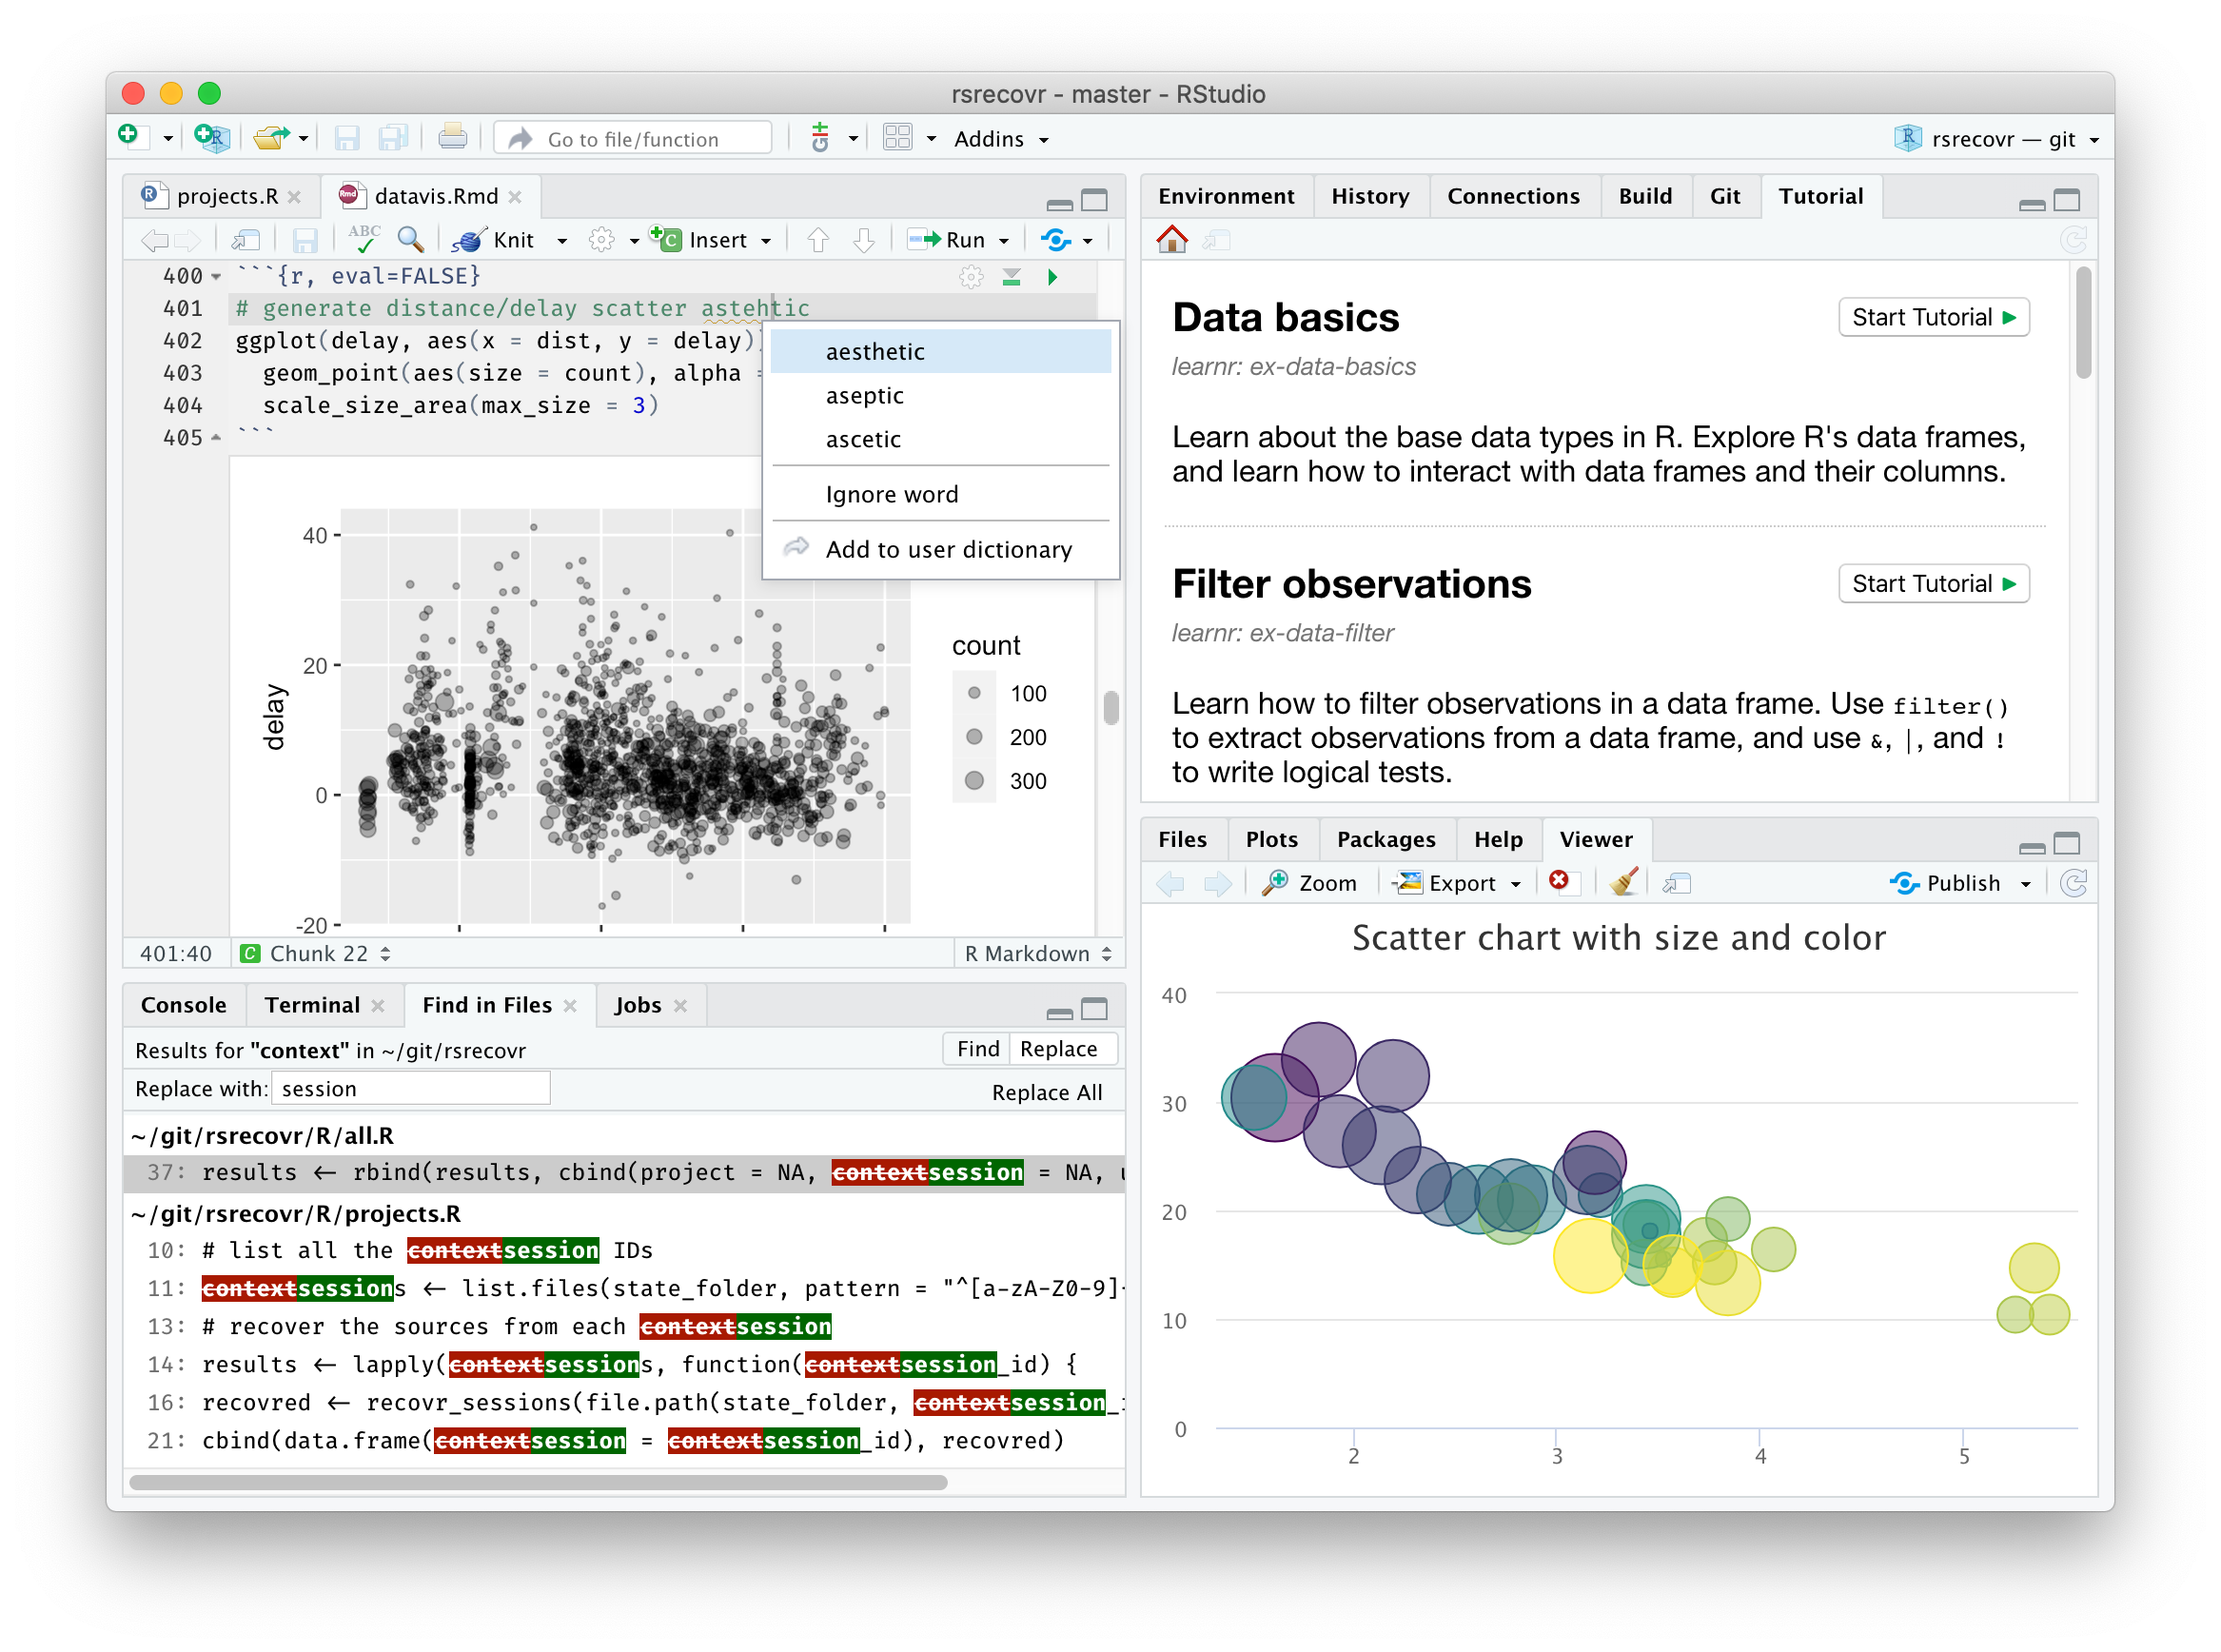
\includegraphics[keepaspectratio]{img/rstudio.png}}

}

\caption{Entorno de desarrollo RStudio}

\end{figure}%

\begin{itemize}
\tightlist
\item
  \href{https://rkward.kde.org}{RKWard}. Es otra otro de los entornos de
  desarrollo más completos que además incluye a posibilidad de añadir
  nuevos menús y cuadros de diálogo personalizados.
\end{itemize}

\begin{figure}[H]

{\centering \pandocbounded{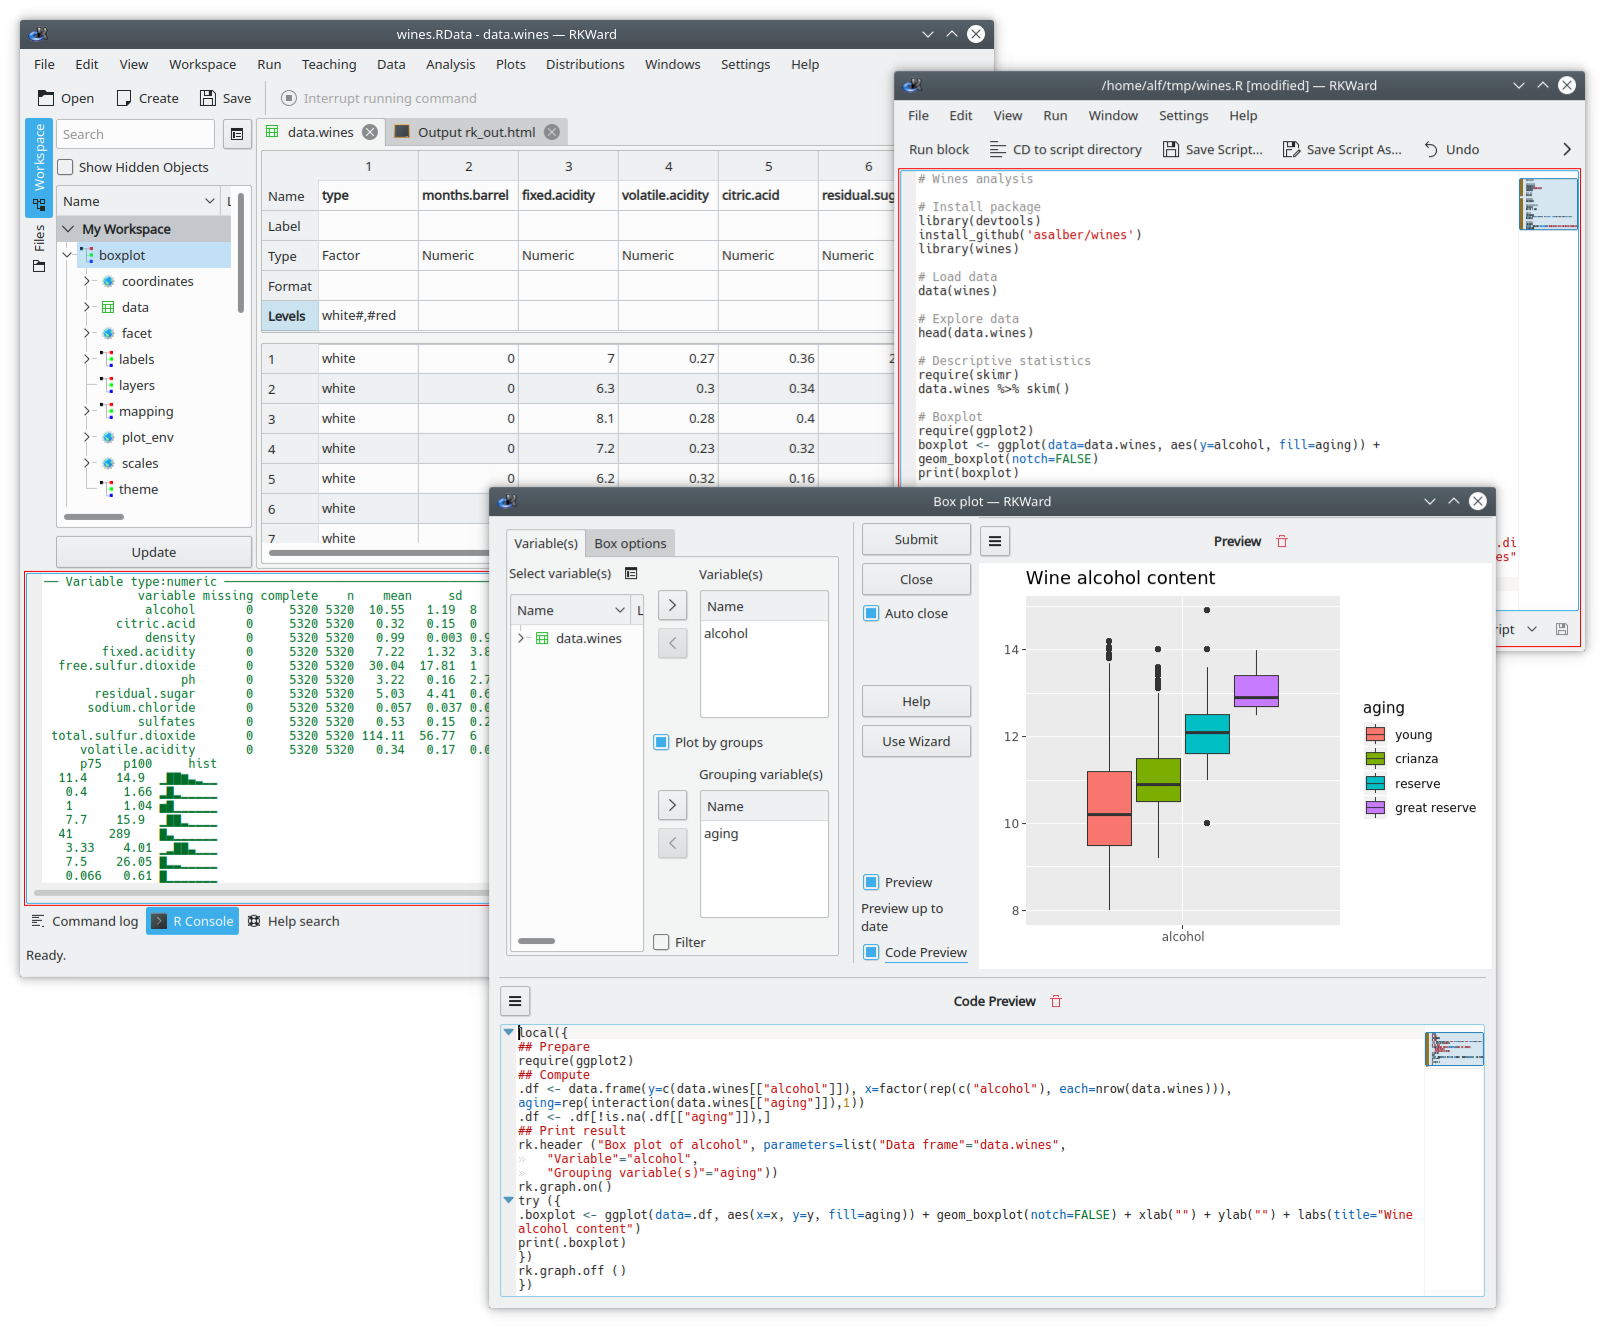
\includegraphics[keepaspectratio]{img/rkward.png}}

}

\caption{Entorno de desarrollo RKWard}

\end{figure}%

\begin{itemize}
\tightlist
\item
  \href{https://jupyter.org/}{Jupyter Lab}. Es un entorno de desarrollo
  interactivo que permite la creación de documentos que contienen
  código, texto, gráficos. Aunque no es un entorno de desarrollo
  específico para R, incluye un kernel para R que permite ejecutar
  código R en los documentos.
\end{itemize}

\begin{figure}[H]

{\centering \pandocbounded{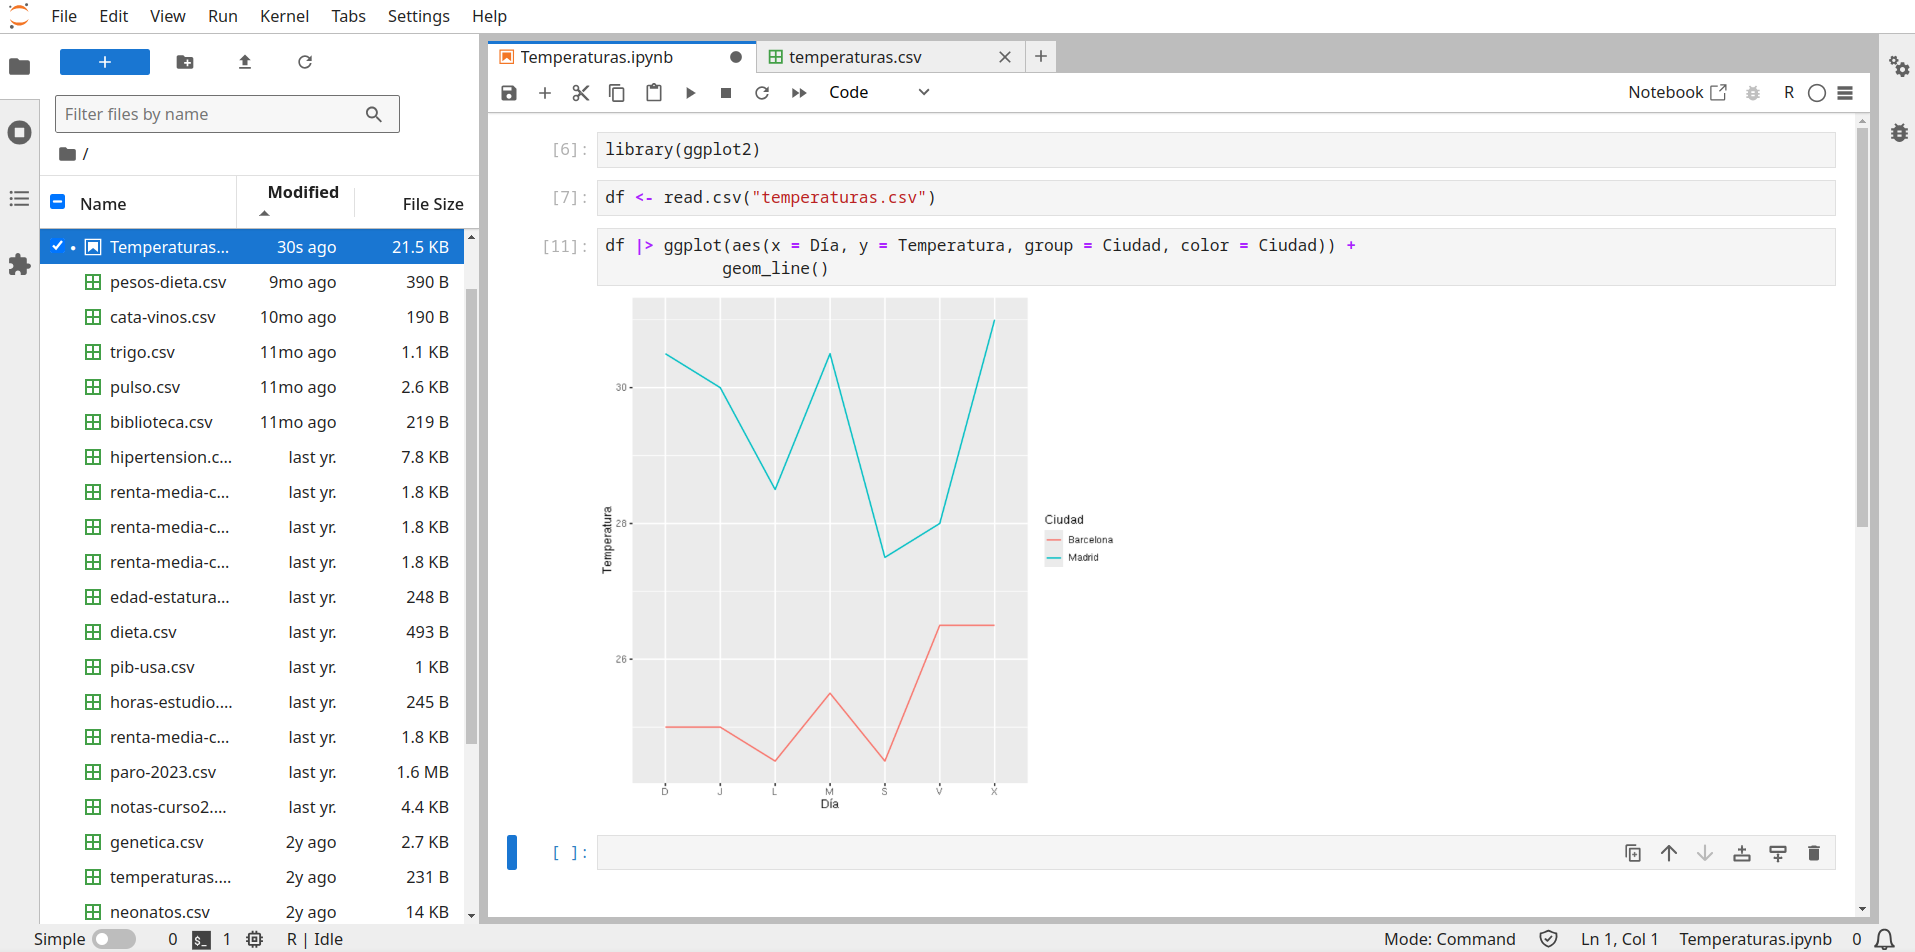
\includegraphics[keepaspectratio]{img/jupyter-lab.png}}

}

\caption{Entorno de desarrollo Jupyter Lab}

\end{figure}%

\begin{itemize}
\tightlist
\item
  \href{https://code.visualstudio.com/}{Visual Studio Code}. Es un
  entorno de desarrollo de propósito general ampliamente extendido.
  Aunque no es un entorno de desarrollo específico para R, incluye una
  extensión con utilidades que facilitan mucho el desarrollo con R.
\end{itemize}

\begin{figure}[H]

{\centering \pandocbounded{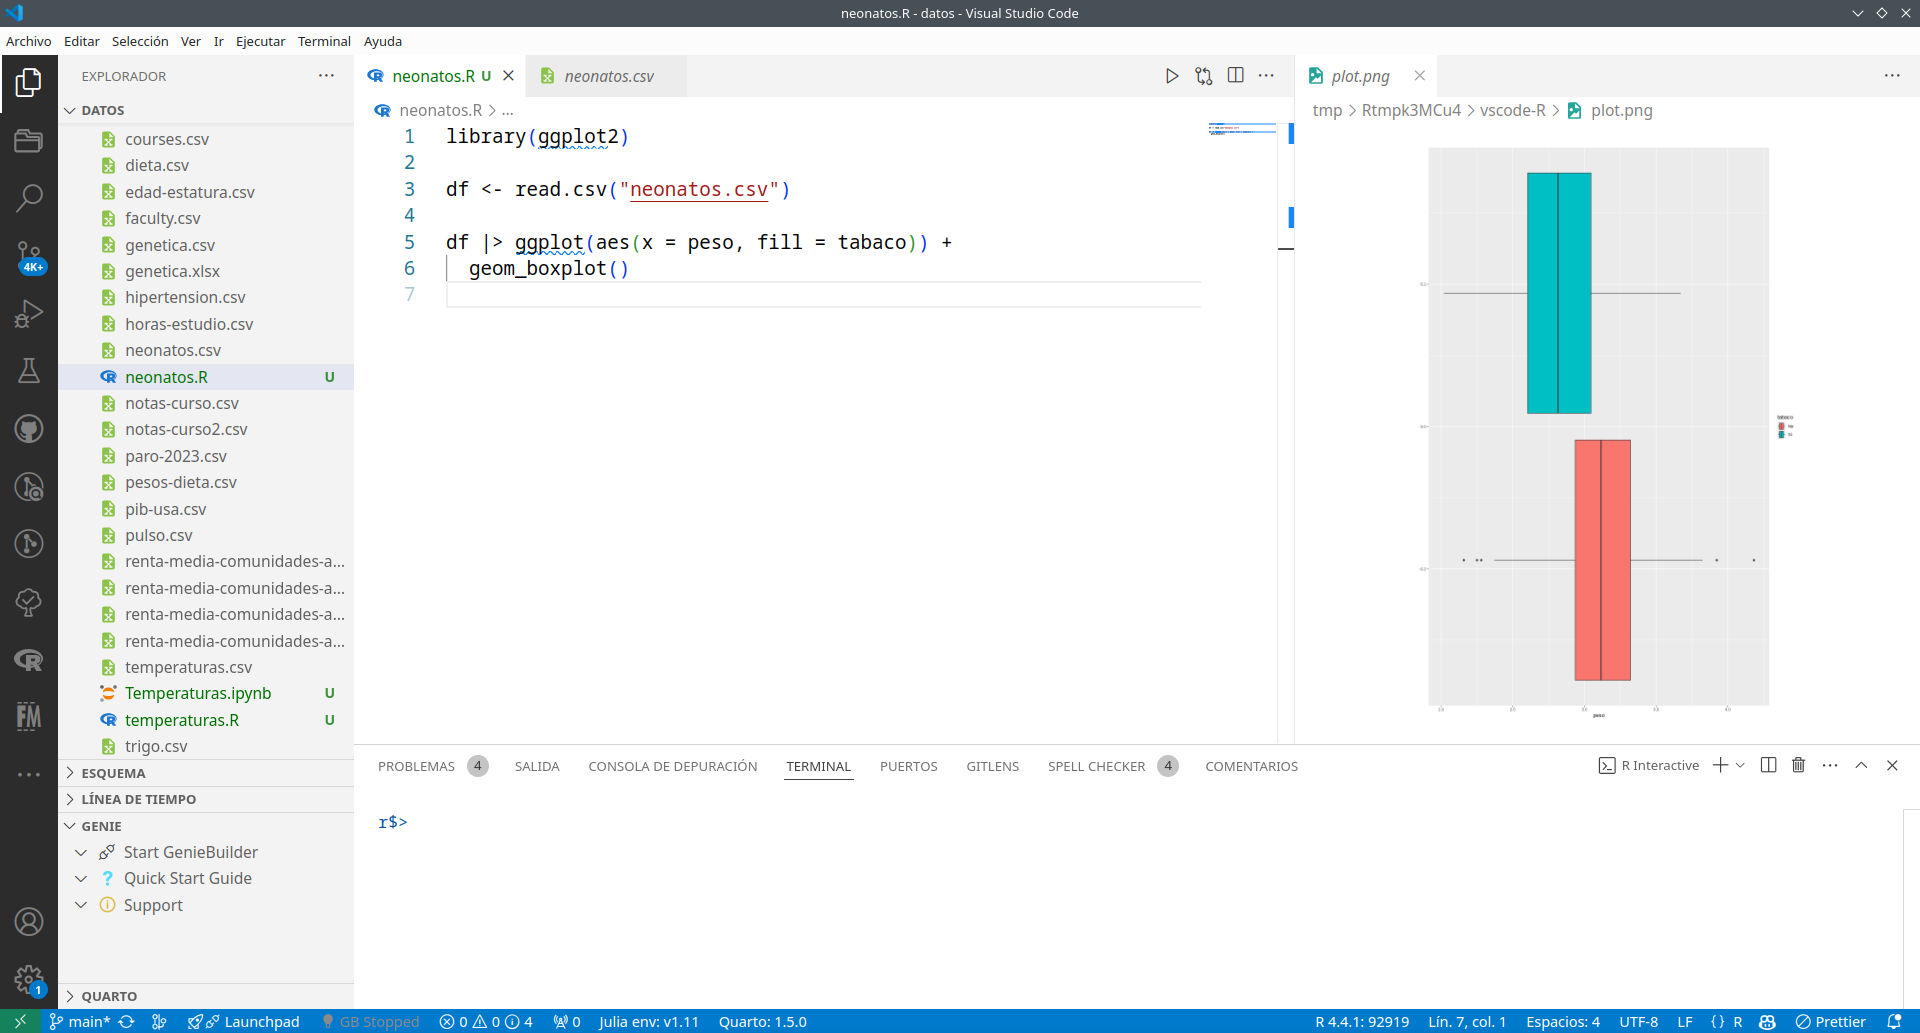
\includegraphics[keepaspectratio]{img/vscode-r.png}}

}

\caption{Entorno de desarrollo Visual Studio Code}

\end{figure}%

\section{Instalación de paquetes}\label{instalaciuxf3n-de-paquetes}

R es un lenguaje de programación modular, lo que significa que su
funcionalidad se extiende mediante paquetes. Los paquetes son
colecciones de funciones, datos y documentación sobre el uso de esas
funciones o conjuntos de datos.

El repositorio de paquetes más importante es
\href{https://cran.r-project.org/}{CRAN} (Comprehensive R Archive
Network), pero existen otros repositorios como
\href{https://www.bioconductor.org/}{Bioconductor} que contiene paquetes
específicos para el análisis de datos biológicos.

\subsection{Instalación de paquetes desde
CRAN}\label{instalaciuxf3n-de-paquetes-desde-cran}

Para instalar un paquete en R basta con ejecutar la función
\texttt{install.packages()} con el nombre del paquete que se desea
instalar. Por ejemplo, para instalar el paquete \texttt{ggplot2} que es
uno de los paquetes más utilizados para realizar gráficos en R, basta
con ejecutar el siguiente comando:

\begin{Shaded}
\begin{Highlighting}[]
\FunctionTok{install.packages}\NormalTok{(}\StringTok{"ggplot2"}\NormalTok{)}
\end{Highlighting}
\end{Shaded}

Los ubicación de los paquete instalados en R depende del sistema
operativo, pero puede consultarse en la variable \texttt{.libPaths()}.

\subsection{Instalación de paquetes desde
Bioconductor}\label{instalaciuxf3n-de-paquetes-desde-bioconductor}

Para instalar un paquete desde Bioconductor es necesario instalar
primero el paquete \texttt{BiocManager} y después utilizar la función
\texttt{BiocManager::install()} con el nombre del paquete que se desea
instalar. Por ejemplo, para instalar el paquete \texttt{DESeq2} que es
uno de los paquetes más utilizados para el análisis de datos de
expresión génica, basta con ejecutar el siguiente comando:

\begin{Shaded}
\begin{Highlighting}[]
\FunctionTok{install.packages}\NormalTok{(}\StringTok{"BiocManager"}\NormalTok{)}
\NormalTok{BiocManager}\SpecialCharTok{::}\FunctionTok{install}\NormalTok{(}\StringTok{"DESeq2"}\NormalTok{)}
\end{Highlighting}
\end{Shaded}

\section{Actualización de paquetes}\label{actualizaciuxf3n-de-paquetes}

Cada cierto tiempo conviene actualizar los paquetes instalados en R para
asegurarse de que se dispone de las últimas versiones de los mismos.
Para ello se puede utilizar la función \texttt{update.packages()}. Por
ejemplo, para actualizar todos los paquetes instalados en R sin
necesidad de confirmación por parte del usuario, basta con ejecutar el
siguiente comando:

\begin{Shaded}
\begin{Highlighting}[]
\FunctionTok{update.packages}\NormalTok{(}\AttributeTok{ask =} \ConstantTok{FALSE}\NormalTok{)}
\end{Highlighting}
\end{Shaded}

\bookmarksetup{startatroot}

\chapter{Tipos y estructuras de
datos}\label{tipos-y-estructuras-de-datos}

Esta práctica contiene ejercicios que muestran cómo trabajar con los
tipos y estructuras de datos en R. En concreto, las estructuras de datos
que se utilizan son

\begin{itemize}
\tightlist
\item
  Vectores.
\item
  Factores.
\item
  Matrices.
\item
  Listas.
\item
  Dataframes.
\end{itemize}

\section{Ejercicios Resueltos}\label{ejercicios-resueltos}

Para la realización de esta práctica se requieren los siguientes
paquetes.

\begin{Shaded}
\begin{Highlighting}[]
\FunctionTok{library}\NormalTok{(tidyverse) }
\CommentTok{\# Incluye los siguientes paquetes:}
\CommentTok{\# {-} readr: para la lectura de ficheros csv. }
\CommentTok{\# {-} dplyr: para el preprocesamiento y manipulación de datos.}
\FunctionTok{library}\NormalTok{(knitr) }\CommentTok{\# Para el formateo de tablas.}
\end{Highlighting}
\end{Shaded}

\begin{exercise}[]\protect\hypertarget{exr-vectores-1}{}\label{exr-vectores-1}

Realizar las siguientes operaciones con vectores.

\begin{enumerate}
\def\labelenumi{\alph{enumi}.}
\item
  Crear un vector con los números del 1 al 10.

  \begin{tcolorbox}[enhanced jigsaw, breakable, leftrule=.75mm, toptitle=1mm, rightrule=.15mm, opacitybacktitle=0.6, left=2mm, colframe=quarto-callout-tip-color-frame, titlerule=0mm, toprule=.15mm, opacityback=0, bottomtitle=1mm, coltitle=black, colbacktitle=quarto-callout-tip-color!10!white, title=\textcolor{quarto-callout-tip-color}{\faLightbulb}\hspace{0.5em}{Solución}, arc=.35mm, bottomrule=.15mm, colback=white]

  \section{Función c}

  La función \texttt{c()} permite combinar elementos en un vector. Los
  elementos se introducen separados por comas.

\begin{Shaded}
\begin{Highlighting}[]
\NormalTok{numeros }\OtherTok{\textless{}{-}} \FunctionTok{c}\NormalTok{(}\DecValTok{1}\NormalTok{, }\DecValTok{2}\NormalTok{, }\DecValTok{3}\NormalTok{, }\DecValTok{4}\NormalTok{, }\DecValTok{5}\NormalTok{, }\DecValTok{6}\NormalTok{, }\DecValTok{7}\NormalTok{, }\DecValTok{8}\NormalTok{, }\DecValTok{9}\NormalTok{, }\DecValTok{10}\NormalTok{)}
\NormalTok{numeros}
\end{Highlighting}
\end{Shaded}

\begin{verbatim}
 [1]  1  2  3  4  5  6  7  8  9 10
\end{verbatim}

  \section{Operador :}

  El operador \texttt{inicio:fin} permite crear un vector con la
  secuencia de números enteros desde el número \texttt{inicio} hasta el
  número \texttt{fin}.

\begin{Shaded}
\begin{Highlighting}[]
\NormalTok{numeros }\OtherTok{\textless{}{-}} \DecValTok{1}\SpecialCharTok{:}\DecValTok{10}
\NormalTok{numeros}
\end{Highlighting}
\end{Shaded}

\begin{verbatim}
 [1]  1  2  3  4  5  6  7  8  9 10
\end{verbatim}

  \end{tcolorbox}
\item
  Mostrar el número de elementos del vector anterior.

  \begin{tcolorbox}[enhanced jigsaw, breakable, leftrule=.75mm, toptitle=1mm, rightrule=.15mm, opacitybacktitle=0.6, left=2mm, colframe=quarto-callout-tip-color-frame, titlerule=0mm, toprule=.15mm, opacityback=0, bottomtitle=1mm, coltitle=black, colbacktitle=quarto-callout-tip-color!10!white, title=\textcolor{quarto-callout-tip-color}{\faLightbulb}\hspace{0.5em}{Solución}, arc=.35mm, bottomrule=.15mm, colback=white]

\begin{Shaded}
\begin{Highlighting}[]
\FunctionTok{length}\NormalTok{(numeros)}
\end{Highlighting}
\end{Shaded}

\begin{verbatim}
[1] 10
\end{verbatim}

  \end{tcolorbox}
\item
  Crear un vector con los números pares del 1 al 10.

  \begin{tcolorbox}[enhanced jigsaw, breakable, leftrule=.75mm, toptitle=1mm, rightrule=.15mm, opacitybacktitle=0.6, left=2mm, colframe=quarto-callout-tip-color-frame, titlerule=0mm, toprule=.15mm, opacityback=0, bottomtitle=1mm, coltitle=black, colbacktitle=quarto-callout-tip-color!10!white, title=\textcolor{quarto-callout-tip-color}{\faLightbulb}\hspace{0.5em}{Solución}, arc=.35mm, bottomrule=.15mm, colback=white]

  \section{Función c}

\begin{Shaded}
\begin{Highlighting}[]
\NormalTok{pares }\OtherTok{\textless{}{-}} \FunctionTok{c}\NormalTok{(}\DecValTok{2}\NormalTok{, }\DecValTok{4}\NormalTok{, }\DecValTok{6}\NormalTok{, }\DecValTok{8}\NormalTok{, }\DecValTok{10}\NormalTok{)}
\NormalTok{pares}
\end{Highlighting}
\end{Shaded}

\begin{verbatim}
[1]  2  4  6  8 10
\end{verbatim}

  \section{Función seq}

  La función \texttt{seq(inicio,\ fin,\ salto)} permite crear un vector
  con la secuencia de números enteros desde el número \texttt{inicio}
  hasta el número \texttt{fin} con un salto de \texttt{salto}.

\begin{Shaded}
\begin{Highlighting}[]
\NormalTok{pares }\OtherTok{\textless{}{-}} \FunctionTok{seq}\NormalTok{(}\DecValTok{2}\NormalTok{, }\DecValTok{10}\NormalTok{, }\AttributeTok{by =} \DecValTok{2}\NormalTok{)}
\NormalTok{pares}
\end{Highlighting}
\end{Shaded}

\begin{verbatim}
[1]  2  4  6  8 10
\end{verbatim}

  \end{tcolorbox}
\item
  Crear un vector con el cuadrado de los elementos del vector anterior.

  \begin{tcolorbox}[enhanced jigsaw, breakable, leftrule=.75mm, toptitle=1mm, rightrule=.15mm, opacitybacktitle=0.6, left=2mm, colframe=quarto-callout-tip-color-frame, titlerule=0mm, toprule=.15mm, opacityback=0, bottomtitle=1mm, coltitle=black, colbacktitle=quarto-callout-tip-color!10!white, title=\textcolor{quarto-callout-tip-color}{\faLightbulb}\hspace{0.5em}{Solución}, arc=.35mm, bottomrule=.15mm, colback=white]

  El operador \texttt{\^{}} permite elevar un número a otro. Cuando se
  aplica a un vector, eleva cada elemento del vector al número indicado.

\begin{Shaded}
\begin{Highlighting}[]
\NormalTok{cuadrados }\OtherTok{\textless{}{-}}\NormalTok{ pares}\SpecialCharTok{\^{}}\DecValTok{2}
\NormalTok{cuadrados}
\end{Highlighting}
\end{Shaded}

\begin{verbatim}
[1]   4  16  36  64 100
\end{verbatim}

  \end{tcolorbox}
\item
  Crear un vector con 5 números aleatorios entre 1 y 10.

  \begin{tcolorbox}[enhanced jigsaw, breakable, leftrule=.75mm, toptitle=1mm, rightrule=.15mm, opacitybacktitle=0.6, left=2mm, colframe=quarto-callout-tip-color-frame, titlerule=0mm, toprule=.15mm, opacityback=0, bottomtitle=1mm, coltitle=black, colbacktitle=quarto-callout-tip-color!10!white, title=\textcolor{quarto-callout-tip-color}{\faLightbulb}\hspace{0.5em}{Solución}, arc=.35mm, bottomrule=.15mm, colback=white]

  La función \texttt{sample(vector,\ n)} permite seleccionar \texttt{n}
  elementos aleatorios de \texttt{vector}. El muestreo es sin
  reemplazamiento.

\begin{Shaded}
\begin{Highlighting}[]
\NormalTok{aleatorios }\OtherTok{\textless{}{-}} \FunctionTok{sample}\NormalTok{(}\DecValTok{1}\SpecialCharTok{:}\DecValTok{10}\NormalTok{, }\DecValTok{5}\NormalTok{)}
\NormalTok{aleatorios}
\end{Highlighting}
\end{Shaded}

\begin{verbatim}
[1] 6 3 8 4 7
\end{verbatim}

  \end{tcolorbox}
\item
  Crear un vector booleano con los números del vector anterior que son
  pares.

  \begin{tcolorbox}[enhanced jigsaw, breakable, leftrule=.75mm, toptitle=1mm, rightrule=.15mm, opacitybacktitle=0.6, left=2mm, colframe=quarto-callout-tip-color-frame, titlerule=0mm, toprule=.15mm, opacityback=0, bottomtitle=1mm, coltitle=black, colbacktitle=quarto-callout-tip-color!10!white, title=\textcolor{quarto-callout-tip-color}{\faLightbulb}\hspace{0.5em}{Solución}, arc=.35mm, bottomrule=.15mm, colback=white]

  El operador \texttt{\%\%} permite calcular el resto de la división
  entera de dos números. Si el resto es 0, el número es par. Y el
  operador \texttt{==} permite comparar dos vectores elemento a
  elemento.

\begin{Shaded}
\begin{Highlighting}[]
\NormalTok{par }\OtherTok{\textless{}{-}}\NormalTok{ aleatorios }\SpecialCharTok{\%\%} \DecValTok{2} \SpecialCharTok{==} \DecValTok{0}
\NormalTok{par}
\end{Highlighting}
\end{Shaded}

\begin{verbatim}
[1]  TRUE FALSE  TRUE  TRUE FALSE
\end{verbatim}

  \end{tcolorbox}
\item
  Crear un vector con 100 números aleatorios entre 0 y 1.

  \begin{tcolorbox}[enhanced jigsaw, breakable, leftrule=.75mm, toptitle=1mm, rightrule=.15mm, opacitybacktitle=0.6, left=2mm, colframe=quarto-callout-tip-color-frame, titlerule=0mm, toprule=.15mm, opacityback=0, bottomtitle=1mm, coltitle=black, colbacktitle=quarto-callout-tip-color!10!white, title=\textcolor{quarto-callout-tip-color}{\faLightbulb}\hspace{0.5em}{Solución}, arc=.35mm, bottomrule=.15mm, colback=white]

  La función \texttt{runif(n,\ min,\ max)} permite generar \texttt{n}
  números aleatorios entre \texttt{min} y \texttt{max}.

\begin{Shaded}
\begin{Highlighting}[]
\NormalTok{aleatorios2 }\OtherTok{\textless{}{-}} \FunctionTok{runif}\NormalTok{(}\DecValTok{100}\NormalTok{, }\DecValTok{0}\NormalTok{, }\DecValTok{1}\NormalTok{)}
\NormalTok{aleatorios2}
\end{Highlighting}
\end{Shaded}

\begin{verbatim}
  [1] 0.1745409642 0.8289490622 0.3387814090 0.2167543538 0.1134076703
  [6] 0.6286752101 0.0106526525 0.1093907864 0.4900617937 0.1743749664
 [11] 0.6800843242 0.3646354883 0.6454122416 0.6526214175 0.9228122986
 [16] 0.3606315583 0.9950923640 0.3035428333 0.3958196980 0.2882284960
 [21] 0.2466872018 0.7218768313 0.6346673232 0.1410502058 0.8611289370
 [26] 0.0003058636 0.3754426709 0.4195440877 0.8103933139 0.9372969284
 [31] 0.7834821693 0.5671130815 0.3657950263 0.5821609648 0.1728922669
 [36] 0.1561128458 0.5271299311 0.3742025893 0.0244430660 0.1007965880
 [41] 0.3624238258 0.5429654324 0.7071530661 0.8355117675 0.5359205685
 [46] 0.3299977432 0.8245965624 0.3711511579 0.3284018056 0.7122194655
 [51] 0.7498793411 0.0470338808 0.0745800762 0.0610937241 0.8508216981
 [56] 0.9843574974 0.5178964895 0.8918249931 0.3667059876 0.1444752673
 [61] 0.3411170160 0.7664597644 0.4821867910 0.1529245593 0.7845511439
 [66] 0.3426257242 0.2204916265 0.6151761415 0.7651914931 0.2320692504
 [71] 0.4251030553 0.0818873062 0.2786484116 0.3453063101 0.4440597491
 [76] 0.0636016356 0.8731953043 0.7871375214 0.6084885013 0.6492142531
 [81] 0.6086444778 0.0130130642 0.2902684920 0.3225914293 0.1915048878
 [86] 0.8669210437 0.3068271666 0.7916705245 0.4637930305 0.8580898261
 [91] 0.8771222837 0.3976583821 0.5987865699 0.8512456813 0.5968641667
 [96] 0.1862874334 0.9470176871 0.8725937384 0.8956902823 0.4447817269
\end{verbatim}

  \end{tcolorbox}
\item
  Ordenar el vector anterior de menor a mayor.

  \begin{tcolorbox}[enhanced jigsaw, breakable, leftrule=.75mm, toptitle=1mm, rightrule=.15mm, opacitybacktitle=0.6, left=2mm, colframe=quarto-callout-tip-color-frame, titlerule=0mm, toprule=.15mm, opacityback=0, bottomtitle=1mm, coltitle=black, colbacktitle=quarto-callout-tip-color!10!white, title=\textcolor{quarto-callout-tip-color}{\faLightbulb}\hspace{0.5em}{Solución}, arc=.35mm, bottomrule=.15mm, colback=white]

  La función \texttt{sort(vector)} permite ordenar los elementos de un
  vector de menor a mayor.

\begin{Shaded}
\begin{Highlighting}[]
\FunctionTok{sort}\NormalTok{(aleatorios2)}
\end{Highlighting}
\end{Shaded}

\begin{verbatim}
  [1] 0.0003058636 0.0106526525 0.0130130642 0.0244430660 0.0470338808
  [6] 0.0610937241 0.0636016356 0.0745800762 0.0818873062 0.1007965880
 [11] 0.1093907864 0.1134076703 0.1410502058 0.1444752673 0.1529245593
 [16] 0.1561128458 0.1728922669 0.1743749664 0.1745409642 0.1862874334
 [21] 0.1915048878 0.2167543538 0.2204916265 0.2320692504 0.2466872018
 [26] 0.2786484116 0.2882284960 0.2902684920 0.3035428333 0.3068271666
 [31] 0.3225914293 0.3284018056 0.3299977432 0.3387814090 0.3411170160
 [36] 0.3426257242 0.3453063101 0.3606315583 0.3624238258 0.3646354883
 [41] 0.3657950263 0.3667059876 0.3711511579 0.3742025893 0.3754426709
 [46] 0.3958196980 0.3976583821 0.4195440877 0.4251030553 0.4440597491
 [51] 0.4447817269 0.4637930305 0.4821867910 0.4900617937 0.5178964895
 [56] 0.5271299311 0.5359205685 0.5429654324 0.5671130815 0.5821609648
 [61] 0.5968641667 0.5987865699 0.6084885013 0.6086444778 0.6151761415
 [66] 0.6286752101 0.6346673232 0.6454122416 0.6492142531 0.6526214175
 [71] 0.6800843242 0.7071530661 0.7122194655 0.7218768313 0.7498793411
 [76] 0.7651914931 0.7664597644 0.7834821693 0.7845511439 0.7871375214
 [81] 0.7916705245 0.8103933139 0.8245965624 0.8289490622 0.8355117675
 [86] 0.8508216981 0.8512456813 0.8580898261 0.8611289370 0.8669210437
 [91] 0.8725937384 0.8731953043 0.8771222837 0.8918249931 0.8956902823
 [96] 0.9228122986 0.9372969284 0.9470176871 0.9843574974 0.9950923640
\end{verbatim}

  \end{tcolorbox}
\item
  Ordenar el vector anterior de mayor a menor.

  \begin{tcolorbox}[enhanced jigsaw, breakable, leftrule=.75mm, toptitle=1mm, rightrule=.15mm, opacitybacktitle=0.6, left=2mm, colframe=quarto-callout-tip-color-frame, titlerule=0mm, toprule=.15mm, opacityback=0, bottomtitle=1mm, coltitle=black, colbacktitle=quarto-callout-tip-color!10!white, title=\textcolor{quarto-callout-tip-color}{\faLightbulb}\hspace{0.5em}{Solución}, arc=.35mm, bottomrule=.15mm, colback=white]

  La función \texttt{sort(vector,\ decreasing\ =\ TRUE)} permite ordenar
  los elementos de un vector de mayor a menor.

\begin{Shaded}
\begin{Highlighting}[]
\FunctionTok{sort}\NormalTok{(aleatorios2, }\AttributeTok{decreasing =} \ConstantTok{TRUE}\NormalTok{)}
\end{Highlighting}
\end{Shaded}

\begin{verbatim}
  [1] 0.9950923640 0.9843574974 0.9470176871 0.9372969284 0.9228122986
  [6] 0.8956902823 0.8918249931 0.8771222837 0.8731953043 0.8725937384
 [11] 0.8669210437 0.8611289370 0.8580898261 0.8512456813 0.8508216981
 [16] 0.8355117675 0.8289490622 0.8245965624 0.8103933139 0.7916705245
 [21] 0.7871375214 0.7845511439 0.7834821693 0.7664597644 0.7651914931
 [26] 0.7498793411 0.7218768313 0.7122194655 0.7071530661 0.6800843242
 [31] 0.6526214175 0.6492142531 0.6454122416 0.6346673232 0.6286752101
 [36] 0.6151761415 0.6086444778 0.6084885013 0.5987865699 0.5968641667
 [41] 0.5821609648 0.5671130815 0.5429654324 0.5359205685 0.5271299311
 [46] 0.5178964895 0.4900617937 0.4821867910 0.4637930305 0.4447817269
 [51] 0.4440597491 0.4251030553 0.4195440877 0.3976583821 0.3958196980
 [56] 0.3754426709 0.3742025893 0.3711511579 0.3667059876 0.3657950263
 [61] 0.3646354883 0.3624238258 0.3606315583 0.3453063101 0.3426257242
 [66] 0.3411170160 0.3387814090 0.3299977432 0.3284018056 0.3225914293
 [71] 0.3068271666 0.3035428333 0.2902684920 0.2882284960 0.2786484116
 [76] 0.2466872018 0.2320692504 0.2204916265 0.2167543538 0.1915048878
 [81] 0.1862874334 0.1745409642 0.1743749664 0.1728922669 0.1561128458
 [86] 0.1529245593 0.1444752673 0.1410502058 0.1134076703 0.1093907864
 [91] 0.1007965880 0.0818873062 0.0745800762 0.0636016356 0.0610937241
 [96] 0.0470338808 0.0244430660 0.0130130642 0.0106526525 0.0003058636
\end{verbatim}

  \end{tcolorbox}
\item
  Crear un vector con los días laborables de la semana.

  \begin{tcolorbox}[enhanced jigsaw, breakable, leftrule=.75mm, toptitle=1mm, rightrule=.15mm, opacitybacktitle=0.6, left=2mm, colframe=quarto-callout-tip-color-frame, titlerule=0mm, toprule=.15mm, opacityback=0, bottomtitle=1mm, coltitle=black, colbacktitle=quarto-callout-tip-color!10!white, title=\textcolor{quarto-callout-tip-color}{\faLightbulb}\hspace{0.5em}{Solución}, arc=.35mm, bottomrule=.15mm, colback=white]

\begin{Shaded}
\begin{Highlighting}[]
\NormalTok{dias\_laborables }\OtherTok{\textless{}{-}} \FunctionTok{c}\NormalTok{(}\StringTok{"Lunes"}\NormalTok{, }\StringTok{"Martes"}\NormalTok{, }\StringTok{"Miércoles"}\NormalTok{, }\StringTok{"Jueves"}\NormalTok{, }\StringTok{"Viernes"}\NormalTok{)}
\NormalTok{dias\_laborables}
\end{Highlighting}
\end{Shaded}

\begin{verbatim}
[1] "Lunes"     "Martes"    "Miércoles" "Jueves"    "Viernes"  
\end{verbatim}

  \end{tcolorbox}
\item
  Añadir los días del fin de semana al vector anterior y guardar el
  resultado en una nueva variable.

  \begin{tcolorbox}[enhanced jigsaw, breakable, leftrule=.75mm, toptitle=1mm, rightrule=.15mm, opacitybacktitle=0.6, left=2mm, colframe=quarto-callout-tip-color-frame, titlerule=0mm, toprule=.15mm, opacityback=0, bottomtitle=1mm, coltitle=black, colbacktitle=quarto-callout-tip-color!10!white, title=\textcolor{quarto-callout-tip-color}{\faLightbulb}\hspace{0.5em}{Solución}, arc=.35mm, bottomrule=.15mm, colback=white]

\begin{Shaded}
\begin{Highlighting}[]
\NormalTok{dias }\OtherTok{\textless{}{-}} \FunctionTok{c}\NormalTok{(dias\_laborables, }\StringTok{"Sábado"}\NormalTok{, }\StringTok{"Domingo"}\NormalTok{)}
\NormalTok{dias}
\end{Highlighting}
\end{Shaded}

\begin{verbatim}
[1] "Lunes"     "Martes"    "Miércoles" "Jueves"    "Viernes"  
[6] "Sábado"    "Domingo"  
\end{verbatim}

  \end{tcolorbox}
\item
  Acceder al tercer elemento del vector.

  \begin{tcolorbox}[enhanced jigsaw, breakable, leftrule=.75mm, toptitle=1mm, rightrule=.15mm, opacitybacktitle=0.6, left=2mm, colframe=quarto-callout-tip-color-frame, titlerule=0mm, toprule=.15mm, opacityback=0, bottomtitle=1mm, coltitle=black, colbacktitle=quarto-callout-tip-color!10!white, title=\textcolor{quarto-callout-tip-color}{\faLightbulb}\hspace{0.5em}{Solución}, arc=.35mm, bottomrule=.15mm, colback=white]

\begin{Shaded}
\begin{Highlighting}[]
\NormalTok{dias\_laborables[}\DecValTok{3}\NormalTok{]}
\end{Highlighting}
\end{Shaded}

\begin{verbatim}
[1] "Miércoles"
\end{verbatim}

  \end{tcolorbox}
\item
  Seleccionar los días pares del vector.

  \begin{tcolorbox}[enhanced jigsaw, breakable, leftrule=.75mm, toptitle=1mm, rightrule=.15mm, opacitybacktitle=0.6, left=2mm, colframe=quarto-callout-tip-color-frame, titlerule=0mm, toprule=.15mm, opacityback=0, bottomtitle=1mm, coltitle=black, colbacktitle=quarto-callout-tip-color!10!white, title=\textcolor{quarto-callout-tip-color}{\faLightbulb}\hspace{0.5em}{Solución}, arc=.35mm, bottomrule=.15mm, colback=white]

  \section{Índices numéricos}

\begin{Shaded}
\begin{Highlighting}[]
\NormalTok{dias[}\FunctionTok{c}\NormalTok{(}\DecValTok{2}\NormalTok{, }\DecValTok{4}\NormalTok{, }\DecValTok{6}\NormalTok{)]}
\end{Highlighting}
\end{Shaded}

\begin{verbatim}
[1] "Martes" "Jueves" "Sábado"
\end{verbatim}

  \section{Índices numéricos negativos}

\begin{Shaded}
\begin{Highlighting}[]
\NormalTok{dias[}\SpecialCharTok{{-}}\FunctionTok{c}\NormalTok{(}\DecValTok{1}\NormalTok{, }\DecValTok{3}\NormalTok{, }\DecValTok{5}\NormalTok{, }\DecValTok{7}\NormalTok{)]}
\end{Highlighting}
\end{Shaded}

\begin{verbatim}
[1] "Martes" "Jueves" "Sábado"
\end{verbatim}

  \section{Índices lógicos}

\begin{Shaded}
\begin{Highlighting}[]
\NormalTok{dias[}\FunctionTok{c}\NormalTok{(}\ConstantTok{FALSE}\NormalTok{, }\ConstantTok{TRUE}\NormalTok{)]}
\end{Highlighting}
\end{Shaded}

\begin{verbatim}
[1] "Martes" "Jueves" "Sábado"
\end{verbatim}

  \end{tcolorbox}
\item
  Concatenar los elementos del vector en una cadena de texto.

  \begin{tcolorbox}[enhanced jigsaw, breakable, leftrule=.75mm, toptitle=1mm, rightrule=.15mm, opacitybacktitle=0.6, left=2mm, colframe=quarto-callout-tip-color-frame, titlerule=0mm, toprule=.15mm, opacityback=0, bottomtitle=1mm, coltitle=black, colbacktitle=quarto-callout-tip-color!10!white, title=\textcolor{quarto-callout-tip-color}{\faLightbulb}\hspace{0.5em}{Solución}, arc=.35mm, bottomrule=.15mm, colback=white]

  La función \texttt{paste(vector,\ collapse\ =\ "\ ")} permite
  concatenar los elementos de un vector en una cadena de texto separados
  por un espacio.

\begin{Shaded}
\begin{Highlighting}[]
\FunctionTok{paste}\NormalTok{(dias, }\AttributeTok{collapse =} \StringTok{" "}\NormalTok{)}
\end{Highlighting}
\end{Shaded}

\begin{verbatim}
[1] "Lunes Martes Miércoles Jueves Viernes Sábado Domingo"
\end{verbatim}

  \end{tcolorbox}
\item
  Concatenar los elementos del vector en una cadena de texto separados
  por comas.

  \begin{tcolorbox}[enhanced jigsaw, breakable, leftrule=.75mm, toptitle=1mm, rightrule=.15mm, opacitybacktitle=0.6, left=2mm, colframe=quarto-callout-tip-color-frame, titlerule=0mm, toprule=.15mm, opacityback=0, bottomtitle=1mm, coltitle=black, colbacktitle=quarto-callout-tip-color!10!white, title=\textcolor{quarto-callout-tip-color}{\faLightbulb}\hspace{0.5em}{Solución}, arc=.35mm, bottomrule=.15mm, colback=white]

\begin{Shaded}
\begin{Highlighting}[]
\NormalTok{semana }\OtherTok{\textless{}{-}} \FunctionTok{paste}\NormalTok{(dias, }\AttributeTok{collapse =} \StringTok{", "}\NormalTok{)}
\NormalTok{semana}
\end{Highlighting}
\end{Shaded}

\begin{verbatim}
[1] "Lunes, Martes, Miércoles, Jueves, Viernes, Sábado, Domingo"
\end{verbatim}

  \end{tcolorbox}
\item
  Dividir la cadena anterior en subcadenas usando como separador la
  coma.

  \begin{tcolorbox}[enhanced jigsaw, breakable, leftrule=.75mm, toptitle=1mm, rightrule=.15mm, opacitybacktitle=0.6, left=2mm, colframe=quarto-callout-tip-color-frame, titlerule=0mm, toprule=.15mm, opacityback=0, bottomtitle=1mm, coltitle=black, colbacktitle=quarto-callout-tip-color!10!white, title=\textcolor{quarto-callout-tip-color}{\faLightbulb}\hspace{0.5em}{Solución}, arc=.35mm, bottomrule=.15mm, colback=white]

  La función \texttt{strsplit(cadena,\ separador)} permite dividir una
  cadena de texto en subcadenas usando como separador el valor de
  \texttt{separador}.

\begin{Shaded}
\begin{Highlighting}[]
\FunctionTok{strsplit}\NormalTok{(semana, }\StringTok{", "}\NormalTok{)}
\end{Highlighting}
\end{Shaded}

\begin{verbatim}
[[1]]
[1] "Lunes"     "Martes"    "Miércoles" "Jueves"    "Viernes"  
[6] "Sábado"    "Domingo"  
\end{verbatim}

  \end{tcolorbox}
\end{enumerate}

\end{exercise}

\begin{exercise}[]\protect\hypertarget{exr-factores-1}{}\label{exr-factores-1}

Se ha tomado una muestra de alumnos de una clase y se ha recogido la
información sobre el sexo de los alumnos obteniendo los siguientes
datos:

\[
\mbox{Mujer, Hombre, Mujer, Hombre, Mujer, Mujer, Hombre, Hombre}
\]

\begin{enumerate}
\def\labelenumi{\alph{enumi}.}
\item
  Crear un vector con los datos de la muestra.

  \begin{tcolorbox}[enhanced jigsaw, breakable, leftrule=.75mm, toptitle=1mm, rightrule=.15mm, opacitybacktitle=0.6, left=2mm, colframe=quarto-callout-tip-color-frame, titlerule=0mm, toprule=.15mm, opacityback=0, bottomtitle=1mm, coltitle=black, colbacktitle=quarto-callout-tip-color!10!white, title=\textcolor{quarto-callout-tip-color}{\faLightbulb}\hspace{0.5em}{Solución}, arc=.35mm, bottomrule=.15mm, colback=white]

\begin{Shaded}
\begin{Highlighting}[]
\NormalTok{sexo }\OtherTok{\textless{}{-}} \FunctionTok{c}\NormalTok{(}\StringTok{"Mujer"}\NormalTok{, }\StringTok{"Hombre"}\NormalTok{, }\StringTok{"Mujer"}\NormalTok{, }\StringTok{"Hombre"}\NormalTok{, }\StringTok{"Mujer"}\NormalTok{, }\StringTok{"Mujer"}\NormalTok{, }\StringTok{"Hombre"}\NormalTok{, }\StringTok{"Hombre"}\NormalTok{)}
\NormalTok{sexo}
\end{Highlighting}
\end{Shaded}

\begin{verbatim}
[1] "Mujer"  "Hombre" "Mujer"  "Hombre" "Mujer"  "Mujer"  "Hombre"
[8] "Hombre"
\end{verbatim}

  \end{tcolorbox}
\item
  Convertir el vector anterior en un factor.

  \begin{tcolorbox}[enhanced jigsaw, breakable, leftrule=.75mm, toptitle=1mm, rightrule=.15mm, opacitybacktitle=0.6, left=2mm, colframe=quarto-callout-tip-color-frame, titlerule=0mm, toprule=.15mm, opacityback=0, bottomtitle=1mm, coltitle=black, colbacktitle=quarto-callout-tip-color!10!white, title=\textcolor{quarto-callout-tip-color}{\faLightbulb}\hspace{0.5em}{Solución}, arc=.35mm, bottomrule=.15mm, colback=white]

  La función \texttt{factor(vector,\ labels)} permite convertir
  \texttt{vector} en un factor con los niveles o categorías
  especificados en \texttt{labels}. Si no se indica \texttt{labels}, los
  niveles se toman de los elementos del vector y se ordenan
  alfabéticamente.

\begin{Shaded}
\begin{Highlighting}[]
\NormalTok{sexo }\OtherTok{\textless{}{-}} \FunctionTok{factor}\NormalTok{(sexo)}
\NormalTok{sexo}
\end{Highlighting}
\end{Shaded}

\begin{verbatim}
[1] Mujer  Hombre Mujer  Hombre Mujer  Mujer  Hombre Hombre
Levels: Hombre Mujer
\end{verbatim}

  \end{tcolorbox}
\item
  Mostrar los niveles del factor.

  \begin{tcolorbox}[enhanced jigsaw, breakable, leftrule=.75mm, toptitle=1mm, rightrule=.15mm, opacitybacktitle=0.6, left=2mm, colframe=quarto-callout-tip-color-frame, titlerule=0mm, toprule=.15mm, opacityback=0, bottomtitle=1mm, coltitle=black, colbacktitle=quarto-callout-tip-color!10!white, title=\textcolor{quarto-callout-tip-color}{\faLightbulb}\hspace{0.5em}{Solución}, arc=.35mm, bottomrule=.15mm, colback=white]

  La función \texttt{levels(factor)} permite mostrar los niveles del
  factor \texttt{factor}.

\begin{Shaded}
\begin{Highlighting}[]
\FunctionTok{levels}\NormalTok{(sexo)}
\end{Highlighting}
\end{Shaded}

\begin{verbatim}
[1] "Hombre" "Mujer" 
\end{verbatim}

  \end{tcolorbox}
\item
  Reordenar los niveles del factor para que la categoría ``Mujer'' sea
  la primera.

  \begin{tcolorbox}[enhanced jigsaw, breakable, leftrule=.75mm, toptitle=1mm, rightrule=.15mm, opacitybacktitle=0.6, left=2mm, colframe=quarto-callout-tip-color-frame, titlerule=0mm, toprule=.15mm, opacityback=0, bottomtitle=1mm, coltitle=black, colbacktitle=quarto-callout-tip-color!10!white, title=\textcolor{quarto-callout-tip-color}{\faLightbulb}\hspace{0.5em}{Solución}, arc=.35mm, bottomrule=.15mm, colback=white]

\begin{Shaded}
\begin{Highlighting}[]
\NormalTok{sexo }\OtherTok{\textless{}{-}} \FunctionTok{factor}\NormalTok{(sexo, }\AttributeTok{levels =} \FunctionTok{c}\NormalTok{(}\StringTok{"Mujer"}\NormalTok{, }\StringTok{"Hombre"}\NormalTok{))}
\NormalTok{sexo}
\end{Highlighting}
\end{Shaded}

\begin{verbatim}
[1] Mujer  Hombre Mujer  Hombre Mujer  Mujer  Hombre Hombre
Levels: Mujer Hombre
\end{verbatim}

  \end{tcolorbox}
\end{enumerate}

\end{exercise}

\begin{exercise}[]\protect\hypertarget{exr-matrices-1}{}\label{exr-matrices-1}

Realizar las siguientes operaciones con matrices.

\begin{enumerate}
\def\labelenumi{\alph{enumi}.}
\item
  Crear una matriz de 2 filas y 2 columnas con los números del 1 al 4.

  \begin{tcolorbox}[enhanced jigsaw, breakable, leftrule=.75mm, toptitle=1mm, rightrule=.15mm, opacitybacktitle=0.6, left=2mm, colframe=quarto-callout-tip-color-frame, titlerule=0mm, toprule=.15mm, opacityback=0, bottomtitle=1mm, coltitle=black, colbacktitle=quarto-callout-tip-color!10!white, title=\textcolor{quarto-callout-tip-color}{\faLightbulb}\hspace{0.5em}{Solución}, arc=.35mm, bottomrule=.15mm, colback=white]

  La función \texttt{matrix(vector,\ nrow,\ ncol)} permite crear una
  matriz con los datos de \texttt{vector} el número de filas indicado en
  \texttt{nrow} y el número de columnas indicado en \texttt{ncol}.

\begin{Shaded}
\begin{Highlighting}[]
\NormalTok{A }\OtherTok{\textless{}{-}} \FunctionTok{matrix}\NormalTok{(}\DecValTok{1}\SpecialCharTok{:}\DecValTok{4}\NormalTok{, }\AttributeTok{nrow =} \DecValTok{2}\NormalTok{, }\AttributeTok{ncol =} \DecValTok{2}\NormalTok{)}
\NormalTok{A}
\end{Highlighting}
\end{Shaded}

\begin{verbatim}
     [,1] [,2]
[1,]    1    3
[2,]    2    4
\end{verbatim}

  \end{tcolorbox}
\item
  Añadir a la matriz anterior una nueva columna con los números del 5 y
  6.

  \begin{tcolorbox}[enhanced jigsaw, breakable, leftrule=.75mm, toptitle=1mm, rightrule=.15mm, opacitybacktitle=0.6, left=2mm, colframe=quarto-callout-tip-color-frame, titlerule=0mm, toprule=.15mm, opacityback=0, bottomtitle=1mm, coltitle=black, colbacktitle=quarto-callout-tip-color!10!white, title=\textcolor{quarto-callout-tip-color}{\faLightbulb}\hspace{0.5em}{Solución}, arc=.35mm, bottomrule=.15mm, colback=white]

  La función \texttt{cbind(matriz,\ vector)} permite añadir una nueva
  columna a la matriz \texttt{matriz} con los datos de \texttt{vector}.

\begin{Shaded}
\begin{Highlighting}[]
\NormalTok{A }\OtherTok{\textless{}{-}} \FunctionTok{cbind}\NormalTok{(A, }\DecValTok{5}\SpecialCharTok{:}\DecValTok{6}\NormalTok{)}
\NormalTok{A}
\end{Highlighting}
\end{Shaded}

\begin{verbatim}
     [,1] [,2] [,3]
[1,]    1    3    5
[2,]    2    4    6
\end{verbatim}

  \end{tcolorbox}
\item
  Crear una matriz de 2 filas y 2 columnas con los números del 1 al 4,
  rellenando los elementos por filas.

  \begin{tcolorbox}[enhanced jigsaw, breakable, leftrule=.75mm, toptitle=1mm, rightrule=.15mm, opacitybacktitle=0.6, left=2mm, colframe=quarto-callout-tip-color-frame, titlerule=0mm, toprule=.15mm, opacityback=0, bottomtitle=1mm, coltitle=black, colbacktitle=quarto-callout-tip-color!10!white, title=\textcolor{quarto-callout-tip-color}{\faLightbulb}\hspace{0.5em}{Solución}, arc=.35mm, bottomrule=.15mm, colback=white]

  La función \texttt{matrix} rellena los elementos de la matriz por
  columnas. Para rellenar los elementos por filas, se puede utilizar el
  parámetro opcional \texttt{byrow\ =\ TRUE}.

\begin{Shaded}
\begin{Highlighting}[]
\NormalTok{B }\OtherTok{\textless{}{-}} \FunctionTok{matrix}\NormalTok{(}\DecValTok{1}\SpecialCharTok{:}\DecValTok{4}\NormalTok{, }\AttributeTok{nrow =} \DecValTok{2}\NormalTok{, }\AttributeTok{ncol =} \DecValTok{2}\NormalTok{, }\AttributeTok{byrow =} \ConstantTok{TRUE}\NormalTok{)}
\NormalTok{B}
\end{Highlighting}
\end{Shaded}

\begin{verbatim}
     [,1] [,2]
[1,]    1    2
[2,]    3    4
\end{verbatim}

  \end{tcolorbox}
\item
  Crear otra matriz a partir de la anterior añadiendo una fila con los
  números 5 y 6.

  \begin{tcolorbox}[enhanced jigsaw, breakable, leftrule=.75mm, toptitle=1mm, rightrule=.15mm, opacitybacktitle=0.6, left=2mm, colframe=quarto-callout-tip-color-frame, titlerule=0mm, toprule=.15mm, opacityback=0, bottomtitle=1mm, coltitle=black, colbacktitle=quarto-callout-tip-color!10!white, title=\textcolor{quarto-callout-tip-color}{\faLightbulb}\hspace{0.5em}{Solución}, arc=.35mm, bottomrule=.15mm, colback=white]

\begin{Shaded}
\begin{Highlighting}[]
\NormalTok{B }\OtherTok{\textless{}{-}} \FunctionTok{rbind}\NormalTok{(B, }\DecValTok{5}\SpecialCharTok{:}\DecValTok{6}\NormalTok{)}
\NormalTok{B}
\end{Highlighting}
\end{Shaded}

\begin{verbatim}
     [,1] [,2]
[1,]    1    2
[2,]    3    4
[3,]    5    6
\end{verbatim}

  \end{tcolorbox}
\item
  Acceder al elemento de la segunda fila y la primera columna de la
  matriz anterior.

  \begin{tcolorbox}[enhanced jigsaw, breakable, leftrule=.75mm, toptitle=1mm, rightrule=.15mm, opacitybacktitle=0.6, left=2mm, colframe=quarto-callout-tip-color-frame, titlerule=0mm, toprule=.15mm, opacityback=0, bottomtitle=1mm, coltitle=black, colbacktitle=quarto-callout-tip-color!10!white, title=\textcolor{quarto-callout-tip-color}{\faLightbulb}\hspace{0.5em}{Solución}, arc=.35mm, bottomrule=.15mm, colback=white]

\begin{Shaded}
\begin{Highlighting}[]
\NormalTok{B[}\DecValTok{2}\NormalTok{, }\DecValTok{1}\NormalTok{]}
\end{Highlighting}
\end{Shaded}

\begin{verbatim}
[1] 3
\end{verbatim}

  \end{tcolorbox}
\item
  Seleccionar la primera fila de la matriz.

  \begin{tcolorbox}[enhanced jigsaw, breakable, leftrule=.75mm, toptitle=1mm, rightrule=.15mm, opacitybacktitle=0.6, left=2mm, colframe=quarto-callout-tip-color-frame, titlerule=0mm, toprule=.15mm, opacityback=0, bottomtitle=1mm, coltitle=black, colbacktitle=quarto-callout-tip-color!10!white, title=\textcolor{quarto-callout-tip-color}{\faLightbulb}\hspace{0.5em}{Solución}, arc=.35mm, bottomrule=.15mm, colback=white]

\begin{Shaded}
\begin{Highlighting}[]
\NormalTok{B[}\DecValTok{1}\NormalTok{, ]}
\end{Highlighting}
\end{Shaded}

\begin{verbatim}
[1] 1 2
\end{verbatim}

  \end{tcolorbox}
\item
  Seleccionar la segunda columna de la matriz.

  \begin{tcolorbox}[enhanced jigsaw, breakable, leftrule=.75mm, toptitle=1mm, rightrule=.15mm, opacitybacktitle=0.6, left=2mm, colframe=quarto-callout-tip-color-frame, titlerule=0mm, toprule=.15mm, opacityback=0, bottomtitle=1mm, coltitle=black, colbacktitle=quarto-callout-tip-color!10!white, title=\textcolor{quarto-callout-tip-color}{\faLightbulb}\hspace{0.5em}{Solución}, arc=.35mm, bottomrule=.15mm, colback=white]

\begin{Shaded}
\begin{Highlighting}[]
\NormalTok{B[, }\DecValTok{2}\NormalTok{]}
\end{Highlighting}
\end{Shaded}

\begin{verbatim}
[1] 2 4 6
\end{verbatim}

  \end{tcolorbox}
\item
  Multiplicar la matriz A por la matriz B.

  \begin{tcolorbox}[enhanced jigsaw, breakable, leftrule=.75mm, toptitle=1mm, rightrule=.15mm, opacitybacktitle=0.6, left=2mm, colframe=quarto-callout-tip-color-frame, titlerule=0mm, toprule=.15mm, opacityback=0, bottomtitle=1mm, coltitle=black, colbacktitle=quarto-callout-tip-color!10!white, title=\textcolor{quarto-callout-tip-color}{\faLightbulb}\hspace{0.5em}{Solución}, arc=.35mm, bottomrule=.15mm, colback=white]

  La multiplicación de matrices se realiza con el operador
  \texttt{\%*\%}.

\begin{Shaded}
\begin{Highlighting}[]
\NormalTok{A }\SpecialCharTok{\%*\%}\NormalTok{ B}
\end{Highlighting}
\end{Shaded}

\begin{verbatim}
     [,1] [,2]
[1,]   35   44
[2,]   44   56
\end{verbatim}

  \end{tcolorbox}
\item
  Calcular la transpuesta de la matriz A.

  \begin{tcolorbox}[enhanced jigsaw, breakable, leftrule=.75mm, toptitle=1mm, rightrule=.15mm, opacitybacktitle=0.6, left=2mm, colframe=quarto-callout-tip-color-frame, titlerule=0mm, toprule=.15mm, opacityback=0, bottomtitle=1mm, coltitle=black, colbacktitle=quarto-callout-tip-color!10!white, title=\textcolor{quarto-callout-tip-color}{\faLightbulb}\hspace{0.5em}{Solución}, arc=.35mm, bottomrule=.15mm, colback=white]

  La función \texttt{t(matriz)} permite calcular la transpuesta de
  \texttt{matriz}.

\begin{Shaded}
\begin{Highlighting}[]
\FunctionTok{t}\NormalTok{(A)}
\end{Highlighting}
\end{Shaded}

\begin{verbatim}
     [,1] [,2]
[1,]    1    2
[2,]    3    4
[3,]    5    6
\end{verbatim}

  \end{tcolorbox}
\end{enumerate}

\end{exercise}

\begin{exercise}[]\protect\hypertarget{exr-listas-1}{}\label{exr-listas-1}

Realizar las siguientes operaciones con listas.

\begin{enumerate}
\def\labelenumi{\alph{enumi}.}
\item
  Crear una lista con los siguientes con los datos del siguiente alumno:

  \begin{itemize}
  \tightlist
  \item
    Nombre: Juan.
  \item
    Edad: 20 años.
  \end{itemize}

  \begin{tcolorbox}[enhanced jigsaw, breakable, leftrule=.75mm, toptitle=1mm, rightrule=.15mm, opacitybacktitle=0.6, left=2mm, colframe=quarto-callout-tip-color-frame, titlerule=0mm, toprule=.15mm, opacityback=0, bottomtitle=1mm, coltitle=black, colbacktitle=quarto-callout-tip-color!10!white, title=\textcolor{quarto-callout-tip-color}{\faLightbulb}\hspace{0.5em}{Solución}, arc=.35mm, bottomrule=.15mm, colback=white]

  Para crear una lista se utiliza la función
  \texttt{list(nombre1\ =\ valor1,\ nombre2\ =\ valor2,\ ...)}.

\begin{Shaded}
\begin{Highlighting}[]
\NormalTok{alumno }\OtherTok{\textless{}{-}} \FunctionTok{list}\NormalTok{(}\AttributeTok{Nombre =} \StringTok{"Juan"}\NormalTok{, }\AttributeTok{Edad =} \DecValTok{20}\NormalTok{)}
\NormalTok{alumno}
\end{Highlighting}
\end{Shaded}

\begin{verbatim}
$Nombre
[1] "Juan"

$Edad
[1] 20
\end{verbatim}

  \end{tcolorbox}
\item
  Obtener la edad del alumno.

  \begin{tcolorbox}[enhanced jigsaw, breakable, leftrule=.75mm, toptitle=1mm, rightrule=.15mm, opacitybacktitle=0.6, left=2mm, colframe=quarto-callout-tip-color-frame, titlerule=0mm, toprule=.15mm, opacityback=0, bottomtitle=1mm, coltitle=black, colbacktitle=quarto-callout-tip-color!10!white, title=\textcolor{quarto-callout-tip-color}{\faLightbulb}\hspace{0.5em}{Solución}, arc=.35mm, bottomrule=.15mm, colback=white]

  Para acceder a los elementos de una lista se utiliza el operador
  \texttt{\$}.

\begin{Shaded}
\begin{Highlighting}[]
\NormalTok{alumno}\SpecialCharTok{$}\NormalTok{Edad}
\end{Highlighting}
\end{Shaded}

\begin{verbatim}
[1] 20
\end{verbatim}

  \end{tcolorbox}
\item
  Crear una lista con las siguientes notas del alumno:

  \begin{itemize}
  \tightlist
  \item
    Matemáticas: 7.
  \item
    Química: 8.
  \end{itemize}

  \begin{tcolorbox}[enhanced jigsaw, breakable, leftrule=.75mm, toptitle=1mm, rightrule=.15mm, opacitybacktitle=0.6, left=2mm, colframe=quarto-callout-tip-color-frame, titlerule=0mm, toprule=.15mm, opacityback=0, bottomtitle=1mm, coltitle=black, colbacktitle=quarto-callout-tip-color!10!white, title=\textcolor{quarto-callout-tip-color}{\faLightbulb}\hspace{0.5em}{Solución}, arc=.35mm, bottomrule=.15mm, colback=white]

\begin{Shaded}
\begin{Highlighting}[]
\NormalTok{notas }\OtherTok{\textless{}{-}} \FunctionTok{list}\NormalTok{(Matemáticas }\OtherTok{=} \DecValTok{7}\NormalTok{, Química }\OtherTok{=} \DecValTok{8}\NormalTok{)}
\NormalTok{notas}
\end{Highlighting}
\end{Shaded}

\begin{verbatim}
$Matemáticas
[1] 7

$Química
[1] 8
\end{verbatim}

  \end{tcolorbox}
\item
  Añadir la lista de notas a la lista del alumno.

  \begin{tcolorbox}[enhanced jigsaw, breakable, leftrule=.75mm, toptitle=1mm, rightrule=.15mm, opacitybacktitle=0.6, left=2mm, colframe=quarto-callout-tip-color-frame, titlerule=0mm, toprule=.15mm, opacityback=0, bottomtitle=1mm, coltitle=black, colbacktitle=quarto-callout-tip-color!10!white, title=\textcolor{quarto-callout-tip-color}{\faLightbulb}\hspace{0.5em}{Solución}, arc=.35mm, bottomrule=.15mm, colback=white]

\begin{Shaded}
\begin{Highlighting}[]
\NormalTok{alumno}\SpecialCharTok{$}\NormalTok{Notas }\OtherTok{\textless{}{-}}\NormalTok{ notas}
\NormalTok{alumno}
\end{Highlighting}
\end{Shaded}

\begin{verbatim}
$Nombre
[1] "Juan"

$Edad
[1] 20

$Notas
$Notas$Matemáticas
[1] 7

$Notas$Química
[1] 8
\end{verbatim}

  \end{tcolorbox}
\item
  Añadir a la lista anterior la nota del examen de Física, que ha sido
  un 6.

  \begin{tcolorbox}[enhanced jigsaw, breakable, leftrule=.75mm, toptitle=1mm, rightrule=.15mm, opacitybacktitle=0.6, left=2mm, colframe=quarto-callout-tip-color-frame, titlerule=0mm, toprule=.15mm, opacityback=0, bottomtitle=1mm, coltitle=black, colbacktitle=quarto-callout-tip-color!10!white, title=\textcolor{quarto-callout-tip-color}{\faLightbulb}\hspace{0.5em}{Solución}, arc=.35mm, bottomrule=.15mm, colback=white]

\begin{Shaded}
\begin{Highlighting}[]
\NormalTok{alumno}\SpecialCharTok{$}\NormalTok{Notas}\SpecialCharTok{$}\NormalTok{Física }\OtherTok{\textless{}{-}} \DecValTok{6}
\NormalTok{alumno}
\end{Highlighting}
\end{Shaded}

\begin{verbatim}
$Nombre
[1] "Juan"

$Edad
[1] 20

$Notas
$Notas$Matemáticas
[1] 7

$Notas$Química
[1] 8

$Notas$Física
[1] 6
\end{verbatim}

  \end{tcolorbox}
\end{enumerate}

\end{exercise}

\begin{exercise}[]\protect\hypertarget{exr-dataframes-1}{}\label{exr-dataframes-1}

La siguiente tabla contiene los ingresos y gastos de una empresa durante
el primer trimestre del año.

\begin{longtable}[]{@{}lrrr@{}}
\toprule\noalign{}
Mes & Ingresos & Gastos & Impuestos \\
\midrule\noalign{}
\endhead
\bottomrule\noalign{}
\endlastfoot
Enero & 45000 & 33400 & 6450 \\
Febrero & 41500 & 35400 & 6300 \\
Marzo & 51200 & 35600 & 7100 \\
\end{longtable}

\begin{enumerate}
\def\labelenumi{\alph{enumi}.}
\item
  Crear un data frame con los datos de la tabla.

  \begin{tcolorbox}[enhanced jigsaw, breakable, leftrule=.75mm, toptitle=1mm, rightrule=.15mm, opacitybacktitle=0.6, left=2mm, colframe=quarto-callout-tip-color-frame, titlerule=0mm, toprule=.15mm, opacityback=0, bottomtitle=1mm, coltitle=black, colbacktitle=quarto-callout-tip-color!10!white, title=\textcolor{quarto-callout-tip-color}{\faLightbulb}\hspace{0.5em}{Solución}, arc=.35mm, bottomrule=.15mm, colback=white]

  Para crear un data frame se utiliza la función
  \texttt{data.frame(columna1\ =\ vector1,\ columna2\ =\ vector2,\ ...)},
  donde \texttt{columna1}, \texttt{columna2}, \ldots{} son los nombres
  de las columnas y \texttt{vector1}, \texttt{vector2}, \ldots{} son los
  vectores con los datos de cada columna, que deben tener la misma
  longitud.

\begin{Shaded}
\begin{Highlighting}[]
\NormalTok{df }\OtherTok{\textless{}{-}} \FunctionTok{data.frame}\NormalTok{(}
    \AttributeTok{Mes =} \FunctionTok{c}\NormalTok{(}\StringTok{"Enero"}\NormalTok{, }\StringTok{"Febrero"}\NormalTok{, }\StringTok{"Marzo"}\NormalTok{),}
    \AttributeTok{Ingresos =} \FunctionTok{c}\NormalTok{(}\DecValTok{45000}\NormalTok{, }\DecValTok{41500}\NormalTok{, }\DecValTok{51200}\NormalTok{),}
    \AttributeTok{Gastos =} \FunctionTok{c}\NormalTok{(}\DecValTok{33400}\NormalTok{, }\DecValTok{35400}\NormalTok{, }\DecValTok{35600}\NormalTok{)}
\NormalTok{    )}
\NormalTok{df }
\end{Highlighting}
\end{Shaded}

  \begin{longtable}[]{@{}lrr@{}}
  \toprule\noalign{}
  Mes & Ingresos & Gastos \\
  \midrule\noalign{}
  \endhead
  \bottomrule\noalign{}
  \endlastfoot
  Enero & 45000 & 33400 \\
  Febrero & 41500 & 35400 \\
  Marzo & 51200 & 35600 \\
  \end{longtable}

  \end{tcolorbox}
\item
  Añadir una nueva columna con los siguientes impuestos pagados.

  \begin{longtable}[]{@{}lr@{}}
  \toprule\noalign{}
  Mes & Impuestos \\
  \midrule\noalign{}
  \endhead
  \bottomrule\noalign{}
  \endlastfoot
  Enero & 6450 \\
  Febrero & 6300 \\
  Marzo & 7100 \\
  \end{longtable}

  \begin{tcolorbox}[enhanced jigsaw, breakable, leftrule=.75mm, toptitle=1mm, rightrule=.15mm, opacitybacktitle=0.6, left=2mm, colframe=quarto-callout-tip-color-frame, titlerule=0mm, toprule=.15mm, opacityback=0, bottomtitle=1mm, coltitle=black, colbacktitle=quarto-callout-tip-color!10!white, title=\textcolor{quarto-callout-tip-color}{\faLightbulb}\hspace{0.5em}{Solución}, arc=.35mm, bottomrule=.15mm, colback=white]

  \section{Base}

  Con las funciones del paquete \texttt{base} de R.

\begin{Shaded}
\begin{Highlighting}[]
\NormalTok{df}\SpecialCharTok{$}\NormalTok{Impuestos }\OtherTok{\textless{}{-}} \FunctionTok{c}\NormalTok{(}\DecValTok{6450}\NormalTok{, }\DecValTok{6300}\NormalTok{, }\DecValTok{7100}\NormalTok{)}
\NormalTok{df}
\end{Highlighting}
\end{Shaded}

  \begin{longtable}[]{@{}lrrr@{}}
  \toprule\noalign{}
  Mes & Ingresos & Gastos & Impuestos \\
  \midrule\noalign{}
  \endhead
  \bottomrule\noalign{}
  \endlastfoot
  Enero & 45000 & 33400 & 6450 \\
  Febrero & 41500 & 35400 & 6300 \\
  Marzo & 51200 & 35600 & 7100 \\
  \end{longtable}

  \section{tidyverse}

  Con las funciones del paquete \texttt{dplyr} de \texttt{tidyverse}.

\begin{Shaded}
\begin{Highlighting}[]
\NormalTok{df }\OtherTok{\textless{}{-}}\NormalTok{ df }\SpecialCharTok{|\textgreater{}} \FunctionTok{mutate}\NormalTok{(}\AttributeTok{Impuestos =} \FunctionTok{c}\NormalTok{(}\DecValTok{6450}\NormalTok{, }\DecValTok{6300}\NormalTok{, }\DecValTok{7100}\NormalTok{))}
\NormalTok{df}
\end{Highlighting}
\end{Shaded}

  \begin{longtable}[]{@{}lrrr@{}}
  \toprule\noalign{}
  Mes & Ingresos & Gastos & Impuestos \\
  \midrule\noalign{}
  \endhead
  \bottomrule\noalign{}
  \endlastfoot
  Enero & 45000 & 33400 & 6450 \\
  Febrero & 41500 & 35400 & 6300 \\
  Marzo & 51200 & 35600 & 7100 \\
  \end{longtable}

  \end{tcolorbox}
\item
  Añadir una nueva fila con los siguientes datos de Abril.

  \begin{longtable}[]{@{}lrrr@{}}
  \toprule\noalign{}
  Mes & Ingresos & Gastos & Impuestos \\
  \midrule\noalign{}
  \endhead
  \bottomrule\noalign{}
  \endlastfoot
  Abril & 49700 & 36300 & 6850 \\
  \end{longtable}

  \begin{tcolorbox}[enhanced jigsaw, breakable, leftrule=.75mm, toptitle=1mm, rightrule=.15mm, opacitybacktitle=0.6, left=2mm, colframe=quarto-callout-tip-color-frame, titlerule=0mm, toprule=.15mm, opacityback=0, bottomtitle=1mm, coltitle=black, colbacktitle=quarto-callout-tip-color!10!white, title=\textcolor{quarto-callout-tip-color}{\faLightbulb}\hspace{0.5em}{Solución}, arc=.35mm, bottomrule=.15mm, colback=white]

  \section{Base}

  Con las funciones del paquete \texttt{base} de R.

\begin{Shaded}
\begin{Highlighting}[]
\NormalTok{df }\OtherTok{\textless{}{-}} \FunctionTok{rbind}\NormalTok{(df, }\FunctionTok{list}\NormalTok{(}\AttributeTok{Mes =} \StringTok{"Abril"}\NormalTok{, }\AttributeTok{Ingresos =} \DecValTok{49700}\NormalTok{, }\AttributeTok{Gastos =} \DecValTok{36300}\NormalTok{, }\AttributeTok{Impuestos =} \DecValTok{6850}\NormalTok{))}
\NormalTok{df}
\end{Highlighting}
\end{Shaded}

  \begin{longtable}[]{@{}lrrr@{}}
  \toprule\noalign{}
  Mes & Ingresos & Gastos & Impuestos \\
  \midrule\noalign{}
  \endhead
  \bottomrule\noalign{}
  \endlastfoot
  Enero & 45000 & 33400 & 6450 \\
  Febrero & 41500 & 35400 & 6300 \\
  Marzo & 51200 & 35600 & 7100 \\
  Abril & 49700 & 36300 & 6850 \\
  \end{longtable}

  \section{tidyverse}

  Con las funciones del paquete \texttt{dplyr} de \texttt{tidyverse}.

\begin{Shaded}
\begin{Highlighting}[]
\NormalTok{df }\OtherTok{\textless{}{-}}\NormalTok{ df }\SpecialCharTok{|\textgreater{}} \FunctionTok{add\_row}\NormalTok{(}\AttributeTok{Mes =} \StringTok{"Abril"}\NormalTok{, }\AttributeTok{Ingresos =} \DecValTok{49700}\NormalTok{, }\AttributeTok{Gastos =} \DecValTok{36300}\NormalTok{, }\AttributeTok{Impuestos =} \DecValTok{6850}\NormalTok{)}
\NormalTok{df}
\end{Highlighting}
\end{Shaded}

  \begin{longtable}[]{@{}lrrr@{}}
  \toprule\noalign{}
  Mes & Ingresos & Gastos & Impuestos \\
  \midrule\noalign{}
  \endhead
  \bottomrule\noalign{}
  \endlastfoot
  Enero & 45000 & 33400 & 6450 \\
  Febrero & 41500 & 35400 & 6300 \\
  Marzo & 51200 & 35600 & 7100 \\
  Abril & 49700 & 36300 & 6850 \\
  \end{longtable}

  \end{tcolorbox}
\item
  Cambiar los ingresos de Marzo por 50400.

  \begin{tcolorbox}[enhanced jigsaw, breakable, leftrule=.75mm, toptitle=1mm, rightrule=.15mm, opacitybacktitle=0.6, left=2mm, colframe=quarto-callout-tip-color-frame, titlerule=0mm, toprule=.15mm, opacityback=0, bottomtitle=1mm, coltitle=black, colbacktitle=quarto-callout-tip-color!10!white, title=\textcolor{quarto-callout-tip-color}{\faLightbulb}\hspace{0.5em}{Solución}, arc=.35mm, bottomrule=.15mm, colback=white]

\begin{Shaded}
\begin{Highlighting}[]
\NormalTok{df[}\DecValTok{3}\NormalTok{, }\StringTok{"Ingresos"}\NormalTok{] }\OtherTok{\textless{}{-}} \DecValTok{50400}
\NormalTok{df}
\end{Highlighting}
\end{Shaded}

  \begin{longtable}[]{@{}lrrr@{}}
  \toprule\noalign{}
  Mes & Ingresos & Gastos & Impuestos \\
  \midrule\noalign{}
  \endhead
  \bottomrule\noalign{}
  \endlastfoot
  Enero & 45000 & 33400 & 6450 \\
  Febrero & 41500 & 35400 & 6300 \\
  Marzo & 50400 & 35600 & 7100 \\
  Abril & 49700 & 36300 & 6850 \\
  \end{longtable}

  \end{tcolorbox}
\item
  Guardar el data frame en un fichero csv.

  \begin{tcolorbox}[enhanced jigsaw, breakable, leftrule=.75mm, toptitle=1mm, rightrule=.15mm, opacitybacktitle=0.6, left=2mm, colframe=quarto-callout-tip-color-frame, titlerule=0mm, toprule=.15mm, opacityback=0, bottomtitle=1mm, coltitle=black, colbacktitle=quarto-callout-tip-color!10!white, title=\textcolor{quarto-callout-tip-color}{\faLightbulb}\hspace{0.5em}{Solución}, arc=.35mm, bottomrule=.15mm, colback=white]

  La función \texttt{write.csv(dataframe,\ "fichero.csv")} permite
  guardar el data frame \texttt{dataframe} en el fichero
  \texttt{fichero.csv}.

\begin{Shaded}
\begin{Highlighting}[]
\FunctionTok{write.csv}\NormalTok{(df, }\StringTok{"datos/ingresos\_gastos.csv"}\NormalTok{, }\AttributeTok{row.names =} \ConstantTok{FALSE}\NormalTok{)}
\end{Highlighting}
\end{Shaded}

  \end{tcolorbox}
\end{enumerate}

\end{exercise}

\begin{exercise}[]\protect\hypertarget{exr-dataframes-2}{}\label{exr-dataframes-2}

El fichero \href{datos/colesterol.csv}{\texttt{colesterol.csv}} contiene
información de una muestra de pacientes donde se han medido la edad, el
sexo, el peso, la altura y el nivel de colesterol, además de su nombre.

\begin{enumerate}
\def\labelenumi{\alph{enumi}.}
\item
  Crear un data frame con los datos de todos los pacientes del estudio a
  partir del fichero
  \href{datos/colesterol.csv}{\texttt{colesterol.csv}} y mostrar las
  primeras filas.

  \begin{tcolorbox}[enhanced jigsaw, breakable, leftrule=.75mm, toptitle=1mm, rightrule=.15mm, opacitybacktitle=0.6, left=2mm, colframe=quarto-callout-tip-color-frame, titlerule=0mm, toprule=.15mm, opacityback=0, bottomtitle=1mm, coltitle=black, colbacktitle=quarto-callout-tip-color!10!white, title=\textcolor{quarto-callout-tip-color}{\faLightbulb}\hspace{0.5em}{Solución}, arc=.35mm, bottomrule=.15mm, colback=white]

  \section{Base}

  Con las funciones del paquete \texttt{base} de R. La función
  \texttt{read.csv("fichero.csv")} permite leer un fichero csv y cargar
  los datos en un data frame. Y la función \texttt{head(dataframe)}
  permite mostrar las primeras filas del data frame \texttt{dataframe}.

\begin{Shaded}
\begin{Highlighting}[]
\NormalTok{df }\OtherTok{\textless{}{-}} \FunctionTok{read.csv}\NormalTok{(}\StringTok{"https://aprendeconalf.es/estadistica{-}practicas{-}r/datos/colesterol.csv"}\NormalTok{)}
\FunctionTok{head}\NormalTok{(df)}
\end{Highlighting}
\end{Shaded}

  \begin{longtable}[]{@{}lrlrrr@{}}
  \toprule\noalign{}
  nombre & edad & sexo & peso & altura & colesterol \\
  \midrule\noalign{}
  \endhead
  \bottomrule\noalign{}
  \endlastfoot
  José Luis Martínez Izquierdo & 18 & H & 85 & 1.79 & 182 \\
  Rosa Díaz Díaz & 32 & M & 65 & 1.73 & 232 \\
  Javier García Sánchez & 24 & H & NA & 1.81 & 191 \\
  Carmen López Pinzón & 35 & M & 65 & 1.70 & 200 \\
  Marisa López Collado & 46 & M & 51 & 1.58 & 148 \\
  Antonio Ruiz Cruz & 68 & H & 66 & 1.74 & 249 \\
  \end{longtable}

  \section{tidyverse}

  Con la función
  \href{https://readr.tidyverse.org/reference/read_delim.html}{\texttt{read\_csv}}
  del paquete del paquete
  \href{https://readr.tidyverse.org/index.html}{\texttt{readr}} de
  \texttt{tidyverse}.

\begin{Shaded}
\begin{Highlighting}[]
\NormalTok{df }\OtherTok{\textless{}{-}} \FunctionTok{read\_csv}\NormalTok{(}\StringTok{"https://aprendeconalf.es/estadistica{-}practicas{-}r/datos/colesterol.csv"}\NormalTok{)}
\FunctionTok{head}\NormalTok{(df)}
\end{Highlighting}
\end{Shaded}

  \begin{longtable}[]{@{}lrlrrr@{}}
  \toprule\noalign{}
  nombre & edad & sexo & peso & altura & colesterol \\
  \midrule\noalign{}
  \endhead
  \bottomrule\noalign{}
  \endlastfoot
  José Luis Martínez Izquierdo & 18 & H & 85 & 1.79 & 182 \\
  Rosa Díaz Díaz & 32 & M & 65 & 1.73 & 232 \\
  Javier García Sánchez & 24 & H & NA & 1.81 & 191 \\
  Carmen López Pinzón & 35 & M & 65 & 1.70 & 200 \\
  Marisa López Collado & 46 & M & 51 & 1.58 & 148 \\
  Antonio Ruiz Cruz & 68 & H & 66 & 1.74 & 249 \\
  \end{longtable}

  \end{tcolorbox}
\item
  Mostrar las variables del data frame.

  \begin{tcolorbox}[enhanced jigsaw, breakable, leftrule=.75mm, toptitle=1mm, rightrule=.15mm, opacitybacktitle=0.6, left=2mm, colframe=quarto-callout-tip-color-frame, titlerule=0mm, toprule=.15mm, opacityback=0, bottomtitle=1mm, coltitle=black, colbacktitle=quarto-callout-tip-color!10!white, title=\textcolor{quarto-callout-tip-color}{\faLightbulb}\hspace{0.5em}{Solución}, arc=.35mm, bottomrule=.15mm, colback=white]

  \section{Base}

  Con las funciones del paquete \texttt{base} de R.

\begin{Shaded}
\begin{Highlighting}[]
\FunctionTok{colnames}\NormalTok{(df)}
\end{Highlighting}
\end{Shaded}

\begin{verbatim}
[1] "nombre"     "edad"       "sexo"       "peso"       "altura"    
[6] "colesterol"
\end{verbatim}

  \section{tidyverse}

  Con la función
  \href{https://dplyr.tidyverse.org/reference/glimpse.html?q=read_csv\#undefined}{\texttt{glimpse}}
  del paquete
  \href{https://dplyr.tidyverse.org/index.html}{\texttt{dplyr}} de
  \texttt{tidyverse}. Esta función muestra las columnas del data frame
  en filas, de manera que permite ver todas las columnas de un data
  frame cuando este tiene muchas columnas.

\begin{Shaded}
\begin{Highlighting}[]
\FunctionTok{glimpse}\NormalTok{(df)}
\end{Highlighting}
\end{Shaded}

\begin{verbatim}
Rows: 14
Columns: 6
$ nombre     <chr> "José Luis Martínez Izquierdo", "Rosa Díaz Díaz",~
$ edad       <dbl> 18, 32, 24, 35, 46, 68, 51, 22, 35, 46, 53, 58, 2~
$ sexo       <chr> "H", "M", "H", "M", "M", "H", "H", "M", "H", "H",~
$ peso       <dbl> 85, 65, NA, 65, 51, 66, 62, 60, 90, 75, 55, 78, 1~
$ altura     <dbl> 1.79, 1.73, 1.81, 1.70, 1.58, 1.74, 1.72, 1.66, 1~
$ colesterol <dbl> 182, 232, 191, 200, 148, 249, 276, NA, 241, 280, ~
\end{verbatim}

  \end{tcolorbox}
\item
  Mostrar el número de filas del data frame, que corresponde al número
  de pacientes.

  \begin{tcolorbox}[enhanced jigsaw, breakable, leftrule=.75mm, toptitle=1mm, rightrule=.15mm, opacitybacktitle=0.6, left=2mm, colframe=quarto-callout-tip-color-frame, titlerule=0mm, toprule=.15mm, opacityback=0, bottomtitle=1mm, coltitle=black, colbacktitle=quarto-callout-tip-color!10!white, title=\textcolor{quarto-callout-tip-color}{\faLightbulb}\hspace{0.5em}{Solución}, arc=.35mm, bottomrule=.15mm, colback=white]

  La función \texttt{nrow(dataframe)} permite mostrar el número de filas
  del data frame \texttt{dataframe}.

\begin{Shaded}
\begin{Highlighting}[]
\FunctionTok{nrow}\NormalTok{(df)}
\end{Highlighting}
\end{Shaded}

\begin{verbatim}
[1] 14
\end{verbatim}

  \end{tcolorbox}
\item
  Mostrar 5 filas aleatorias del data frame.

  \begin{tcolorbox}[enhanced jigsaw, breakable, leftrule=.75mm, toptitle=1mm, rightrule=.15mm, opacitybacktitle=0.6, left=2mm, colframe=quarto-callout-tip-color-frame, titlerule=0mm, toprule=.15mm, opacityback=0, bottomtitle=1mm, coltitle=black, colbacktitle=quarto-callout-tip-color!10!white, title=\textcolor{quarto-callout-tip-color}{\faLightbulb}\hspace{0.5em}{Solución}, arc=.35mm, bottomrule=.15mm, colback=white]

  \section{Base}

  La función \texttt{sample(vector,\ n)} permite seleccionar \texttt{n}
  elementos aleatorios de \texttt{vector}. El muestreo es sin
  reemplazamiento.

\begin{Shaded}
\begin{Highlighting}[]
\NormalTok{df[}\FunctionTok{sample}\NormalTok{(}\FunctionTok{nrow}\NormalTok{(df), }\DecValTok{5}\NormalTok{), ]}
\end{Highlighting}
\end{Shaded}

  \begin{longtable}[]{@{}lrlrrr@{}}
  \toprule\noalign{}
  nombre & edad & sexo & peso & altura & colesterol \\
  \midrule\noalign{}
  \endhead
  \bottomrule\noalign{}
  \endlastfoot
  Miguel Angel Cuadrado Gutiérrez & 27 & H & 109 & 1.98 & 210 \\
  José María de la Guía Sanz & 58 & H & 78 & 1.87 & 198 \\
  Antonio Fernández Ocaña & 51 & H & 62 & 1.72 & 276 \\
  Macarena Álvarez Luna & 53 & M & 55 & 1.62 & 262 \\
  Carmen López Pinzón & 35 & M & 65 & 1.70 & 200 \\
  \end{longtable}

  \section{tidyverse}

  La función \texttt{sample\_n(dataframe,\ n)} del paquete
  \texttt{dplyr} de \texttt{tidyverse} permite seleccionar \texttt{n}
  filas aleatorias del data frame \texttt{dataframe}.

\begin{Shaded}
\begin{Highlighting}[]
\NormalTok{df }\SpecialCharTok{|\textgreater{}} \FunctionTok{sample\_n}\NormalTok{(}\DecValTok{5}\NormalTok{)}
\end{Highlighting}
\end{Shaded}

  \begin{longtable}[]{@{}lrlrrr@{}}
  \toprule\noalign{}
  nombre & edad & sexo & peso & altura & colesterol \\
  \midrule\noalign{}
  \endhead
  \bottomrule\noalign{}
  \endlastfoot
  Marisa López Collado & 46 & M & 51 & 1.58 & 148 \\
  Antonio Fernández Ocaña & 51 & H & 62 & 1.72 & 276 \\
  Antonio Ruiz Cruz & 68 & H & 66 & 1.74 & 249 \\
  Carmen López Pinzón & 35 & M & 65 & 1.70 & 200 \\
  Javier García Sánchez & 24 & H & NA & 1.81 & 191 \\
  \end{longtable}

  \end{tcolorbox}
\item
  Obtener los datos de colesterol de los pacientes.

  \begin{tcolorbox}[enhanced jigsaw, breakable, leftrule=.75mm, toptitle=1mm, rightrule=.15mm, opacitybacktitle=0.6, left=2mm, colframe=quarto-callout-tip-color-frame, titlerule=0mm, toprule=.15mm, opacityback=0, bottomtitle=1mm, coltitle=black, colbacktitle=quarto-callout-tip-color!10!white, title=\textcolor{quarto-callout-tip-color}{\faLightbulb}\hspace{0.5em}{Solución}, arc=.35mm, bottomrule=.15mm, colback=white]

  \section{Base}

  Con las funciones del paquete \texttt{base} de R.

\begin{Shaded}
\begin{Highlighting}[]
\NormalTok{df}\SpecialCharTok{$}\NormalTok{colesterol}
\end{Highlighting}
\end{Shaded}

\begin{verbatim}
 [1] 182 232 191 200 148 249 276  NA 241 280 262 198 210 194
\end{verbatim}

  \section{tidyverse}

  Con la función
  \href{https://dplyr.tidyverse.org/reference/select.html}{\texttt{select}}
  del paquete
  \href{https://dplyr.tidyverse.org/index.html}{\texttt{dplyr}} de
  \texttt{tidyverse}.

\begin{Shaded}
\begin{Highlighting}[]
\NormalTok{df }\SpecialCharTok{|\textgreater{}} \FunctionTok{select}\NormalTok{(colesterol)}
\end{Highlighting}
\end{Shaded}

  \begin{longtable}[]{@{}r@{}}
  \toprule\noalign{}
  colesterol \\
  \midrule\noalign{}
  \endhead
  \bottomrule\noalign{}
  \endlastfoot
  182 \\
  232 \\
  191 \\
  200 \\
  148 \\
  249 \\
  276 \\
  NA \\
  241 \\
  280 \\
  262 \\
  198 \\
  210 \\
  194 \\
  \end{longtable}

  \end{tcolorbox}
\item
  Obtener los datos del quinto paciente.

  \begin{tcolorbox}[enhanced jigsaw, breakable, leftrule=.75mm, toptitle=1mm, rightrule=.15mm, opacitybacktitle=0.6, left=2mm, colframe=quarto-callout-tip-color-frame, titlerule=0mm, toprule=.15mm, opacityback=0, bottomtitle=1mm, coltitle=black, colbacktitle=quarto-callout-tip-color!10!white, title=\textcolor{quarto-callout-tip-color}{\faLightbulb}\hspace{0.5em}{Solución}, arc=.35mm, bottomrule=.15mm, colback=white]

  \section{Base}

  Con las funciones del paquete \texttt{base} de R.

\begin{Shaded}
\begin{Highlighting}[]
\NormalTok{df[}\DecValTok{5}\NormalTok{, ]}
\end{Highlighting}
\end{Shaded}

  \begin{longtable}[]{@{}lrlrrr@{}}
  \toprule\noalign{}
  nombre & edad & sexo & peso & altura & colesterol \\
  \midrule\noalign{}
  \endhead
  \bottomrule\noalign{}
  \endlastfoot
  Marisa López Collado & 46 & M & 51 & 1.58 & 148 \\
  \end{longtable}

  \section{tidyverse}

  Con la función
  \href{https://dplyr.tidyverse.org/reference/slice.html}{\texttt{slice}}
  del paquete
  \href{https://dplyr.tidyverse.org/index.html}{\texttt{dplyr}} de
  \texttt{tidyverse}.

\begin{Shaded}
\begin{Highlighting}[]
\NormalTok{df }\SpecialCharTok{|\textgreater{}} \FunctionTok{slice}\NormalTok{(}\DecValTok{5}\NormalTok{)}
\end{Highlighting}
\end{Shaded}

  \begin{longtable}[]{@{}lrlrrr@{}}
  \toprule\noalign{}
  nombre & edad & sexo & peso & altura & colesterol \\
  \midrule\noalign{}
  \endhead
  \bottomrule\noalign{}
  \endlastfoot
  Marisa López Collado & 46 & M & 51 & 1.58 & 148 \\
  \end{longtable}

  \end{tcolorbox}
\end{enumerate}

\end{exercise}

\section{Ejercicios Propuestos}\label{ejercicios-propuestos}

\begin{exercise}[]\protect\hypertarget{exr-vectores-2}{}\label{exr-vectores-2}

La siguiente tabla contiene las notas de un grupo de alumnos en dos
asignaturas.

\begin{longtable}[]{@{}llrr@{}}
\toprule\noalign{}
Alumno & Grupo & Física & Química \\
\midrule\noalign{}
\endhead
\bottomrule\noalign{}
\endlastfoot
Juan & A & 7.0 & 6.7 \\
María & B & 3.5 & 5.0 \\
Pedro & B & 6.0 & 7.1 \\
Ana & A & 5.2 & 4.5 \\
Luis & A & 4.5 & NA \\
Sara & B & 9.0 & 9.2 \\
\end{longtable}

\begin{enumerate}
\def\labelenumi{\alph{enumi}.}
\item
  Crear un vector con los nombres de los alumnos.
\item
  Crear un factor el grupo.
\item
  Crear un vector con las notas de Física y otro con las notas de
  Química.
\item
  Crear un vector con la nota media de las dos asignaturas.
\item
  Crear un vector booleano con los alumnos que han aprobado el curso.
  Para aprobar el curso, la nota media de las dos asignaturas debe ser
  mayor o igual a 5.
\item
  Crear un vector con los nombres de los alumnos que han aprobado el
  curso.
\item
  Crear un data frame con los nombres de los alumnos, sus notas y su
  media reutilizando los vectores anteriores.
\item
  Guardar el data frame en un fichero csv.
\end{enumerate}

\end{exercise}

\bookmarksetup{startatroot}

\chapter{Preprocesamiento de datos}\label{preprocesamiento-de-datos}

Esta práctica contiene ejercicios que muestran como preprocesar un
conjunto de datos en R. El preprocesamiento de datos es una tarea
fundamental en el análisis de datos que consiste en la limpieza,
transformación y preparación de los datos para su análisis. El
preprocesamiento de datos incluye tareas como

\begin{itemize}
\tightlist
\item
  Limpieza de datos.
\item
  Imputación de valores perdidos.
\item
  Recodificación de variables.
\item
  Creación de nuevas variables.
\item
  Transformación de variables.
\item
  Selección de variables.
\item
  Fusión de datos.
\item
  Reestructuración del conjunto de datos.
\end{itemize}

\section{Ejercicios Resueltos}\label{ejercicios-resueltos-1}

Para la realización de esta práctica se requieren los siguientes
paquetes.

\begin{Shaded}
\begin{Highlighting}[]
\FunctionTok{library}\NormalTok{(tidyverse) }
\CommentTok{\# Incluye los siguientes paquetes:}
\CommentTok{\# {-} readr: para la lectura de ficheros csv. }
\CommentTok{\# {-} dplyr: para el preprocesamiento y manipulación de datos.}
\CommentTok{\# {-} lubridate: para el procesamiento de fechas.}
\FunctionTok{library}\NormalTok{(knitr) }\CommentTok{\# Para el formateo de tablas.}
\end{Highlighting}
\end{Shaded}

\begin{exercise}[]\protect\hypertarget{exr-preprocesamiento-1}{}\label{exr-preprocesamiento-1}

La siguiente tabla contiene los ingresos y gastos de una empresa durante
el primer trimestre del año.

\begin{longtable}[]{@{}lrrr@{}}
\toprule\noalign{}
Mes & Ingresos & Gastos & Impuestos \\
\midrule\noalign{}
\endhead
\bottomrule\noalign{}
\endlastfoot
Enero & 45000 & 33400 & 6450 \\
Febrero & 41500 & 35400 & 6300 \\
Marzo & 51200 & 35600 & 7100 \\
Abril & 49700 & 36300 & 6850 \\
\end{longtable}

\begin{enumerate}
\def\labelenumi{\alph{enumi}.}
\item
  Crear un data frame con los datos de la tabla.

  \begin{tcolorbox}[enhanced jigsaw, breakable, leftrule=.75mm, toptitle=1mm, rightrule=.15mm, opacitybacktitle=0.6, left=2mm, colframe=quarto-callout-tip-color-frame, titlerule=0mm, toprule=.15mm, opacityback=0, bottomtitle=1mm, coltitle=black, colbacktitle=quarto-callout-tip-color!10!white, title=\textcolor{quarto-callout-tip-color}{\faLightbulb}\hspace{0.5em}{Solución}, arc=.35mm, bottomrule=.15mm, colback=white]

\begin{Shaded}
\begin{Highlighting}[]
\NormalTok{df }\OtherTok{\textless{}{-}} \FunctionTok{data.frame}\NormalTok{(}
    \AttributeTok{Mes =} \FunctionTok{c}\NormalTok{(}\StringTok{"Enero"}\NormalTok{, }\StringTok{"Febrero"}\NormalTok{, }\StringTok{"Marzo"}\NormalTok{, }\StringTok{"Abril"}\NormalTok{),}
    \AttributeTok{Ingresos =} \FunctionTok{c}\NormalTok{(}\DecValTok{45000}\NormalTok{, }\DecValTok{41500}\NormalTok{, }\DecValTok{51200}\NormalTok{, }\DecValTok{49700}\NormalTok{),}
    \AttributeTok{Gastos =} \FunctionTok{c}\NormalTok{(}\DecValTok{33400}\NormalTok{, }\DecValTok{35400}\NormalTok{, }\DecValTok{35600}\NormalTok{, }\DecValTok{36300}\NormalTok{),}
    \AttributeTok{Impuestos =} \FunctionTok{c}\NormalTok{(}\DecValTok{6450}\NormalTok{, }\DecValTok{6300}\NormalTok{, }\DecValTok{7100}\NormalTok{, }\DecValTok{6850}\NormalTok{)}
\NormalTok{    )}
\NormalTok{df }
\end{Highlighting}
\end{Shaded}

\begin{verbatim}
      Mes Ingresos Gastos Impuestos
1   Enero    45000  33400      6450
2 Febrero    41500  35400      6300
3   Marzo    51200  35600      7100
4   Abril    49700  36300      6850
\end{verbatim}

  \end{tcolorbox}
\item
  Crear una nueva columna con los beneficios de cada mes (ingresos -
  gastos - impuestos).

  \begin{tcolorbox}[enhanced jigsaw, breakable, leftrule=.75mm, toptitle=1mm, rightrule=.15mm, opacitybacktitle=0.6, left=2mm, colframe=quarto-callout-tip-color-frame, titlerule=0mm, toprule=.15mm, opacityback=0, bottomtitle=1mm, coltitle=black, colbacktitle=quarto-callout-tip-color!10!white, title=\textcolor{quarto-callout-tip-color}{\faLightbulb}\hspace{0.5em}{Solución}, arc=.35mm, bottomrule=.15mm, colback=white]

  \section{Base}

  Con las funciones del paquete \texttt{base} de R.

\begin{Shaded}
\begin{Highlighting}[]
\NormalTok{df}\SpecialCharTok{$}\NormalTok{Beneficios }\OtherTok{\textless{}{-}}\NormalTok{ df}\SpecialCharTok{$}\NormalTok{Ingresos }\SpecialCharTok{{-}}\NormalTok{ df}\SpecialCharTok{$}\NormalTok{Gastos }\SpecialCharTok{{-}}\NormalTok{ df}\SpecialCharTok{$}\NormalTok{Impuestos}
\NormalTok{df}
\end{Highlighting}
\end{Shaded}

\begin{verbatim}
      Mes Ingresos Gastos Impuestos Beneficios
1   Enero    45000  33400      6450       5150
2 Febrero    41500  35400      6300       -200
3   Marzo    51200  35600      7100       8500
4   Abril    49700  36300      6850       6550
\end{verbatim}

  \section{tidyverse}

  Con la función
  \href{https://dplyr.tidyverse.org/reference/mutate.html}{\texttt{mutate}}
  del paquete \texttt{dplyr} de \texttt{tidyverse}. La función
  \texttt{mutate} permite añadir nuevas columnas a un data frame
  mediante una fórmula puede hacer referencia a las columnas existentes.

\begin{Shaded}
\begin{Highlighting}[]
\FunctionTok{library}\NormalTok{(tidyverse)}
\NormalTok{df }\OtherTok{\textless{}{-}}\NormalTok{ df }\SpecialCharTok{|\textgreater{}}
    \FunctionTok{mutate}\NormalTok{(}\AttributeTok{Beneficios =}\NormalTok{ Ingresos }\SpecialCharTok{{-}}\NormalTok{ Gastos }\SpecialCharTok{{-}}\NormalTok{ Impuestos)}
\NormalTok{df}
\end{Highlighting}
\end{Shaded}

\begin{verbatim}
      Mes Ingresos Gastos Impuestos Beneficios
1   Enero    45000  33400      6450       5150
2 Febrero    41500  35400      6300       -200
3   Marzo    51200  35600      7100       8500
4   Abril    49700  36300      6850       6550
\end{verbatim}

  \end{tcolorbox}
\item
  Crear una nueva columna con el factor \texttt{Balance} con dos
  posibles categorías: \texttt{positivo} si ha habido beneficios y
  \texttt{negativo} si ha habido pérdidas.

  \begin{tcolorbox}[enhanced jigsaw, breakable, leftrule=.75mm, toptitle=1mm, rightrule=.15mm, opacitybacktitle=0.6, left=2mm, colframe=quarto-callout-tip-color-frame, titlerule=0mm, toprule=.15mm, opacityback=0, bottomtitle=1mm, coltitle=black, colbacktitle=quarto-callout-tip-color!10!white, title=\textcolor{quarto-callout-tip-color}{\faLightbulb}\hspace{0.5em}{Solución}, arc=.35mm, bottomrule=.15mm, colback=white]

  \section{Base}

  Con la función \texttt{cut} del paquete \texttt{base} de R. La función
  \texttt{cut(vector,\ breaks,\ labels)} divide el vector
  \texttt{vector} en intervalos delimitados por los elementos del vector
  \texttt{breaks} y crea un factor asignando a cada intervalo una
  etiqueta del vector \texttt{labels}.

\begin{Shaded}
\begin{Highlighting}[]
\NormalTok{df}\SpecialCharTok{$}\NormalTok{Balance }\OtherTok{\textless{}{-}} \FunctionTok{cut}\NormalTok{(df}\SpecialCharTok{$}\NormalTok{Beneficios, }\AttributeTok{breaks =} \FunctionTok{c}\NormalTok{(}\SpecialCharTok{{-}}\ConstantTok{Inf}\NormalTok{, }\DecValTok{0}\NormalTok{, }\ConstantTok{Inf}\NormalTok{), }\AttributeTok{labels =} \FunctionTok{c}\NormalTok{(}\StringTok{"negativo"}\NormalTok{, }\StringTok{"positivo"}\NormalTok{))}
\NormalTok{df}
\end{Highlighting}
\end{Shaded}

\begin{verbatim}
      Mes Ingresos Gastos Impuestos Beneficios  Balance
1   Enero    45000  33400      6450       5150 positivo
2 Febrero    41500  35400      6300       -200 negativo
3   Marzo    51200  35600      7100       8500 positivo
4   Abril    49700  36300      6850       6550 positivo
\end{verbatim}

  \section{tidyverse}

  Con la función \texttt{mutate} del paquete \texttt{dplyr} de
  \texttt{tidyverse}.

\begin{Shaded}
\begin{Highlighting}[]
\NormalTok{df }\OtherTok{\textless{}{-}}\NormalTok{ df }\SpecialCharTok{|\textgreater{}}
    \FunctionTok{mutate}\NormalTok{(}\AttributeTok{Balance =} \FunctionTok{cut}\NormalTok{(Beneficios, }\AttributeTok{breaks =} \FunctionTok{c}\NormalTok{(}\SpecialCharTok{{-}}\ConstantTok{Inf}\NormalTok{, }\DecValTok{0}\NormalTok{, }\ConstantTok{Inf}\NormalTok{), }\AttributeTok{labels =} \FunctionTok{c}\NormalTok{(}\StringTok{"negativo"}\NormalTok{, }\StringTok{"positivo"}\NormalTok{)))}
\NormalTok{df}
\end{Highlighting}
\end{Shaded}

\begin{verbatim}
      Mes Ingresos Gastos Impuestos Beneficios  Balance
1   Enero    45000  33400      6450       5150 positivo
2 Febrero    41500  35400      6300       -200 negativo
3   Marzo    51200  35600      7100       8500 positivo
4   Abril    49700  36300      6850       6550 positivo
\end{verbatim}

  \end{tcolorbox}
\item
  Filtrar el conjunto de datos para quedarse con los nombres de los
  meses y los beneficios de los meses con balance positivo.

  \begin{tcolorbox}[enhanced jigsaw, breakable, leftrule=.75mm, toptitle=1mm, rightrule=.15mm, opacitybacktitle=0.6, left=2mm, colframe=quarto-callout-tip-color-frame, titlerule=0mm, toprule=.15mm, opacityback=0, bottomtitle=1mm, coltitle=black, colbacktitle=quarto-callout-tip-color!10!white, title=\textcolor{quarto-callout-tip-color}{\faLightbulb}\hspace{0.5em}{Solución}, arc=.35mm, bottomrule=.15mm, colback=white]

  \section{Base}

  Con las funciones del paquete \texttt{base} de R.

\begin{Shaded}
\begin{Highlighting}[]
\NormalTok{df[df}\SpecialCharTok{$}\NormalTok{Balance }\SpecialCharTok{==} \StringTok{"positivo"}\NormalTok{, }\FunctionTok{c}\NormalTok{(}\StringTok{"Mes"}\NormalTok{, }\StringTok{"Beneficios"}\NormalTok{)]}
\end{Highlighting}
\end{Shaded}

\begin{verbatim}
    Mes Beneficios
1 Enero       5150
3 Marzo       8500
4 Abril       6550
\end{verbatim}

  \section{tidyverse}

  Con las funciones
  \href{https://dplyr.tidyverse.org/reference/filter.html}{\texttt{filter}}
  y
  \href{https://dplyr.tidyverse.org/reference/select.html}{\texttt{select}}
  del paquete \texttt{dplyr} de \texttt{tidyverse}. La función
  \texttt{filter} permite seleccionar las filas de un data frame que
  cumplen una condición. La función \texttt{select} permite seleccionar
  las columnas de un data frame.

\begin{Shaded}
\begin{Highlighting}[]
\NormalTok{df }\SpecialCharTok{|\textgreater{}}
    \FunctionTok{filter}\NormalTok{(Balance }\SpecialCharTok{==} \StringTok{"positivo"}\NormalTok{) }\SpecialCharTok{|\textgreater{}} 
    \FunctionTok{select}\NormalTok{(Mes, Beneficios)}
\end{Highlighting}
\end{Shaded}

\begin{verbatim}
    Mes Beneficios
1 Enero       5150
2 Marzo       8500
3 Abril       6550
\end{verbatim}

  \end{tcolorbox}
\end{enumerate}

\end{exercise}

\begin{exercise}[]\protect\hypertarget{exr-preprocesamiento-2}{}\label{exr-preprocesamiento-2}

El fichero \href{datos/colesterol.csv}{\texttt{colesterol.csv}} contiene
información de una muestra de pacientes donde se han medido la edad, el
sexo, el peso, la altura y el nivel de colesterol, además de su nombre.

\begin{enumerate}
\def\labelenumi{\alph{enumi}.}
\item
  Crear un data frame con los datos de todos los pacientes del estudio a
  partir del fichero
  \href{datos/colesterol.csv}{\texttt{colesterol.csv}}.

  \begin{tcolorbox}[enhanced jigsaw, breakable, leftrule=.75mm, toptitle=1mm, rightrule=.15mm, opacitybacktitle=0.6, left=2mm, colframe=quarto-callout-tip-color-frame, titlerule=0mm, toprule=.15mm, opacityback=0, bottomtitle=1mm, coltitle=black, colbacktitle=quarto-callout-tip-color!10!white, title=\textcolor{quarto-callout-tip-color}{\faLightbulb}\hspace{0.5em}{Solución}, arc=.35mm, bottomrule=.15mm, colback=white]

  \section{Base}

  Con las funciones del paquete \texttt{base} de R.

\begin{Shaded}
\begin{Highlighting}[]
\NormalTok{df }\OtherTok{\textless{}{-}} \FunctionTok{read.csv}\NormalTok{(}\StringTok{"https://aprendeconalf.es/estadistica{-}practicas{-}r/datos/colesterol.csv"}\NormalTok{)}
\FunctionTok{head}\NormalTok{(df)}
\end{Highlighting}
\end{Shaded}

\begin{verbatim}
                        nombre edad sexo peso altura colesterol
1 José Luis Martínez Izquierdo   18    H   85   1.79        182
2               Rosa Díaz Díaz   32    M   65   1.73        232
3        Javier García Sánchez   24    H   NA   1.81        191
4          Carmen López Pinzón   35    M   65   1.70        200
5         Marisa López Collado   46    M   51   1.58        148
6            Antonio Ruiz Cruz   68    H   66   1.74        249
\end{verbatim}

  \section{tidyverse}

  Con la función
  \href{https://readr.tidyverse.org/reference/read_delim.html}{\texttt{read\_csv}}
  del paquete del paquete
  \href{https://readr.tidyverse.org/index.html}{\texttt{readr}} de
  \texttt{tidyverse}.

\begin{Shaded}
\begin{Highlighting}[]
\NormalTok{df }\OtherTok{\textless{}{-}} \FunctionTok{read\_csv}\NormalTok{(}\StringTok{"https://aprendeconalf.es/estadistica{-}practicas{-}r/datos/colesterol.csv"}\NormalTok{)}
\FunctionTok{head}\NormalTok{(df)}
\end{Highlighting}
\end{Shaded}

\begin{verbatim}
# A tibble: 6 x 6
  nombre                        edad sexo   peso altura colesterol
  <chr>                        <dbl> <chr> <dbl>  <dbl>      <dbl>
1 José Luis Martínez Izquierdo    18 H        85   1.79        182
2 Rosa Díaz Díaz                  32 M        65   1.73        232
3 Javier García Sánchez           24 H        NA   1.81        191
4 Carmen López Pinzón             35 M        65   1.7         200
5 Marisa López Collado            46 M        51   1.58        148
6 Antonio Ruiz Cruz               68 H        66   1.74        249
\end{verbatim}

  \end{tcolorbox}
\item
  Crear una nueva columna con el índice de masa corporal, usando la
  siguiente fórmula

  \[
  \mbox{IMC} = \frac{\mbox{Peso (kg)}}{\mbox{Altura (cm)}^2}
  \]

  \begin{tcolorbox}[enhanced jigsaw, breakable, leftrule=.75mm, toptitle=1mm, rightrule=.15mm, opacitybacktitle=0.6, left=2mm, colframe=quarto-callout-tip-color-frame, titlerule=0mm, toprule=.15mm, opacityback=0, bottomtitle=1mm, coltitle=black, colbacktitle=quarto-callout-tip-color!10!white, title=\textcolor{quarto-callout-tip-color}{\faLightbulb}\hspace{0.5em}{Solución}, arc=.35mm, bottomrule=.15mm, colback=white]

  \section{Base}

  Con las funciones del paquete \texttt{base} de R.

\begin{Shaded}
\begin{Highlighting}[]
\NormalTok{df}\SpecialCharTok{$}\NormalTok{imc }\OtherTok{\textless{}{-}} \FunctionTok{round}\NormalTok{(df}\SpecialCharTok{$}\NormalTok{peso}\SpecialCharTok{/}\NormalTok{df}\SpecialCharTok{$}\NormalTok{altura}\SpecialCharTok{\^{}}\DecValTok{2}\NormalTok{)}
\FunctionTok{head}\NormalTok{(df)}
\end{Highlighting}
\end{Shaded}

\begin{verbatim}
# A tibble: 6 x 7
  nombre                        edad sexo   peso altura colesterol   imc
  <chr>                        <dbl> <chr> <dbl>  <dbl>      <dbl> <dbl>
1 José Luis Martínez Izquierdo    18 H        85   1.79        182    27
2 Rosa Díaz Díaz                  32 M        65   1.73        232    22
3 Javier García Sánchez           24 H        NA   1.81        191    NA
4 Carmen López Pinzón             35 M        65   1.7         200    22
5 Marisa López Collado            46 M        51   1.58        148    20
6 Antonio Ruiz Cruz               68 H        66   1.74        249    22
\end{verbatim}

  \section{tidyverse}

  Con la función \texttt{mutate} del paquete \texttt{dplyr} de
  \texttt{tidyverse}.

\begin{Shaded}
\begin{Highlighting}[]
\NormalTok{df }\OtherTok{\textless{}{-}}\NormalTok{ df }\SpecialCharTok{|\textgreater{}} \FunctionTok{mutate}\NormalTok{(}\AttributeTok{imc =} \FunctionTok{round}\NormalTok{(peso}\SpecialCharTok{/}\NormalTok{altura}\SpecialCharTok{\^{}}\DecValTok{2}\NormalTok{))}
\FunctionTok{head}\NormalTok{(df)}
\end{Highlighting}
\end{Shaded}

\begin{verbatim}
# A tibble: 6 x 7
  nombre                        edad sexo   peso altura colesterol   imc
  <chr>                        <dbl> <chr> <dbl>  <dbl>      <dbl> <dbl>
1 José Luis Martínez Izquierdo    18 H        85   1.79        182    27
2 Rosa Díaz Díaz                  32 M        65   1.73        232    22
3 Javier García Sánchez           24 H        NA   1.81        191    NA
4 Carmen López Pinzón             35 M        65   1.7         200    22
5 Marisa López Collado            46 M        51   1.58        148    20
6 Antonio Ruiz Cruz               68 H        66   1.74        249    22
\end{verbatim}

  \end{tcolorbox}
\item
  Crear una nueva columna con la variable \texttt{obesidad}
  recodificando la columna \texttt{imc} en las siguientes categorías.

  \begin{longtable}[]{@{}ll@{}}
  \toprule\noalign{}
  Rango IMC & Categoría \\
  \midrule\noalign{}
  \endhead
  \bottomrule\noalign{}
  \endlastfoot
  Menor de 18.5 & Bajo peso \\
  De 18.5 a 24.5 & Saludable \\
  De 24.5 a 30 & Sobrepeso \\
  Mayor de 30 & Obeso \\
  \end{longtable}

  \begin{tcolorbox}[enhanced jigsaw, breakable, leftrule=.75mm, toptitle=1mm, rightrule=.15mm, opacitybacktitle=0.6, left=2mm, colframe=quarto-callout-tip-color-frame, titlerule=0mm, toprule=.15mm, opacityback=0, bottomtitle=1mm, coltitle=black, colbacktitle=quarto-callout-tip-color!10!white, title=\textcolor{quarto-callout-tip-color}{\faLightbulb}\hspace{0.5em}{Solución}, arc=.35mm, bottomrule=.15mm, colback=white]

  \section{Base}

  Con la función \texttt{cut} del paquete \texttt{base} de R.

\begin{Shaded}
\begin{Highlighting}[]
\NormalTok{df}\SpecialCharTok{$}\NormalTok{Obesidad }\OtherTok{\textless{}{-}} \FunctionTok{cut}\NormalTok{(df}\SpecialCharTok{$}\NormalTok{imc, }\AttributeTok{breaks =} \FunctionTok{c}\NormalTok{(}\DecValTok{0}\NormalTok{, }\FloatTok{18.5}\NormalTok{, }\FloatTok{24.5}\NormalTok{, }\DecValTok{30}\NormalTok{, }\ConstantTok{Inf}\NormalTok{), }\AttributeTok{labels =} \FunctionTok{c}\NormalTok{(}\StringTok{"Bajo peso"}\NormalTok{, }\StringTok{"Saludable"}\NormalTok{, }\StringTok{"Sobrepeso"}\NormalTok{, }\StringTok{"Obeso"}\NormalTok{))}
\FunctionTok{head}\NormalTok{(df)}
\end{Highlighting}
\end{Shaded}

\begin{verbatim}
# A tibble: 6 x 8
  nombre                       edad sexo   peso altura colesterol   imc Obesidad
  <chr>                       <dbl> <chr> <dbl>  <dbl>      <dbl> <dbl> <fct>   
1 José Luis Martínez Izquier~    18 H        85   1.79        182    27 Sobrepe~
2 Rosa Díaz Díaz                 32 M        65   1.73        232    22 Saludab~
3 Javier García Sánchez          24 H        NA   1.81        191    NA <NA>    
4 Carmen López Pinzón            35 M        65   1.7         200    22 Saludab~
5 Marisa López Collado           46 M        51   1.58        148    20 Saludab~
6 Antonio Ruiz Cruz              68 H        66   1.74        249    22 Saludab~
\end{verbatim}

  \section{tidyverse}

  Con las funciones del paquete \texttt{dplyr} de \texttt{tidyverse}.

\begin{Shaded}
\begin{Highlighting}[]
\NormalTok{df }\OtherTok{\textless{}{-}}\NormalTok{ df }\SpecialCharTok{|\textgreater{}}
    \FunctionTok{mutate}\NormalTok{(}\AttributeTok{Obesidad =} \FunctionTok{cut}\NormalTok{(imc, }\AttributeTok{breaks =} \FunctionTok{c}\NormalTok{(}\DecValTok{0}\NormalTok{, }\FloatTok{18.5}\NormalTok{, }\FloatTok{24.5}\NormalTok{, }\DecValTok{30}\NormalTok{, }\ConstantTok{Inf}\NormalTok{), }\AttributeTok{labels =} \FunctionTok{c}\NormalTok{(}\StringTok{"Bajo peso"}\NormalTok{, }\StringTok{"Saludable"}\NormalTok{, }\StringTok{"Sobrepeso"}\NormalTok{, }\StringTok{"Obeso"}\NormalTok{)))}
\FunctionTok{head}\NormalTok{(df)}
\end{Highlighting}
\end{Shaded}

\begin{verbatim}
# A tibble: 6 x 8
  nombre                       edad sexo   peso altura colesterol   imc Obesidad
  <chr>                       <dbl> <chr> <dbl>  <dbl>      <dbl> <dbl> <fct>   
1 José Luis Martínez Izquier~    18 H        85   1.79        182    27 Sobrepe~
2 Rosa Díaz Díaz                 32 M        65   1.73        232    22 Saludab~
3 Javier García Sánchez          24 H        NA   1.81        191    NA <NA>    
4 Carmen López Pinzón            35 M        65   1.7         200    22 Saludab~
5 Marisa López Collado           46 M        51   1.58        148    20 Saludab~
6 Antonio Ruiz Cruz              68 H        66   1.74        249    22 Saludab~
\end{verbatim}

  \end{tcolorbox}
\item
  Seleccionar las columnas \texttt{nombre}, \texttt{sexo} y
  \texttt{edad}.

  \begin{tcolorbox}[enhanced jigsaw, breakable, leftrule=.75mm, toptitle=1mm, rightrule=.15mm, opacitybacktitle=0.6, left=2mm, colframe=quarto-callout-tip-color-frame, titlerule=0mm, toprule=.15mm, opacityback=0, bottomtitle=1mm, coltitle=black, colbacktitle=quarto-callout-tip-color!10!white, title=\textcolor{quarto-callout-tip-color}{\faLightbulb}\hspace{0.5em}{Solución}, arc=.35mm, bottomrule=.15mm, colback=white]

  \section{Base}

  Con las funciones del paquete \texttt{base} de R.

\begin{Shaded}
\begin{Highlighting}[]
\NormalTok{df[, }\FunctionTok{c}\NormalTok{(}\StringTok{"nombre"}\NormalTok{, }\StringTok{"sexo"}\NormalTok{, }\StringTok{"edad"}\NormalTok{)]}
\end{Highlighting}
\end{Shaded}

\begin{verbatim}
# A tibble: 14 x 3
   nombre                          sexo   edad
   <chr>                           <chr> <dbl>
 1 José Luis Martínez Izquierdo    H        18
 2 Rosa Díaz Díaz                  M        32
 3 Javier García Sánchez           H        24
 4 Carmen López Pinzón             M        35
 5 Marisa López Collado            M        46
 6 Antonio Ruiz Cruz               H        68
 7 Antonio Fernández Ocaña         H        51
 8 Pilar Martín González           M        22
 9 Pedro Gálvez Tenorio            H        35
10 Santiago Reillo Manzano         H        46
11 Macarena Álvarez Luna           M        53
12 José María de la Guía Sanz      H        58
13 Miguel Angel Cuadrado Gutiérrez H        27
14 Carolina Rubio Moreno           M        20
\end{verbatim}

  \section{tidyverse}

  Con la función \texttt{select} del paquete \texttt{dplyr} de
  \texttt{tidyverse}.

\begin{Shaded}
\begin{Highlighting}[]
\NormalTok{df }\SpecialCharTok{|\textgreater{}} \FunctionTok{select}\NormalTok{(nombre, sexo, edad)}
\end{Highlighting}
\end{Shaded}

\begin{verbatim}
# A tibble: 14 x 3
   nombre                          sexo   edad
   <chr>                           <chr> <dbl>
 1 José Luis Martínez Izquierdo    H        18
 2 Rosa Díaz Díaz                  M        32
 3 Javier García Sánchez           H        24
 4 Carmen López Pinzón             M        35
 5 Marisa López Collado            M        46
 6 Antonio Ruiz Cruz               H        68
 7 Antonio Fernández Ocaña         H        51
 8 Pilar Martín González           M        22
 9 Pedro Gálvez Tenorio            H        35
10 Santiago Reillo Manzano         H        46
11 Macarena Álvarez Luna           M        53
12 José María de la Guía Sanz      H        58
13 Miguel Angel Cuadrado Gutiérrez H        27
14 Carolina Rubio Moreno           M        20
\end{verbatim}

  \end{tcolorbox}
\item
  Anonimizar los datos eliminando la columna \texttt{nombre}.

  \begin{tcolorbox}[enhanced jigsaw, breakable, leftrule=.75mm, toptitle=1mm, rightrule=.15mm, opacitybacktitle=0.6, left=2mm, colframe=quarto-callout-tip-color-frame, titlerule=0mm, toprule=.15mm, opacityback=0, bottomtitle=1mm, coltitle=black, colbacktitle=quarto-callout-tip-color!10!white, title=\textcolor{quarto-callout-tip-color}{\faLightbulb}\hspace{0.5em}{Solución}, arc=.35mm, bottomrule=.15mm, colback=white]

  \section{Base}

  Con las funciones del paquete \texttt{base} de R.

\begin{Shaded}
\begin{Highlighting}[]
\NormalTok{df[, }\SpecialCharTok{{-}}\DecValTok{1}\NormalTok{]}
\end{Highlighting}
\end{Shaded}

\begin{verbatim}
# A tibble: 14 x 7
    edad sexo   peso altura colesterol   imc Obesidad 
   <dbl> <chr> <dbl>  <dbl>      <dbl> <dbl> <fct>    
 1    18 H        85   1.79        182    27 Sobrepeso
 2    32 M        65   1.73        232    22 Saludable
 3    24 H        NA   1.81        191    NA <NA>     
 4    35 M        65   1.7         200    22 Saludable
 5    46 M        51   1.58        148    20 Saludable
 6    68 H        66   1.74        249    22 Saludable
 7    51 H        62   1.72        276    21 Saludable
 8    22 M        60   1.66         NA    22 Saludable
 9    35 H        90   1.94        241    24 Saludable
10    46 H        75   1.85        280    22 Saludable
11    53 M        55   1.62        262    21 Saludable
12    58 H        78   1.87        198    22 Saludable
13    27 H       109   1.98        210    28 Sobrepeso
14    20 M        61   1.77        194    19 Saludable
\end{verbatim}

  \section{tidyverse}

  Con la función \texttt{select} del paquete \texttt{dplyr} de
  \texttt{tidyverse}.

\begin{Shaded}
\begin{Highlighting}[]
\NormalTok{df }\SpecialCharTok{|\textgreater{}} \FunctionTok{select}\NormalTok{(}\SpecialCharTok{{-}}\NormalTok{nombre)}
\end{Highlighting}
\end{Shaded}

\begin{verbatim}
# A tibble: 14 x 7
    edad sexo   peso altura colesterol   imc Obesidad 
   <dbl> <chr> <dbl>  <dbl>      <dbl> <dbl> <fct>    
 1    18 H        85   1.79        182    27 Sobrepeso
 2    32 M        65   1.73        232    22 Saludable
 3    24 H        NA   1.81        191    NA <NA>     
 4    35 M        65   1.7         200    22 Saludable
 5    46 M        51   1.58        148    20 Saludable
 6    68 H        66   1.74        249    22 Saludable
 7    51 H        62   1.72        276    21 Saludable
 8    22 M        60   1.66         NA    22 Saludable
 9    35 H        90   1.94        241    24 Saludable
10    46 H        75   1.85        280    22 Saludable
11    53 M        55   1.62        262    21 Saludable
12    58 H        78   1.87        198    22 Saludable
13    27 H       109   1.98        210    28 Sobrepeso
14    20 M        61   1.77        194    19 Saludable
\end{verbatim}

  \end{tcolorbox}
\item
  Reordenar las columnas poniendo la columna \texttt{sexo} antes que la
  columna \texttt{edad}.

  \begin{tcolorbox}[enhanced jigsaw, breakable, leftrule=.75mm, toptitle=1mm, rightrule=.15mm, opacitybacktitle=0.6, left=2mm, colframe=quarto-callout-tip-color-frame, titlerule=0mm, toprule=.15mm, opacityback=0, bottomtitle=1mm, coltitle=black, colbacktitle=quarto-callout-tip-color!10!white, title=\textcolor{quarto-callout-tip-color}{\faLightbulb}\hspace{0.5em}{Solución}, arc=.35mm, bottomrule=.15mm, colback=white]

  \section{Base}

  Con las funciones del paquete \texttt{base} de R.

\begin{Shaded}
\begin{Highlighting}[]
\NormalTok{df[, }\FunctionTok{c}\NormalTok{(}\DecValTok{1}\NormalTok{, }\DecValTok{3}\NormalTok{, }\DecValTok{2}\NormalTok{, }\DecValTok{4}\NormalTok{, }\DecValTok{5}\NormalTok{, }\DecValTok{6}\NormalTok{)]}
\end{Highlighting}
\end{Shaded}

\begin{verbatim}
# A tibble: 14 x 6
   nombre                          sexo   edad  peso altura colesterol
   <chr>                           <chr> <dbl> <dbl>  <dbl>      <dbl>
 1 José Luis Martínez Izquierdo    H        18    85   1.79        182
 2 Rosa Díaz Díaz                  M        32    65   1.73        232
 3 Javier García Sánchez           H        24    NA   1.81        191
 4 Carmen López Pinzón             M        35    65   1.7         200
 5 Marisa López Collado            M        46    51   1.58        148
 6 Antonio Ruiz Cruz               H        68    66   1.74        249
 7 Antonio Fernández Ocaña         H        51    62   1.72        276
 8 Pilar Martín González           M        22    60   1.66         NA
 9 Pedro Gálvez Tenorio            H        35    90   1.94        241
10 Santiago Reillo Manzano         H        46    75   1.85        280
11 Macarena Álvarez Luna           M        53    55   1.62        262
12 José María de la Guía Sanz      H        58    78   1.87        198
13 Miguel Angel Cuadrado Gutiérrez H        27   109   1.98        210
14 Carolina Rubio Moreno           M        20    61   1.77        194
\end{verbatim}

  \section{tidyverse}

  Con la función \texttt{select} del paquete \texttt{dplyr} de
  \texttt{tidyverse}.

\begin{Shaded}
\begin{Highlighting}[]
\NormalTok{df }\SpecialCharTok{|\textgreater{}} \FunctionTok{select}\NormalTok{(nombre, sexo, edad, }\FunctionTok{everything}\NormalTok{())}
\end{Highlighting}
\end{Shaded}

\begin{verbatim}
# A tibble: 14 x 8
   nombre                     sexo   edad  peso altura colesterol   imc Obesidad
   <chr>                      <chr> <dbl> <dbl>  <dbl>      <dbl> <dbl> <fct>   
 1 José Luis Martínez Izquie~ H        18    85   1.79        182    27 Sobrepe~
 2 Rosa Díaz Díaz             M        32    65   1.73        232    22 Saludab~
 3 Javier García Sánchez      H        24    NA   1.81        191    NA <NA>    
 4 Carmen López Pinzón        M        35    65   1.7         200    22 Saludab~
 5 Marisa López Collado       M        46    51   1.58        148    20 Saludab~
 6 Antonio Ruiz Cruz          H        68    66   1.74        249    22 Saludab~
 7 Antonio Fernández Ocaña    H        51    62   1.72        276    21 Saludab~
 8 Pilar Martín González      M        22    60   1.66         NA    22 Saludab~
 9 Pedro Gálvez Tenorio       H        35    90   1.94        241    24 Saludab~
10 Santiago Reillo Manzano    H        46    75   1.85        280    22 Saludab~
11 Macarena Álvarez Luna      M        53    55   1.62        262    21 Saludab~
12 José María de la Guía Sanz H        58    78   1.87        198    22 Saludab~
13 Miguel Angel Cuadrado Gut~ H        27   109   1.98        210    28 Sobrepe~
14 Carolina Rubio Moreno      M        20    61   1.77        194    19 Saludab~
\end{verbatim}

  \end{tcolorbox}
\item
  Filtrar el data frame para quedarse con las mujeres.

  \begin{tcolorbox}[enhanced jigsaw, breakable, leftrule=.75mm, toptitle=1mm, rightrule=.15mm, opacitybacktitle=0.6, left=2mm, colframe=quarto-callout-tip-color-frame, titlerule=0mm, toprule=.15mm, opacityback=0, bottomtitle=1mm, coltitle=black, colbacktitle=quarto-callout-tip-color!10!white, title=\textcolor{quarto-callout-tip-color}{\faLightbulb}\hspace{0.5em}{Solución}, arc=.35mm, bottomrule=.15mm, colback=white]

  \section{Base}

  Con las funciones del paquete \texttt{base} de R.

\begin{Shaded}
\begin{Highlighting}[]
\NormalTok{df[df}\SpecialCharTok{$}\NormalTok{sexo }\SpecialCharTok{==} \StringTok{"M"}\NormalTok{, ]}
\end{Highlighting}
\end{Shaded}

\begin{verbatim}
# A tibble: 6 x 8
  nombre                 edad sexo   peso altura colesterol   imc Obesidad 
  <chr>                 <dbl> <chr> <dbl>  <dbl>      <dbl> <dbl> <fct>    
1 Rosa Díaz Díaz           32 M        65   1.73        232    22 Saludable
2 Carmen López Pinzón      35 M        65   1.7         200    22 Saludable
3 Marisa López Collado     46 M        51   1.58        148    20 Saludable
4 Pilar Martín González    22 M        60   1.66         NA    22 Saludable
5 Macarena Álvarez Luna    53 M        55   1.62        262    21 Saludable
6 Carolina Rubio Moreno    20 M        61   1.77        194    19 Saludable
\end{verbatim}

  \section{tidyverse}

  Con la función filter del paquete \texttt{dplyr} de
  \texttt{tidyverse}.

\begin{Shaded}
\begin{Highlighting}[]
\NormalTok{df }\SpecialCharTok{|\textgreater{}} \FunctionTok{filter}\NormalTok{(sexo }\SpecialCharTok{==} \StringTok{"M"}\NormalTok{)}
\end{Highlighting}
\end{Shaded}

\begin{verbatim}
# A tibble: 6 x 8
  nombre                 edad sexo   peso altura colesterol   imc Obesidad 
  <chr>                 <dbl> <chr> <dbl>  <dbl>      <dbl> <dbl> <fct>    
1 Rosa Díaz Díaz           32 M        65   1.73        232    22 Saludable
2 Carmen López Pinzón      35 M        65   1.7         200    22 Saludable
3 Marisa López Collado     46 M        51   1.58        148    20 Saludable
4 Pilar Martín González    22 M        60   1.66         NA    22 Saludable
5 Macarena Álvarez Luna    53 M        55   1.62        262    21 Saludable
6 Carolina Rubio Moreno    20 M        61   1.77        194    19 Saludable
\end{verbatim}

  \end{tcolorbox}
\item
  Filtrar el data frame para quedarse con los hombres mayores de 30
  años.

  \begin{tcolorbox}[enhanced jigsaw, breakable, leftrule=.75mm, toptitle=1mm, rightrule=.15mm, opacitybacktitle=0.6, left=2mm, colframe=quarto-callout-tip-color-frame, titlerule=0mm, toprule=.15mm, opacityback=0, bottomtitle=1mm, coltitle=black, colbacktitle=quarto-callout-tip-color!10!white, title=\textcolor{quarto-callout-tip-color}{\faLightbulb}\hspace{0.5em}{Solución}, arc=.35mm, bottomrule=.15mm, colback=white]

  \section{Base}

  Con las funciones del paquete \texttt{base} de R.

\begin{Shaded}
\begin{Highlighting}[]
\NormalTok{df[df}\SpecialCharTok{$}\NormalTok{sexo }\SpecialCharTok{==} \StringTok{"H"} \SpecialCharTok{\&}\NormalTok{ df}\SpecialCharTok{$}\NormalTok{edad }\SpecialCharTok{\textgreater{}} \DecValTok{30}\NormalTok{, ]    }
\end{Highlighting}
\end{Shaded}

\begin{verbatim}
# A tibble: 5 x 8
  nombre                      edad sexo   peso altura colesterol   imc Obesidad 
  <chr>                      <dbl> <chr> <dbl>  <dbl>      <dbl> <dbl> <fct>    
1 Antonio Ruiz Cruz             68 H        66   1.74        249    22 Saludable
2 Antonio Fernández Ocaña       51 H        62   1.72        276    21 Saludable
3 Pedro Gálvez Tenorio          35 H        90   1.94        241    24 Saludable
4 Santiago Reillo Manzano       46 H        75   1.85        280    22 Saludable
5 José María de la Guía Sanz    58 H        78   1.87        198    22 Saludable
\end{verbatim}

  \section{tidyverse}

  Con la función \texttt{filter} paquete \texttt{dplyr} de
  \texttt{tidyverse}.

\begin{Shaded}
\begin{Highlighting}[]
\NormalTok{df }\SpecialCharTok{|\textgreater{}} \FunctionTok{filter}\NormalTok{( sexo }\SpecialCharTok{==} \StringTok{"H"} \SpecialCharTok{\&}\NormalTok{ edad }\SpecialCharTok{\textgreater{}} \DecValTok{30}\NormalTok{)}
\end{Highlighting}
\end{Shaded}

\begin{verbatim}
# A tibble: 5 x 8
  nombre                      edad sexo   peso altura colesterol   imc Obesidad 
  <chr>                      <dbl> <chr> <dbl>  <dbl>      <dbl> <dbl> <fct>    
1 Antonio Ruiz Cruz             68 H        66   1.74        249    22 Saludable
2 Antonio Fernández Ocaña       51 H        62   1.72        276    21 Saludable
3 Pedro Gálvez Tenorio          35 H        90   1.94        241    24 Saludable
4 Santiago Reillo Manzano       46 H        75   1.85        280    22 Saludable
5 José María de la Guía Sanz    58 H        78   1.87        198    22 Saludable
\end{verbatim}

  \end{tcolorbox}
\item
  Filtrar el data frame para quedarse con las filas sin valores
  perdidos.

  \begin{tcolorbox}[enhanced jigsaw, breakable, leftrule=.75mm, toptitle=1mm, rightrule=.15mm, opacitybacktitle=0.6, left=2mm, colframe=quarto-callout-tip-color-frame, titlerule=0mm, toprule=.15mm, opacityback=0, bottomtitle=1mm, coltitle=black, colbacktitle=quarto-callout-tip-color!10!white, title=\textcolor{quarto-callout-tip-color}{\faLightbulb}\hspace{0.5em}{Solución}, arc=.35mm, bottomrule=.15mm, colback=white]

  \section{Base}

  Con la función \texttt{na.omit} del paquete \texttt{base} de R. La
  función \texttt{na.omit} elimina las filas con valores perdidos.

\begin{Shaded}
\begin{Highlighting}[]
\FunctionTok{na.omit}\NormalTok{(df)}
\end{Highlighting}
\end{Shaded}

\begin{verbatim}
# A tibble: 12 x 8
   nombre                      edad sexo   peso altura colesterol   imc Obesidad
   <chr>                      <dbl> <chr> <dbl>  <dbl>      <dbl> <dbl> <fct>   
 1 José Luis Martínez Izquie~    18 H        85   1.79        182    27 Sobrepe~
 2 Rosa Díaz Díaz                32 M        65   1.73        232    22 Saludab~
 3 Carmen López Pinzón           35 M        65   1.7         200    22 Saludab~
 4 Marisa López Collado          46 M        51   1.58        148    20 Saludab~
 5 Antonio Ruiz Cruz             68 H        66   1.74        249    22 Saludab~
 6 Antonio Fernández Ocaña       51 H        62   1.72        276    21 Saludab~
 7 Pedro Gálvez Tenorio          35 H        90   1.94        241    24 Saludab~
 8 Santiago Reillo Manzano       46 H        75   1.85        280    22 Saludab~
 9 Macarena Álvarez Luna         53 M        55   1.62        262    21 Saludab~
10 José María de la Guía Sanz    58 H        78   1.87        198    22 Saludab~
11 Miguel Angel Cuadrado Gut~    27 H       109   1.98        210    28 Sobrepe~
12 Carolina Rubio Moreno         20 M        61   1.77        194    19 Saludab~
\end{verbatim}

  \section{tidyverse}

  Con la función \texttt{drop\_na} del paquete \texttt{tidyr} de
  \texttt{tidyverse}.

\begin{Shaded}
\begin{Highlighting}[]
\NormalTok{df }\SpecialCharTok{|\textgreater{}} \FunctionTok{drop\_na}\NormalTok{()}
\end{Highlighting}
\end{Shaded}

\begin{verbatim}
# A tibble: 12 x 8
   nombre                      edad sexo   peso altura colesterol   imc Obesidad
   <chr>                      <dbl> <chr> <dbl>  <dbl>      <dbl> <dbl> <fct>   
 1 José Luis Martínez Izquie~    18 H        85   1.79        182    27 Sobrepe~
 2 Rosa Díaz Díaz                32 M        65   1.73        232    22 Saludab~
 3 Carmen López Pinzón           35 M        65   1.7         200    22 Saludab~
 4 Marisa López Collado          46 M        51   1.58        148    20 Saludab~
 5 Antonio Ruiz Cruz             68 H        66   1.74        249    22 Saludab~
 6 Antonio Fernández Ocaña       51 H        62   1.72        276    21 Saludab~
 7 Pedro Gálvez Tenorio          35 H        90   1.94        241    24 Saludab~
 8 Santiago Reillo Manzano       46 H        75   1.85        280    22 Saludab~
 9 Macarena Álvarez Luna         53 M        55   1.62        262    21 Saludab~
10 José María de la Guía Sanz    58 H        78   1.87        198    22 Saludab~
11 Miguel Angel Cuadrado Gut~    27 H       109   1.98        210    28 Sobrepe~
12 Carolina Rubio Moreno         20 M        61   1.77        194    19 Saludab~
\end{verbatim}

  \end{tcolorbox}
\item
  Filtrar el data frame para eliminar las filas con datos perdidos en la
  columna \texttt{colesterol}.

  \begin{tcolorbox}[enhanced jigsaw, breakable, leftrule=.75mm, toptitle=1mm, rightrule=.15mm, opacitybacktitle=0.6, left=2mm, colframe=quarto-callout-tip-color-frame, titlerule=0mm, toprule=.15mm, opacityback=0, bottomtitle=1mm, coltitle=black, colbacktitle=quarto-callout-tip-color!10!white, title=\textcolor{quarto-callout-tip-color}{\faLightbulb}\hspace{0.5em}{Solución}, arc=.35mm, bottomrule=.15mm, colback=white]

  \section{Base}

  Con las funciones del paquete \texttt{base} de R. La función
  \texttt{is.na} devuelve \texttt{TRUE} cuando se aplica a un valor
  perdido \texttt{NA}. Cuando se aplica a un vector devuelve un vector
  lógico con \texttt{TRUE} en las posiciones con valores perdidos y
  \texttt{FALSE} en las posiciones con valores no perdidos.

\begin{Shaded}
\begin{Highlighting}[]
\NormalTok{df[}\SpecialCharTok{!}\FunctionTok{is.na}\NormalTok{(df}\SpecialCharTok{$}\NormalTok{colesterol), ]}
\end{Highlighting}
\end{Shaded}

\begin{verbatim}
# A tibble: 13 x 8
   nombre                      edad sexo   peso altura colesterol   imc Obesidad
   <chr>                      <dbl> <chr> <dbl>  <dbl>      <dbl> <dbl> <fct>   
 1 José Luis Martínez Izquie~    18 H        85   1.79        182    27 Sobrepe~
 2 Rosa Díaz Díaz                32 M        65   1.73        232    22 Saludab~
 3 Javier García Sánchez         24 H        NA   1.81        191    NA <NA>    
 4 Carmen López Pinzón           35 M        65   1.7         200    22 Saludab~
 5 Marisa López Collado          46 M        51   1.58        148    20 Saludab~
 6 Antonio Ruiz Cruz             68 H        66   1.74        249    22 Saludab~
 7 Antonio Fernández Ocaña       51 H        62   1.72        276    21 Saludab~
 8 Pedro Gálvez Tenorio          35 H        90   1.94        241    24 Saludab~
 9 Santiago Reillo Manzano       46 H        75   1.85        280    22 Saludab~
10 Macarena Álvarez Luna         53 M        55   1.62        262    21 Saludab~
11 José María de la Guía Sanz    58 H        78   1.87        198    22 Saludab~
12 Miguel Angel Cuadrado Gut~    27 H       109   1.98        210    28 Sobrepe~
13 Carolina Rubio Moreno         20 M        61   1.77        194    19 Saludab~
\end{verbatim}

  \section{tidyverse}

  Con la función filter del paquete \texttt{dplyr} de
  \texttt{tidyverse}.

\begin{Shaded}
\begin{Highlighting}[]
\NormalTok{df }\SpecialCharTok{|\textgreater{}} \FunctionTok{filter}\NormalTok{(}\SpecialCharTok{!}\FunctionTok{is.na}\NormalTok{(colesterol))}
\end{Highlighting}
\end{Shaded}

\begin{verbatim}
# A tibble: 13 x 8
   nombre                      edad sexo   peso altura colesterol   imc Obesidad
   <chr>                      <dbl> <chr> <dbl>  <dbl>      <dbl> <dbl> <fct>   
 1 José Luis Martínez Izquie~    18 H        85   1.79        182    27 Sobrepe~
 2 Rosa Díaz Díaz                32 M        65   1.73        232    22 Saludab~
 3 Javier García Sánchez         24 H        NA   1.81        191    NA <NA>    
 4 Carmen López Pinzón           35 M        65   1.7         200    22 Saludab~
 5 Marisa López Collado          46 M        51   1.58        148    20 Saludab~
 6 Antonio Ruiz Cruz             68 H        66   1.74        249    22 Saludab~
 7 Antonio Fernández Ocaña       51 H        62   1.72        276    21 Saludab~
 8 Pedro Gálvez Tenorio          35 H        90   1.94        241    24 Saludab~
 9 Santiago Reillo Manzano       46 H        75   1.85        280    22 Saludab~
10 Macarena Álvarez Luna         53 M        55   1.62        262    21 Saludab~
11 José María de la Guía Sanz    58 H        78   1.87        198    22 Saludab~
12 Miguel Angel Cuadrado Gut~    27 H       109   1.98        210    28 Sobrepe~
13 Carolina Rubio Moreno         20 M        61   1.77        194    19 Saludab~
\end{verbatim}

  \end{tcolorbox}
\item
  Imputar los valores perdidos en la columna \texttt{colesterol} con la
  media de los valores no perdidos.

  \begin{tcolorbox}[enhanced jigsaw, breakable, leftrule=.75mm, toptitle=1mm, rightrule=.15mm, opacitybacktitle=0.6, left=2mm, colframe=quarto-callout-tip-color-frame, titlerule=0mm, toprule=.15mm, opacityback=0, bottomtitle=1mm, coltitle=black, colbacktitle=quarto-callout-tip-color!10!white, title=\textcolor{quarto-callout-tip-color}{\faLightbulb}\hspace{0.5em}{Solución}, arc=.35mm, bottomrule=.15mm, colback=white]

  \section{Base}

  Con la función \texttt{mean} del paquete \texttt{base} de R. La
  función \texttt{mean} calcula la media de un vector. Para que no se
  tengan en cuenta los valores perdidos se puede usar el argumento
  \texttt{na.rm\ =\ TRUE}.

\begin{Shaded}
\begin{Highlighting}[]
\NormalTok{media\_colesterol }\OtherTok{\textless{}{-}} \FunctionTok{mean}\NormalTok{(df}\SpecialCharTok{$}\NormalTok{colesterol, }\AttributeTok{na.rm =} \ConstantTok{TRUE}\NormalTok{)}
\NormalTok{df}\SpecialCharTok{$}\NormalTok{colesterol[}\FunctionTok{is.na}\NormalTok{(df}\SpecialCharTok{$}\NormalTok{colesterol)] }\OtherTok{\textless{}{-}}\NormalTok{ media\_colesterol}
\NormalTok{df}
\end{Highlighting}
\end{Shaded}

\begin{verbatim}
# A tibble: 14 x 8
   nombre                      edad sexo   peso altura colesterol   imc Obesidad
   <chr>                      <dbl> <chr> <dbl>  <dbl>      <dbl> <dbl> <fct>   
 1 José Luis Martínez Izquie~    18 H        85   1.79       182     27 Sobrepe~
 2 Rosa Díaz Díaz                32 M        65   1.73       232     22 Saludab~
 3 Javier García Sánchez         24 H        NA   1.81       191     NA <NA>    
 4 Carmen López Pinzón           35 M        65   1.7        200     22 Saludab~
 5 Marisa López Collado          46 M        51   1.58       148     20 Saludab~
 6 Antonio Ruiz Cruz             68 H        66   1.74       249     22 Saludab~
 7 Antonio Fernández Ocaña       51 H        62   1.72       276     21 Saludab~
 8 Pilar Martín González         22 M        60   1.66       220.    22 Saludab~
 9 Pedro Gálvez Tenorio          35 H        90   1.94       241     24 Saludab~
10 Santiago Reillo Manzano       46 H        75   1.85       280     22 Saludab~
11 Macarena Álvarez Luna         53 M        55   1.62       262     21 Saludab~
12 José María de la Guía Sanz    58 H        78   1.87       198     22 Saludab~
13 Miguel Angel Cuadrado Gut~    27 H       109   1.98       210     28 Sobrepe~
14 Carolina Rubio Moreno         20 M        61   1.77       194     19 Saludab~
\end{verbatim}

  \section{tidyverse}

  Con la función \texttt{mutate} del paquete \texttt{dplyr} de
  \texttt{tidyverse}. La función \texttt{ifelse} permite asignar un
  valor a un vector en función de una condición.

\begin{Shaded}
\begin{Highlighting}[]
\NormalTok{df }\OtherTok{\textless{}{-}}\NormalTok{ df }\SpecialCharTok{|\textgreater{}}
    \FunctionTok{mutate}\NormalTok{(}\AttributeTok{colesterol =} \FunctionTok{ifelse}\NormalTok{(}\FunctionTok{is.na}\NormalTok{(colesterol), }\FunctionTok{mean}\NormalTok{(colesterol, }\AttributeTok{na.rm =} \ConstantTok{TRUE}\NormalTok{), colesterol))}
\NormalTok{df}
\end{Highlighting}
\end{Shaded}

\begin{verbatim}
# A tibble: 14 x 8
   nombre                      edad sexo   peso altura colesterol   imc Obesidad
   <chr>                      <dbl> <chr> <dbl>  <dbl>      <dbl> <dbl> <fct>   
 1 José Luis Martínez Izquie~    18 H        85   1.79       182     27 Sobrepe~
 2 Rosa Díaz Díaz                32 M        65   1.73       232     22 Saludab~
 3 Javier García Sánchez         24 H        NA   1.81       191     NA <NA>    
 4 Carmen López Pinzón           35 M        65   1.7        200     22 Saludab~
 5 Marisa López Collado          46 M        51   1.58       148     20 Saludab~
 6 Antonio Ruiz Cruz             68 H        66   1.74       249     22 Saludab~
 7 Antonio Fernández Ocaña       51 H        62   1.72       276     21 Saludab~
 8 Pilar Martín González         22 M        60   1.66       220.    22 Saludab~
 9 Pedro Gálvez Tenorio          35 H        90   1.94       241     24 Saludab~
10 Santiago Reillo Manzano       46 H        75   1.85       280     22 Saludab~
11 Macarena Álvarez Luna         53 M        55   1.62       262     21 Saludab~
12 José María de la Guía Sanz    58 H        78   1.87       198     22 Saludab~
13 Miguel Angel Cuadrado Gut~    27 H       109   1.98       210     28 Sobrepe~
14 Carolina Rubio Moreno         20 M        61   1.77       194     19 Saludab~
\end{verbatim}

  \end{tcolorbox}
\item
  Ordenar el data frame según la columna \texttt{nombre}.

  \begin{tcolorbox}[enhanced jigsaw, breakable, leftrule=.75mm, toptitle=1mm, rightrule=.15mm, opacitybacktitle=0.6, left=2mm, colframe=quarto-callout-tip-color-frame, titlerule=0mm, toprule=.15mm, opacityback=0, bottomtitle=1mm, coltitle=black, colbacktitle=quarto-callout-tip-color!10!white, title=\textcolor{quarto-callout-tip-color}{\faLightbulb}\hspace{0.5em}{Solución}, arc=.35mm, bottomrule=.15mm, colback=white]

  \section{Base}

  Con la función \texttt{order} del paquete \texttt{base} de R. La
  función \texttt{order} devuelve un vector con los índices de las filas
  ordenadas de menor a mayor.

\begin{Shaded}
\begin{Highlighting}[]
\NormalTok{df[}\FunctionTok{order}\NormalTok{(df}\SpecialCharTok{$}\NormalTok{nombre), ]}
\end{Highlighting}
\end{Shaded}

\begin{verbatim}
# A tibble: 14 x 8
   nombre                      edad sexo   peso altura colesterol   imc Obesidad
   <chr>                      <dbl> <chr> <dbl>  <dbl>      <dbl> <dbl> <fct>   
 1 Antonio Fernández Ocaña       51 H        62   1.72       276     21 Saludab~
 2 Antonio Ruiz Cruz             68 H        66   1.74       249     22 Saludab~
 3 Carmen López Pinzón           35 M        65   1.7        200     22 Saludab~
 4 Carolina Rubio Moreno         20 M        61   1.77       194     19 Saludab~
 5 Javier García Sánchez         24 H        NA   1.81       191     NA <NA>    
 6 José Luis Martínez Izquie~    18 H        85   1.79       182     27 Sobrepe~
 7 José María de la Guía Sanz    58 H        78   1.87       198     22 Saludab~
 8 Macarena Álvarez Luna         53 M        55   1.62       262     21 Saludab~
 9 Marisa López Collado          46 M        51   1.58       148     20 Saludab~
10 Miguel Angel Cuadrado Gut~    27 H       109   1.98       210     28 Sobrepe~
11 Pedro Gálvez Tenorio          35 H        90   1.94       241     24 Saludab~
12 Pilar Martín González         22 M        60   1.66       220.    22 Saludab~
13 Rosa Díaz Díaz                32 M        65   1.73       232     22 Saludab~
14 Santiago Reillo Manzano       46 H        75   1.85       280     22 Saludab~
\end{verbatim}

  \section{tidyverse}

  Con la función
  \href{https://dplyr.tidyverse.org/reference/arrange.html}{\texttt{arrange}}
  del paquete \texttt{dplyr} de \texttt{tidyverse}.

\begin{Shaded}
\begin{Highlighting}[]
\NormalTok{df }\SpecialCharTok{|\textgreater{}} \FunctionTok{arrange}\NormalTok{(nombre)}
\end{Highlighting}
\end{Shaded}

\begin{verbatim}
# A tibble: 14 x 8
   nombre                      edad sexo   peso altura colesterol   imc Obesidad
   <chr>                      <dbl> <chr> <dbl>  <dbl>      <dbl> <dbl> <fct>   
 1 Antonio Fernández Ocaña       51 H        62   1.72       276     21 Saludab~
 2 Antonio Ruiz Cruz             68 H        66   1.74       249     22 Saludab~
 3 Carmen López Pinzón           35 M        65   1.7        200     22 Saludab~
 4 Carolina Rubio Moreno         20 M        61   1.77       194     19 Saludab~
 5 Javier García Sánchez         24 H        NA   1.81       191     NA <NA>    
 6 José Luis Martínez Izquie~    18 H        85   1.79       182     27 Sobrepe~
 7 José María de la Guía Sanz    58 H        78   1.87       198     22 Saludab~
 8 Macarena Álvarez Luna         53 M        55   1.62       262     21 Saludab~
 9 Marisa López Collado          46 M        51   1.58       148     20 Saludab~
10 Miguel Angel Cuadrado Gut~    27 H       109   1.98       210     28 Sobrepe~
11 Pedro Gálvez Tenorio          35 H        90   1.94       241     24 Saludab~
12 Pilar Martín González         22 M        60   1.66       220.    22 Saludab~
13 Rosa Díaz Díaz                32 M        65   1.73       232     22 Saludab~
14 Santiago Reillo Manzano       46 H        75   1.85       280     22 Saludab~
\end{verbatim}

  \end{tcolorbox}
\item
  Ordenar el data frame ascendentemente por la columna \texttt{sexo} y
  descendentemente por la columna \texttt{edad}.

  \begin{tcolorbox}[enhanced jigsaw, breakable, leftrule=.75mm, toptitle=1mm, rightrule=.15mm, opacitybacktitle=0.6, left=2mm, colframe=quarto-callout-tip-color-frame, titlerule=0mm, toprule=.15mm, opacityback=0, bottomtitle=1mm, coltitle=black, colbacktitle=quarto-callout-tip-color!10!white, title=\textcolor{quarto-callout-tip-color}{\faLightbulb}\hspace{0.5em}{Solución}, arc=.35mm, bottomrule=.15mm, colback=white]

  \section{Base}

  Con las funciones del paquete \texttt{base} de R.

\begin{Shaded}
\begin{Highlighting}[]
\NormalTok{df[}\FunctionTok{order}\NormalTok{(df}\SpecialCharTok{$}\NormalTok{sexo, }\SpecialCharTok{{-}}\NormalTok{df}\SpecialCharTok{$}\NormalTok{edad), ]}
\end{Highlighting}
\end{Shaded}

\begin{verbatim}
# A tibble: 14 x 8
   nombre                      edad sexo   peso altura colesterol   imc Obesidad
   <chr>                      <dbl> <chr> <dbl>  <dbl>      <dbl> <dbl> <fct>   
 1 Antonio Ruiz Cruz             68 H        66   1.74       249     22 Saludab~
 2 José María de la Guía Sanz    58 H        78   1.87       198     22 Saludab~
 3 Antonio Fernández Ocaña       51 H        62   1.72       276     21 Saludab~
 4 Santiago Reillo Manzano       46 H        75   1.85       280     22 Saludab~
 5 Pedro Gálvez Tenorio          35 H        90   1.94       241     24 Saludab~
 6 Miguel Angel Cuadrado Gut~    27 H       109   1.98       210     28 Sobrepe~
 7 Javier García Sánchez         24 H        NA   1.81       191     NA <NA>    
 8 José Luis Martínez Izquie~    18 H        85   1.79       182     27 Sobrepe~
 9 Macarena Álvarez Luna         53 M        55   1.62       262     21 Saludab~
10 Marisa López Collado          46 M        51   1.58       148     20 Saludab~
11 Carmen López Pinzón           35 M        65   1.7        200     22 Saludab~
12 Rosa Díaz Díaz                32 M        65   1.73       232     22 Saludab~
13 Pilar Martín González         22 M        60   1.66       220.    22 Saludab~
14 Carolina Rubio Moreno         20 M        61   1.77       194     19 Saludab~
\end{verbatim}

  \section{tidyverse}

  Con la función \texttt{arrange} del paquete \texttt{dplyr} de
  \texttt{tidyverse}. Para que la ordenación sea descendente con
  respecto a una variable se tiene que usar la función \texttt{desc}
  sobre la variable.

\begin{Shaded}
\begin{Highlighting}[]
\NormalTok{df }\SpecialCharTok{|\textgreater{}}
    \FunctionTok{arrange}\NormalTok{(sexo, }\FunctionTok{desc}\NormalTok{(edad))}
\end{Highlighting}
\end{Shaded}

\begin{verbatim}
# A tibble: 14 x 8
   nombre                      edad sexo   peso altura colesterol   imc Obesidad
   <chr>                      <dbl> <chr> <dbl>  <dbl>      <dbl> <dbl> <fct>   
 1 Antonio Ruiz Cruz             68 H        66   1.74       249     22 Saludab~
 2 José María de la Guía Sanz    58 H        78   1.87       198     22 Saludab~
 3 Antonio Fernández Ocaña       51 H        62   1.72       276     21 Saludab~
 4 Santiago Reillo Manzano       46 H        75   1.85       280     22 Saludab~
 5 Pedro Gálvez Tenorio          35 H        90   1.94       241     24 Saludab~
 6 Miguel Angel Cuadrado Gut~    27 H       109   1.98       210     28 Sobrepe~
 7 Javier García Sánchez         24 H        NA   1.81       191     NA <NA>    
 8 José Luis Martínez Izquie~    18 H        85   1.79       182     27 Sobrepe~
 9 Macarena Álvarez Luna         53 M        55   1.62       262     21 Saludab~
10 Marisa López Collado          46 M        51   1.58       148     20 Saludab~
11 Carmen López Pinzón           35 M        65   1.7        200     22 Saludab~
12 Rosa Díaz Díaz                32 M        65   1.73       232     22 Saludab~
13 Pilar Martín González         22 M        60   1.66       220.    22 Saludab~
14 Carolina Rubio Moreno         20 M        61   1.77       194     19 Saludab~
\end{verbatim}

  \end{tcolorbox}
\end{enumerate}

\end{exercise}

\begin{exercise}[]\protect\hypertarget{exr-preprocesamiento-3}{}\label{exr-preprocesamiento-3}

El fichero \href{datos/notas-curso2.csv}{\texttt{notas-curso2.csv}}
contiene las notas de las asignaturas de un curso en varios grupos de
alumnos.

\begin{enumerate}
\def\labelenumi{\alph{enumi}.}
\item
  Crear un data frame con los datos del curso a partir del fichero
  \href{datos/notas-curso2.csv}{\texttt{notas-curso2.csv}}.

  \begin{tcolorbox}[enhanced jigsaw, breakable, leftrule=.75mm, toptitle=1mm, rightrule=.15mm, opacitybacktitle=0.6, left=2mm, colframe=quarto-callout-tip-color-frame, titlerule=0mm, toprule=.15mm, opacityback=0, bottomtitle=1mm, coltitle=black, colbacktitle=quarto-callout-tip-color!10!white, title=\textcolor{quarto-callout-tip-color}{\faLightbulb}\hspace{0.5em}{Solución}, arc=.35mm, bottomrule=.15mm, colback=white]

\begin{Shaded}
\begin{Highlighting}[]
\NormalTok{df }\OtherTok{\textless{}{-}} \FunctionTok{read\_csv}\NormalTok{(}\StringTok{"https://aprendeconalf.es/estadistica{-}practicas{-}r/datos/notas{-}curso2.csv"}\NormalTok{)}
\NormalTok{df}
\end{Highlighting}
\end{Shaded}

\begin{verbatim}
# A tibble: 120 x 9
   sexo   turno  grupo trabaja notaA notaB notaC notaD notaE
   <chr>  <chr>  <chr> <chr>   <dbl> <dbl> <dbl> <dbl> <dbl>
 1 Mujer  Tarde  C     N         5.2   6.3   3.4   2.3   2  
 2 Hombre Mañana A     N         5.7   5.7   4.2   3.5   2.7
 3 Hombre Mañana B     N         8.3   8.8   8.8   8     5.5
 4 Hombre Mañana B     N         6.1   6.8   4     3.5   2.2
 5 Hombre Mañana A     N         6.2   9     5     4.4   3.7
 6 Hombre Mañana A     S         8.6   8.9   9.5   8.4   3.9
 7 Mujer  Mañana A     N         6.7   7.9   5.6   4.8   4.2
 8 Mujer  Tarde  C     S         4.1   5.2   1.7   0.3   1  
 9 Hombre Tarde  C     N         5     5     3.3   2.7   6  
10 Hombre Tarde  C     N         5.3   6.3   4.8   3.6   2.3
# i 110 more rows
\end{verbatim}

  \end{tcolorbox}
\item
  Convertir el data frame a formato largo.

  \begin{tcolorbox}[enhanced jigsaw, breakable, leftrule=.75mm, toptitle=1mm, rightrule=.15mm, opacitybacktitle=0.6, left=2mm, colframe=quarto-callout-tip-color-frame, titlerule=0mm, toprule=.15mm, opacityback=0, bottomtitle=1mm, coltitle=black, colbacktitle=quarto-callout-tip-color!10!white, title=\textcolor{quarto-callout-tip-color}{\faLightbulb}\hspace{0.5em}{Solución}, arc=.35mm, bottomrule=.15mm, colback=white]

  Para convertir un data frame de formato ancho a largo se puede usar la
  función
  \href{https://tidyr.tidyverse.org/reference/pivot_longer.html}{\texttt{pivot\_longer}}
  del paquete \texttt{tidyr} de \texttt{tidyverse}.

\begin{Shaded}
\begin{Highlighting}[]
\NormalTok{df\_largo }\OtherTok{\textless{}{-}}\NormalTok{ df }\SpecialCharTok{|\textgreater{}} \FunctionTok{pivot\_longer}\NormalTok{(notaA}\SpecialCharTok{:}\NormalTok{notaE, }\AttributeTok{names\_to =} \StringTok{"Asignatura"}\NormalTok{, }\AttributeTok{values\_to =} \StringTok{"Nota"}\NormalTok{)}
\NormalTok{df\_largo}
\end{Highlighting}
\end{Shaded}

\begin{verbatim}
# A tibble: 600 x 6
   sexo   turno  grupo trabaja Asignatura  Nota
   <chr>  <chr>  <chr> <chr>   <chr>      <dbl>
 1 Mujer  Tarde  C     N       notaA        5.2
 2 Mujer  Tarde  C     N       notaB        6.3
 3 Mujer  Tarde  C     N       notaC        3.4
 4 Mujer  Tarde  C     N       notaD        2.3
 5 Mujer  Tarde  C     N       notaE        2  
 6 Hombre Mañana A     N       notaA        5.7
 7 Hombre Mañana A     N       notaB        5.7
 8 Hombre Mañana A     N       notaC        4.2
 9 Hombre Mañana A     N       notaD        3.5
10 Hombre Mañana A     N       notaE        2.7
# i 590 more rows
\end{verbatim}

  \end{tcolorbox}
\item
  Crear una nueva columna con la variable \texttt{calificación} que
  contenga las calificaciones de cada asignatura.

  \begin{tcolorbox}[enhanced jigsaw, breakable, leftrule=.75mm, toptitle=1mm, rightrule=.15mm, opacitybacktitle=0.6, left=2mm, colframe=quarto-callout-tip-color-frame, titlerule=0mm, toprule=.15mm, opacityback=0, bottomtitle=1mm, coltitle=black, colbacktitle=quarto-callout-tip-color!10!white, title=\textcolor{quarto-callout-tip-color}{\faLightbulb}\hspace{0.5em}{Solución}, arc=.35mm, bottomrule=.15mm, colback=white]

\begin{Shaded}
\begin{Highlighting}[]
\NormalTok{df\_largo }\OtherTok{\textless{}{-}}\NormalTok{ df\_largo }\SpecialCharTok{|\textgreater{}}
    \FunctionTok{mutate}\NormalTok{(Califiación }\OtherTok{=} \FunctionTok{cut}\NormalTok{(Nota, }\AttributeTok{breaks =} \FunctionTok{c}\NormalTok{(}\DecValTok{0}\NormalTok{, }\FloatTok{4.99}\NormalTok{, }\FloatTok{6.99}\NormalTok{, }\FloatTok{8.99}\NormalTok{, }\DecValTok{10}\NormalTok{), }\AttributeTok{labels =} \FunctionTok{c}\NormalTok{(}\StringTok{"SS"}\NormalTok{, }\StringTok{"AP"}\NormalTok{, }\StringTok{"NT"}\NormalTok{, }\StringTok{"SB"}\NormalTok{)))}
\NormalTok{df\_largo}
\end{Highlighting}
\end{Shaded}

\begin{verbatim}
# A tibble: 600 x 7
   sexo   turno  grupo trabaja Asignatura  Nota Califiación
   <chr>  <chr>  <chr> <chr>   <chr>      <dbl> <fct>      
 1 Mujer  Tarde  C     N       notaA        5.2 AP         
 2 Mujer  Tarde  C     N       notaB        6.3 AP         
 3 Mujer  Tarde  C     N       notaC        3.4 SS         
 4 Mujer  Tarde  C     N       notaD        2.3 SS         
 5 Mujer  Tarde  C     N       notaE        2   SS         
 6 Hombre Mañana A     N       notaA        5.7 AP         
 7 Hombre Mañana A     N       notaB        5.7 AP         
 8 Hombre Mañana A     N       notaC        4.2 SS         
 9 Hombre Mañana A     N       notaD        3.5 SS         
10 Hombre Mañana A     N       notaE        2.7 SS         
# i 590 more rows
\end{verbatim}

  \end{tcolorbox}
\item
  Filtrar el conjunto de datos para obtener las asignaturas y las notas
  de las mujeres del grupo A, ordenadas de mayor a menor.

  \begin{tcolorbox}[enhanced jigsaw, breakable, leftrule=.75mm, toptitle=1mm, rightrule=.15mm, opacitybacktitle=0.6, left=2mm, colframe=quarto-callout-tip-color-frame, titlerule=0mm, toprule=.15mm, opacityback=0, bottomtitle=1mm, coltitle=black, colbacktitle=quarto-callout-tip-color!10!white, title=\textcolor{quarto-callout-tip-color}{\faLightbulb}\hspace{0.5em}{Solución}, arc=.35mm, bottomrule=.15mm, colback=white]

\begin{Shaded}
\begin{Highlighting}[]
\NormalTok{df\_largo }\SpecialCharTok{|\textgreater{}}
    \FunctionTok{filter}\NormalTok{(sexo }\SpecialCharTok{==} \StringTok{"Mujer"}\NormalTok{, grupo }\SpecialCharTok{==} \StringTok{"A"}\NormalTok{) }\SpecialCharTok{|\textgreater{}}
    \FunctionTok{select}\NormalTok{(Asignatura, Nota) }\SpecialCharTok{|\textgreater{}}
    \FunctionTok{arrange}\NormalTok{(}\FunctionTok{desc}\NormalTok{(Nota))}
\end{Highlighting}
\end{Shaded}

\begin{verbatim}
# A tibble: 75 x 2
   Asignatura  Nota
   <chr>      <dbl>
 1 notaB        9.2
 2 notaE        9.2
 3 notaB        8.8
 4 notaB        8.6
 5 notaB        8.6
 6 notaA        8.3
 7 notaB        8.2
 8 notaB        8.1
 9 notaA        8  
10 notaB        8  
# i 65 more rows
\end{verbatim}

  \end{tcolorbox}
\end{enumerate}

\end{exercise}

\begin{exercise}[]\protect\hypertarget{exr-preprocesamiento-4}{}\label{exr-preprocesamiento-4}

Se ha diseñado un ensayo clínico aleatorizado, doble-ciego y controlado
con placebo, para estudiar el efecto de dos alternativas terapéuticas en
el control de la hipertensión arterial. Se han reclutado 100 pacientes
hipertensos y estos han sido distribuidos aleatoriamente en tres grupos
de tratamiento. A uno de los grupos (control) se le administró un
placebo, a otro grupo se le administró un inhibidor de la enzima
conversora de la angiotensina (IECA) y al otro un tratamiento combinado
de un diurético y un Antagonista del Calcio. Las variables respuesta
final fueron las presiones arteriales sistólica y diastólica.

Los datos con las claves de aleatorización han sido introducidos en una
base de datos que reside en la central de aleatorización, mientras que
los datos clínicos han sido archivados en dos archivos distintos, uno
para cada uno de los dos centros participantes en el estudio.

Las variables almacenadas en estos archivos clínicos son las siguientes:

\begin{itemize}
\tightlist
\item
  CLAVE: Clave de aleatorización
\item
  NOMBRE: Iniciales del paciente
\item
  F\_NACIM: Fecha de Nacimiento
\item
  F\_INCLUS: Fecha de inclusión
\item
  SEXO: Sexo (0: Hombre 1: Mujer)
\item
  ALTURA: Altura en cm.
\item
  PESO: Peso en Kg.
\item
  PAD\_INI: Presión diastólica basal (inicial)
\item
  PAD\_FIN: Presión diastólica final
\item
  PAS\_INI: Presión sistólica basal (inicial)
\item
  PAS\_FIN: Presión sistólica final
\end{itemize}

El archivo de claves de aleatorización contiene sólo dos variables.

\begin{itemize}
\tightlist
\item
  CLAVE: Clave de aleatorización
\item
  FARMACO: Fármaco administrado (0: Placebo, 1: IECA, 2:Ca Antagonista +
  diurético)
\end{itemize}

\begin{enumerate}
\def\labelenumi{\alph{enumi}.}
\item
  Crear un data frame con los datos de los pacientes del hospital A del
  fichero de Excel
  \href{datos/hipertension/datos-hospital-a.xls}{datos-hospital-a.xls}.

  \begin{tcolorbox}[enhanced jigsaw, breakable, leftrule=.75mm, toptitle=1mm, rightrule=.15mm, opacitybacktitle=0.6, left=2mm, colframe=quarto-callout-tip-color-frame, titlerule=0mm, toprule=.15mm, opacityback=0, bottomtitle=1mm, coltitle=black, colbacktitle=quarto-callout-tip-color!10!white, title=\textcolor{quarto-callout-tip-color}{\faLightbulb}\hspace{0.5em}{Solución}, arc=.35mm, bottomrule=.15mm, colback=white]

\begin{Shaded}
\begin{Highlighting}[]
\FunctionTok{library}\NormalTok{(readxl)}
\NormalTok{dfA }\OtherTok{\textless{}{-}} \FunctionTok{read\_excel}\NormalTok{(}\StringTok{"datos/hipertension/datos{-}hospital{-}a.xls"}\NormalTok{)}
\FunctionTok{head}\NormalTok{(dfA)}
\end{Highlighting}
\end{Shaded}

\begin{verbatim}
# A tibble: 6 x 12
  CLAVE NOMBRE F_NACIM             F_INCLUS             SEXO ALTURA  PESO ESTRES
  <dbl> <chr>  <dttm>              <dttm>              <dbl>  <dbl> <dbl>  <dbl>
1     1 SGL    1941-09-08 00:00:00 1998-07-13 00:00:00     1    165    78     42
2     2 JCZ    1957-07-10 00:00:00 1998-05-09 00:00:00     1    154    74     30
3     3 APZ    1967-08-18 00:00:00 2000-04-01 00:00:00     0    156    81     21
4     4 NDG    1956-05-08 00:00:00 1998-11-13 00:00:00     0    181    82     33
5     5 CLO    1958-11-02 00:00:00 1999-02-24 00:00:00     1    184    78     36
6     6 LFZ    1953-06-13 00:00:00 2000-03-16 00:00:00     0    179    80     22
# i 4 more variables: PAD_INI <dbl>, PAD_FIN <dbl>, PAS_INI <dbl>,
#   PAS_FIN <dbl>
\end{verbatim}

  \end{tcolorbox}
\item
  Crear un data frame con los datos de los pacientes del hospital B del
  fichero csv
  \href{datos/hipertension/datos-hospital-b.csv}{datos-hospital-b.csv}.

  \begin{tcolorbox}[enhanced jigsaw, breakable, leftrule=.75mm, toptitle=1mm, rightrule=.15mm, opacitybacktitle=0.6, left=2mm, colframe=quarto-callout-tip-color-frame, titlerule=0mm, toprule=.15mm, opacityback=0, bottomtitle=1mm, coltitle=black, colbacktitle=quarto-callout-tip-color!10!white, title=\textcolor{quarto-callout-tip-color}{\faLightbulb}\hspace{0.5em}{Solución}, arc=.35mm, bottomrule=.15mm, colback=white]

\begin{Shaded}
\begin{Highlighting}[]
\NormalTok{dfB }\OtherTok{\textless{}{-}} \FunctionTok{read\_csv}\NormalTok{(}\StringTok{"https://aprendeconalf.es/estadistica{-}practicas{-}r/datos/hipertension/datos{-}hospital{-}b.csv"}\NormalTok{)}
\FunctionTok{head}\NormalTok{(dfB)}
\end{Highlighting}
\end{Shaded}

\begin{verbatim}
# A tibble: 6 x 12
  CLAVE NOMBRE F_NACIM    F_INCLUS    SEXO ALTURA  PESO ESTRES PAD_INI PAD_FIN
  <dbl> <chr>  <date>     <date>     <dbl>  <dbl> <dbl>  <dbl>   <dbl>   <dbl>
1    11 VSH    1965-12-15 1999-12-06     0    170    59   32        90      82
2    12 SZS    1971-03-07 1999-02-13     1    154    61   20.2      92     102
3    13 JSS    1964-01-03 1998-10-31     1    162    49   30        86      94
4    14 BMH    1941-08-16 1999-09-16     0    162    77   26        93      77
5    15 DGM    1969-01-24 1999-08-19     1    173    95   18        81      77
6    16 POJ    1966-10-22 2000-10-29     1    177    63   19        72      96
# i 2 more variables: PAS_INI <dbl>, PAS_FIN <dbl>
\end{verbatim}

  \end{tcolorbox}
\item
  Fusionar los datos de los dos hospitales en un nuevo data frame.

  \begin{tcolorbox}[enhanced jigsaw, breakable, leftrule=.75mm, toptitle=1mm, rightrule=.15mm, opacitybacktitle=0.6, left=2mm, colframe=quarto-callout-tip-color-frame, titlerule=0mm, toprule=.15mm, opacityback=0, bottomtitle=1mm, coltitle=black, colbacktitle=quarto-callout-tip-color!10!white, title=\textcolor{quarto-callout-tip-color}{\faLightbulb}\hspace{0.5em}{Solución}, arc=.35mm, bottomrule=.15mm, colback=white]

  \section{Base}

  Con la función \texttt{rbind} del paquete \texttt{base} de R.

\begin{Shaded}
\begin{Highlighting}[]
\NormalTok{df }\OtherTok{\textless{}{-}} \FunctionTok{rbind}\NormalTok{(dfA, dfB)}
\FunctionTok{head}\NormalTok{(df)}
\end{Highlighting}
\end{Shaded}

\begin{verbatim}
# A tibble: 6 x 12
  CLAVE NOMBRE F_NACIM             F_INCLUS             SEXO ALTURA  PESO ESTRES
  <dbl> <chr>  <dttm>              <dttm>              <dbl>  <dbl> <dbl>  <dbl>
1     1 SGL    1941-09-08 00:00:00 1998-07-13 00:00:00     1    165    78     42
2     2 JCZ    1957-07-10 00:00:00 1998-05-09 00:00:00     1    154    74     30
3     3 APZ    1967-08-18 00:00:00 2000-04-01 00:00:00     0    156    81     21
4     4 NDG    1956-05-08 00:00:00 1998-11-13 00:00:00     0    181    82     33
5     5 CLO    1958-11-02 00:00:00 1999-02-24 00:00:00     1    184    78     36
6     6 LFZ    1953-06-13 00:00:00 2000-03-16 00:00:00     0    179    80     22
# i 4 more variables: PAD_INI <dbl>, PAD_FIN <dbl>, PAS_INI <dbl>,
#   PAS_FIN <dbl>
\end{verbatim}

  \section{tidyverse}

  Con la función
  \href{https://dplyr.tidyverse.org/reference/bind.html}{\texttt{bind\_rows}}
  del paquete \texttt{dplyr} de \texttt{tidyverse}.

\begin{Shaded}
\begin{Highlighting}[]
\NormalTok{df }\OtherTok{\textless{}{-}}\NormalTok{ dfA }\SpecialCharTok{|\textgreater{}} \FunctionTok{bind\_rows}\NormalTok{(dfB)}
\FunctionTok{head}\NormalTok{(df)}
\end{Highlighting}
\end{Shaded}

\begin{verbatim}
# A tibble: 6 x 12
  CLAVE NOMBRE F_NACIM             F_INCLUS             SEXO ALTURA  PESO ESTRES
  <dbl> <chr>  <dttm>              <dttm>              <dbl>  <dbl> <dbl>  <dbl>
1     1 SGL    1941-09-08 00:00:00 1998-07-13 00:00:00     1    165    78     42
2     2 JCZ    1957-07-10 00:00:00 1998-05-09 00:00:00     1    154    74     30
3     3 APZ    1967-08-18 00:00:00 2000-04-01 00:00:00     0    156    81     21
4     4 NDG    1956-05-08 00:00:00 1998-11-13 00:00:00     0    181    82     33
5     5 CLO    1958-11-02 00:00:00 1999-02-24 00:00:00     1    184    78     36
6     6 LFZ    1953-06-13 00:00:00 2000-03-16 00:00:00     0    179    80     22
# i 4 more variables: PAD_INI <dbl>, PAD_FIN <dbl>, PAS_INI <dbl>,
#   PAS_FIN <dbl>
\end{verbatim}

  \end{tcolorbox}
\item
  Crear un data frame con los datos de las claves de aleatorización del
  fichero csv
  \href{datos/hipertension/claves-aleatorizacion.csv}{claves-aleatorizacion.csv}.

  \begin{tcolorbox}[enhanced jigsaw, breakable, leftrule=.75mm, toptitle=1mm, rightrule=.15mm, opacitybacktitle=0.6, left=2mm, colframe=quarto-callout-tip-color-frame, titlerule=0mm, toprule=.15mm, opacityback=0, bottomtitle=1mm, coltitle=black, colbacktitle=quarto-callout-tip-color!10!white, title=\textcolor{quarto-callout-tip-color}{\faLightbulb}\hspace{0.5em}{Solución}, arc=.35mm, bottomrule=.15mm, colback=white]

\begin{Shaded}
\begin{Highlighting}[]
\NormalTok{claves }\OtherTok{\textless{}{-}} \FunctionTok{read\_csv}\NormalTok{(}\StringTok{"https://aprendeconalf.es/estadistica{-}practicas{-}r/datos/hipertension/claves{-}aleatorizacion.csv"}\NormalTok{)}
\FunctionTok{head}\NormalTok{(claves)}
\end{Highlighting}
\end{Shaded}

\begin{verbatim}
# A tibble: 6 x 2
  CLAVE FARMACO                   
  <dbl> <chr>                     
1     1 Ca Antagonista + Diurético
2     2 Ca Antagonista + Diurético
3     3 Placebo                   
4     4 Ca Antagonista + Diurético
5     5 Ca Antagonista + Diurético
6     6 Placebo                   
\end{verbatim}

  \end{tcolorbox}
\item
  Fusionar el data frame con los datos clínicos y el data frame con
  claves de aleatorización en un nuevo data frame.

  \begin{tcolorbox}[enhanced jigsaw, breakable, leftrule=.75mm, toptitle=1mm, rightrule=.15mm, opacitybacktitle=0.6, left=2mm, colframe=quarto-callout-tip-color-frame, titlerule=0mm, toprule=.15mm, opacityback=0, bottomtitle=1mm, coltitle=black, colbacktitle=quarto-callout-tip-color!10!white, title=\textcolor{quarto-callout-tip-color}{\faLightbulb}\hspace{0.5em}{Solución}, arc=.35mm, bottomrule=.15mm, colback=white]

  Para fusionar las columnas de dos data frames usando una misma columna
  como clave en ambos data frames se puede la función
  \href{https://dtplyr.tidyverse.org/reference/left_join.dtplyr_step.html}{\texttt{left\_join}}
  del paquete \texttt{dplyr} de \texttt{tidyverse}.

\begin{Shaded}
\begin{Highlighting}[]
\NormalTok{df }\OtherTok{\textless{}{-}}\NormalTok{ df }\SpecialCharTok{|\textgreater{}} \FunctionTok{left\_join}\NormalTok{(claves, }\AttributeTok{by =} \StringTok{"CLAVE"}\NormalTok{)}
\FunctionTok{head}\NormalTok{(df)}
\end{Highlighting}
\end{Shaded}

\begin{verbatim}
# A tibble: 6 x 13
  CLAVE NOMBRE F_NACIM             F_INCLUS             SEXO ALTURA  PESO ESTRES
  <dbl> <chr>  <dttm>              <dttm>              <dbl>  <dbl> <dbl>  <dbl>
1     1 SGL    1941-09-08 00:00:00 1998-07-13 00:00:00     1    165    78     42
2     2 JCZ    1957-07-10 00:00:00 1998-05-09 00:00:00     1    154    74     30
3     3 APZ    1967-08-18 00:00:00 2000-04-01 00:00:00     0    156    81     21
4     4 NDG    1956-05-08 00:00:00 1998-11-13 00:00:00     0    181    82     33
5     5 CLO    1958-11-02 00:00:00 1999-02-24 00:00:00     1    184    78     36
6     6 LFZ    1953-06-13 00:00:00 2000-03-16 00:00:00     0    179    80     22
# i 5 more variables: PAD_INI <dbl>, PAD_FIN <dbl>, PAS_INI <dbl>,
#   PAS_FIN <dbl>, FARMACO <chr>
\end{verbatim}

  \end{tcolorbox}
\item
  Convertir la columna del sexo en un factor con dos niveles:
  \texttt{Hombre} y \texttt{Mujer}.

  \begin{tcolorbox}[enhanced jigsaw, breakable, leftrule=.75mm, toptitle=1mm, rightrule=.15mm, opacitybacktitle=0.6, left=2mm, colframe=quarto-callout-tip-color-frame, titlerule=0mm, toprule=.15mm, opacityback=0, bottomtitle=1mm, coltitle=black, colbacktitle=quarto-callout-tip-color!10!white, title=\textcolor{quarto-callout-tip-color}{\faLightbulb}\hspace{0.5em}{Solución}, arc=.35mm, bottomrule=.15mm, colback=white]

  \section{Base}

  Con la función del paquete \texttt{base} de R.

\begin{Shaded}
\begin{Highlighting}[]
\NormalTok{df}\SpecialCharTok{$}\NormalTok{SEXO }\OtherTok{\textless{}{-}} \FunctionTok{factor}\NormalTok{(df}\SpecialCharTok{$}\NormalTok{SEXO, }\AttributeTok{levels =} \FunctionTok{c}\NormalTok{(}\DecValTok{0}\NormalTok{, }\DecValTok{1}\NormalTok{), }\AttributeTok{labels =} \FunctionTok{c}\NormalTok{(}\StringTok{"Hombre"}\NormalTok{, }\StringTok{"Mujer"}\NormalTok{))}
\FunctionTok{head}\NormalTok{(df)}
\end{Highlighting}
\end{Shaded}

\begin{verbatim}
# A tibble: 6 x 13
  CLAVE NOMBRE F_NACIM             F_INCLUS            SEXO  ALTURA  PESO ESTRES
  <dbl> <chr>  <dttm>              <dttm>              <fct>  <dbl> <dbl>  <dbl>
1     1 SGL    1941-09-08 00:00:00 1998-07-13 00:00:00 Mujer    165    78     42
2     2 JCZ    1957-07-10 00:00:00 1998-05-09 00:00:00 Mujer    154    74     30
3     3 APZ    1967-08-18 00:00:00 2000-04-01 00:00:00 Homb~    156    81     21
4     4 NDG    1956-05-08 00:00:00 1998-11-13 00:00:00 Homb~    181    82     33
5     5 CLO    1958-11-02 00:00:00 1999-02-24 00:00:00 Mujer    184    78     36
6     6 LFZ    1953-06-13 00:00:00 2000-03-16 00:00:00 Homb~    179    80     22
# i 5 more variables: PAD_INI <dbl>, PAD_FIN <dbl>, PAS_INI <dbl>,
#   PAS_FIN <dbl>, FARMACO <chr>
\end{verbatim}

  \section{tidyverse}

  Con la función \texttt{mutate} del paquete \texttt{dplyr} de
  \texttt{tidyverse}.

\begin{Shaded}
\begin{Highlighting}[]
\NormalTok{df }\OtherTok{\textless{}{-}}\NormalTok{ df }\SpecialCharTok{|\textgreater{}} \FunctionTok{mutate}\NormalTok{(}\AttributeTok{SEXO =} \FunctionTok{factor}\NormalTok{(SEXO, }\AttributeTok{levels =} \FunctionTok{c}\NormalTok{(}\DecValTok{0}\NormalTok{, }\DecValTok{1}\NormalTok{), }\AttributeTok{labels =} \FunctionTok{c}\NormalTok{(}\StringTok{"Hombre"}\NormalTok{, }\StringTok{"Mujer"}\NormalTok{)))}
\FunctionTok{head}\NormalTok{(df)}
\end{Highlighting}
\end{Shaded}

\begin{verbatim}
# A tibble: 6 x 13
  CLAVE NOMBRE F_NACIM             F_INCLUS            SEXO  ALTURA  PESO ESTRES
  <dbl> <chr>  <dttm>              <dttm>              <fct>  <dbl> <dbl>  <dbl>
1     1 SGL    1941-09-08 00:00:00 1998-07-13 00:00:00 Mujer    165    78     42
2     2 JCZ    1957-07-10 00:00:00 1998-05-09 00:00:00 Mujer    154    74     30
3     3 APZ    1967-08-18 00:00:00 2000-04-01 00:00:00 Homb~    156    81     21
4     4 NDG    1956-05-08 00:00:00 1998-11-13 00:00:00 Homb~    181    82     33
5     5 CLO    1958-11-02 00:00:00 1999-02-24 00:00:00 Mujer    184    78     36
6     6 LFZ    1953-06-13 00:00:00 2000-03-16 00:00:00 Homb~    179    80     22
# i 5 more variables: PAD_INI <dbl>, PAD_FIN <dbl>, PAS_INI <dbl>,
#   PAS_FIN <dbl>, FARMACO <chr>
\end{verbatim}

  \end{tcolorbox}
\item
  Crear una nueva columna con la edad de los pacientes en el momento de
  inclusión en el estudio.

  \begin{tcolorbox}[enhanced jigsaw, breakable, leftrule=.75mm, toptitle=1mm, rightrule=.15mm, opacitybacktitle=0.6, left=2mm, colframe=quarto-callout-tip-color-frame, titlerule=0mm, toprule=.15mm, opacityback=0, bottomtitle=1mm, coltitle=black, colbacktitle=quarto-callout-tip-color!10!white, title=\textcolor{quarto-callout-tip-color}{\faLightbulb}\hspace{0.5em}{Solución}, arc=.35mm, bottomrule=.15mm, colback=white]

  \section{Base}

  Con la función del paquete \texttt{base} de R.

\begin{Shaded}
\begin{Highlighting}[]
\NormalTok{df}\SpecialCharTok{$}\NormalTok{EDAD }\OtherTok{\textless{}{-}} \FunctionTok{as.numeric}\NormalTok{(}\FunctionTok{difftime}\NormalTok{(df}\SpecialCharTok{$}\NormalTok{F\_INCLUS, df}\SpecialCharTok{$}\NormalTok{F\_NACIM, }\AttributeTok{units =} \StringTok{"days"}\NormalTok{)}\SpecialCharTok{/}\DecValTok{365}\NormalTok{)}
\FunctionTok{head}\NormalTok{(df[, }\FunctionTok{c}\NormalTok{(}\StringTok{"F\_NACIM"}\NormalTok{, }\StringTok{"F\_INCLUS"}\NormalTok{, }\StringTok{"EDAD"}\NormalTok{)])}
\end{Highlighting}
\end{Shaded}

\begin{verbatim}
# A tibble: 6 x 3
  F_NACIM             F_INCLUS             EDAD
  <dttm>              <dttm>              <dbl>
1 1941-09-08 00:00:00 1998-07-13 00:00:00  56.9
2 1957-07-10 00:00:00 1998-05-09 00:00:00  40.9
3 1967-08-18 00:00:00 2000-04-01 00:00:00  32.6
4 1956-05-08 00:00:00 1998-11-13 00:00:00  42.5
5 1958-11-02 00:00:00 1999-02-24 00:00:00  40.3
6 1953-06-13 00:00:00 2000-03-16 00:00:00  46.8
\end{verbatim}

  \section{tidyverse}

  Con las funciones \texttt{interval} y \texttt{time\_length} del
  paquete \texttt{lubridate} de \texttt{tidyverse}. La función
  \texttt{interval} permite crear un intervalo de tiempo entre dos
  fechas y la función \texttt{time\_length} permite calcular la longitud
  de un intervalo en una determinada unidad de tiempo.

\begin{Shaded}
\begin{Highlighting}[]
\NormalTok{df }\OtherTok{\textless{}{-}}\NormalTok{ df }\SpecialCharTok{|\textgreater{}} \FunctionTok{mutate}\NormalTok{(}\AttributeTok{AGE =} \FunctionTok{time\_length}\NormalTok{(}\FunctionTok{interval}\NormalTok{(F\_NACIM, F\_INCLUS), }\StringTok{"years"}\NormalTok{))}
\FunctionTok{head}\NormalTok{(df }\SpecialCharTok{|\textgreater{}}  \FunctionTok{select}\NormalTok{(F\_NACIM, F\_INCLUS, AGE))}
\end{Highlighting}
\end{Shaded}

\begin{verbatim}
# A tibble: 6 x 3
  F_NACIM             F_INCLUS              AGE
  <dttm>              <dttm>              <dbl>
1 1941-09-08 00:00:00 1998-07-13 00:00:00  56.8
2 1957-07-10 00:00:00 1998-05-09 00:00:00  40.8
3 1967-08-18 00:00:00 2000-04-01 00:00:00  32.6
4 1956-05-08 00:00:00 1998-11-13 00:00:00  42.5
5 1958-11-02 00:00:00 1999-02-24 00:00:00  40.3
6 1953-06-13 00:00:00 2000-03-16 00:00:00  46.8
\end{verbatim}

  \end{tcolorbox}
\item
  Crear una nueva columna con el índice de masa corporal (IMC) de los
  pacientes.

  \begin{tcolorbox}[enhanced jigsaw, breakable, leftrule=.75mm, toptitle=1mm, rightrule=.15mm, opacitybacktitle=0.6, left=2mm, colframe=quarto-callout-tip-color-frame, titlerule=0mm, toprule=.15mm, opacityback=0, bottomtitle=1mm, coltitle=black, colbacktitle=quarto-callout-tip-color!10!white, title=\textcolor{quarto-callout-tip-color}{\faLightbulb}\hspace{0.5em}{Solución}, arc=.35mm, bottomrule=.15mm, colback=white]

  \section{Base}

  Con las funciones del paquete \texttt{base} de R.

\begin{Shaded}
\begin{Highlighting}[]
\NormalTok{df}\SpecialCharTok{$}\NormalTok{IMC }\OtherTok{\textless{}{-}}\NormalTok{ df}\SpecialCharTok{$}\NormalTok{PESO}\SpecialCharTok{/}\NormalTok{(df}\SpecialCharTok{$}\NormalTok{ALTURA}\SpecialCharTok{/}\DecValTok{100}\NormalTok{)}\SpecialCharTok{\^{}}\DecValTok{2}
\FunctionTok{head}\NormalTok{(df[, }\FunctionTok{c}\NormalTok{(}\StringTok{"PESO"}\NormalTok{, }\StringTok{"ALTURA"}\NormalTok{, }\StringTok{"IMC"}\NormalTok{)])}
\end{Highlighting}
\end{Shaded}

\begin{verbatim}
# A tibble: 6 x 3
   PESO ALTURA   IMC
  <dbl>  <dbl> <dbl>
1    78    165  28.7
2    74    154  31.2
3    81    156  33.3
4    82    181  25.0
5    78    184  23.0
6    80    179  25.0
\end{verbatim}

  \section{tidyverse}

  Con la función \texttt{mutate} del paquete \texttt{dplyr} de
  \texttt{tidyverse}.

\begin{Shaded}
\begin{Highlighting}[]
\NormalTok{df }\OtherTok{\textless{}{-}}\NormalTok{ df }\SpecialCharTok{|\textgreater{}} \FunctionTok{mutate}\NormalTok{(}\AttributeTok{IMC =}\NormalTok{ PESO}\SpecialCharTok{/}\NormalTok{(ALTURA}\SpecialCharTok{/}\DecValTok{100}\NormalTok{)}\SpecialCharTok{\^{}}\DecValTok{2}\NormalTok{)}
\FunctionTok{head}\NormalTok{(df }\SpecialCharTok{|\textgreater{}} \FunctionTok{select}\NormalTok{(PESO, ALTURA, IMC))}
\end{Highlighting}
\end{Shaded}

\begin{verbatim}
# A tibble: 6 x 3
   PESO ALTURA   IMC
  <dbl>  <dbl> <dbl>
1    78    165  28.7
2    74    154  31.2
3    81    156  33.3
4    82    181  25.0
5    78    184  23.0
6    80    179  25.0
\end{verbatim}

  \end{tcolorbox}
\item
  Crear una nueva columna para la evolución de la presión arterial
  diastólica y otra con la evolución de la presión arterial sistólica.

  \begin{tcolorbox}[enhanced jigsaw, breakable, leftrule=.75mm, toptitle=1mm, rightrule=.15mm, opacitybacktitle=0.6, left=2mm, colframe=quarto-callout-tip-color-frame, titlerule=0mm, toprule=.15mm, opacityback=0, bottomtitle=1mm, coltitle=black, colbacktitle=quarto-callout-tip-color!10!white, title=\textcolor{quarto-callout-tip-color}{\faLightbulb}\hspace{0.5em}{Solución}, arc=.35mm, bottomrule=.15mm, colback=white]

  \section{Base}

  Con las funciones del paquete \texttt{base} de R.

\begin{Shaded}
\begin{Highlighting}[]
\NormalTok{df}\SpecialCharTok{$}\NormalTok{EVOL\_PAD }\OtherTok{\textless{}{-}}\NormalTok{ df}\SpecialCharTok{$}\NormalTok{PAD\_FIN }\SpecialCharTok{{-}}\NormalTok{ df}\SpecialCharTok{$}\NormalTok{PAD\_INI}
\NormalTok{df}\SpecialCharTok{$}\NormalTok{EVOL\_PAS }\OtherTok{\textless{}{-}}\NormalTok{ df}\SpecialCharTok{$}\NormalTok{PAS\_FIN }\SpecialCharTok{{-}}\NormalTok{ df}\SpecialCharTok{$}\NormalTok{PAS\_INI}
\FunctionTok{head}\NormalTok{(df[, }\FunctionTok{c}\NormalTok{(}\StringTok{"PAD\_INI"}\NormalTok{, }\StringTok{"PAD\_FIN"}\NormalTok{, }\StringTok{"EVOL\_PAD"}\NormalTok{, }\StringTok{"PAS\_INI"}\NormalTok{, }\StringTok{"PAS\_FIN"}\NormalTok{, }\StringTok{"EVOL\_PAS"}\NormalTok{)])}
\end{Highlighting}
\end{Shaded}

\begin{verbatim}
# A tibble: 6 x 6
  PAD_INI PAD_FIN EVOL_PAD PAS_INI PAS_FIN EVOL_PAS
    <dbl>   <dbl>    <dbl>   <dbl>   <dbl>    <dbl>
1      78     104       26     176     175       -1
2      95     114       19     162     160       -2
3      93     102        9     141     150        9
4      86      91        5     162     161       -1
5      89      94        5     165     162       -3
6      74      99       25     141     148        7
\end{verbatim}

  \section{tidyverse}

  Con la función \texttt{mutate} del paquete \texttt{dplyr} de
  \texttt{tidyverse}.

\begin{Shaded}
\begin{Highlighting}[]
\NormalTok{df }\OtherTok{\textless{}{-}}\NormalTok{ df }\SpecialCharTok{|\textgreater{}} \FunctionTok{mutate}\NormalTok{(}\AttributeTok{EVOL\_PAD =}\NormalTok{ PAD\_FIN }\SpecialCharTok{{-}}\NormalTok{ PAD\_INI, }\AttributeTok{EVOL\_PAS =}\NormalTok{ PAS\_FIN }\SpecialCharTok{{-}}\NormalTok{ PAS\_INI)}
\FunctionTok{head}\NormalTok{(df }\SpecialCharTok{|\textgreater{}} \FunctionTok{select}\NormalTok{(PAD\_INI, PAD\_FIN, EVOL\_PAD, PAS\_INI, PAS\_FIN, EVOL\_PAS))}
\end{Highlighting}
\end{Shaded}

\begin{verbatim}
# A tibble: 6 x 6
  PAD_INI PAD_FIN EVOL_PAD PAS_INI PAS_FIN EVOL_PAS
    <dbl>   <dbl>    <dbl>   <dbl>   <dbl>    <dbl>
1      78     104       26     176     175       -1
2      95     114       19     162     160       -2
3      93     102        9     141     150        9
4      86      91        5     162     161       -1
5      89      94        5     165     162       -3
6      74      99       25     141     148        7
\end{verbatim}

  \end{tcolorbox}
\item
  Guardar el data frame en un fichero csv.

  \begin{tcolorbox}[enhanced jigsaw, breakable, leftrule=.75mm, toptitle=1mm, rightrule=.15mm, opacitybacktitle=0.6, left=2mm, colframe=quarto-callout-tip-color-frame, titlerule=0mm, toprule=.15mm, opacityback=0, bottomtitle=1mm, coltitle=black, colbacktitle=quarto-callout-tip-color!10!white, title=\textcolor{quarto-callout-tip-color}{\faLightbulb}\hspace{0.5em}{Solución}, arc=.35mm, bottomrule=.15mm, colback=white]

  \section{Base}

  Con la función \texttt{write.csv} del paquete \texttt{base} de R.

\begin{Shaded}
\begin{Highlighting}[]
\FunctionTok{write.csv}\NormalTok{(df, }\StringTok{"datos/hipertension/datos{-}ensayo{-}clinico.csv"}\NormalTok{)}
\end{Highlighting}
\end{Shaded}

  \section{tidyverse}

  Con la función \texttt{write\_csv} del paquete \texttt{readr} de
  \texttt{tidyverse}.

\begin{Shaded}
\begin{Highlighting}[]
\NormalTok{df  }\SpecialCharTok{|\textgreater{}} \FunctionTok{write\_csv}\NormalTok{(}\StringTok{"datos/hipertension/datos{-}ensayo{-}clinico.csv"}\NormalTok{)}
\end{Highlighting}
\end{Shaded}

  \end{tcolorbox}
\end{enumerate}

\end{exercise}

\section{Ejercicios Propuestos}\label{ejercicios-propuestos-1}

\begin{exercise}[]\protect\hypertarget{exr-preprocesaimento-5}{}\label{exr-preprocesaimento-5}

Los ficheros \href{datos/vinos-blancos.xls}{\texttt{vinos-blancos.xls}}
y \href{datos/vinos-tintos.csv}{\texttt{vinos-tintos.csv}} contienen
información sobre las características de vinos blancos y tintos
portugueses de la denominación ``Vinho Verde''. Las variables
almacenadas en estos archivos son las siguientes:

\begin{longtable}[]{@{}
  >{\raggedright\arraybackslash}p{(\linewidth - 4\tabcolsep) * \real{0.2963}}
  >{\raggedright\arraybackslash}p{(\linewidth - 4\tabcolsep) * \real{0.5259}}
  >{\raggedright\arraybackslash}p{(\linewidth - 4\tabcolsep) * \real{0.1778}}@{}}
\toprule\noalign{}
\begin{minipage}[b]{\linewidth}\raggedright
Variable
\end{minipage} & \begin{minipage}[b]{\linewidth}\raggedright
Descripción
\end{minipage} & \begin{minipage}[b]{\linewidth}\raggedright
Tipo (unidades)
\end{minipage} \\
\midrule\noalign{}
\endhead
\bottomrule\noalign{}
\endlastfoot
tipo & Tipo de vino & Factor (blanco, tinto) \\
meses.barrica & Mesesde envejecimiento en barrica & Numérica(meses) \\
acided.fija & Cantidadde ácidotartárico & Numérica(g/dm3) \\
acided.volatil & Cantidad de ácido acético & Numérica(g/dm3) \\
acido.citrico & Cantidad de ácidocítrico & Numérica(g/dm3) \\
azucar.residual & Cantidad de azúcarremanente después de la fermentación
& Numérica(g/dm3) \\
cloruro.sodico & Cantidad de clorurosódico & Numérica(g/dm3) \\
dioxido.azufre.libre & Cantidad de dióxido de azufreen formalibre &
Numérica(mg/dm3) \\
dioxido.azufre.total & Cantidadde dióxido de azufretotal en forma libre
o ligada & Numérica(mg/dm3) \\
densidad & Densidad & Numérica(g/cm3) \\
ph & pH & Numérica(0-14) \\
sulfatos & Cantidadde sulfato de potasio & Numérica(g/dm3) \\
alcohol & Porcentajede contenidode alcohol & Numérica(0-100) \\
calidad & Calificación otorgada porun panel de expertos &
Numérica(0-10) \\
\end{longtable}

\begin{enumerate}
\def\labelenumi{\alph{enumi}.}
\item
  Crear un data frame con los datos de los vinos blancos partir del
  fichero de Excel
  \href{datos/vinos-blancos.xlsx}{\texttt{vinos-blancos.xlsx}}.
\item
  Crear un data frame con los datos de los vinos tintos partir del
  fichero csv \href{datos/vinos-tintos.csv}{\texttt{vinos-tintos.csv}}.
\item
  Fusionar los datos de los vinos blancos y tintos en un nuevo data
  frame.
\item
  Convertir el tipo de vino en un factor.
\item
  Imputar los valores perdidos del alcohol con la media de los valores
  no perdidos para cada tipo de vino.
\item
  Crear un factor \texttt{Envejecimiento} recodificando la variable
  \texttt{meses.barrica} en las siguientes categorías.

  \begin{longtable}[]{@{}ll@{}}
  \toprule\noalign{}
  Rango en meses & Categoría \\
  \midrule\noalign{}
  \endhead
  \bottomrule\noalign{}
  \endlastfoot
  Menos de 3 & Joven \\
  Entre 3 y 12 & Crianza \\
  Entre 12 y 18 & Reserva \\
  Más de 18 & Gran reserva \\
  \end{longtable}
\item
  Crear un factor \texttt{Dulzor} recodificando la variable
  \texttt{azucar.residual} en las siguientes categorías.

  \begin{longtable}[]{@{}ll@{}}
  \toprule\noalign{}
  Rango azúcar & Categoría \\
  \midrule\noalign{}
  \endhead
  \bottomrule\noalign{}
  \endlastfoot
  Menos de 4 & Seco \\
  Más de 4 y menos de 12 & Semiseco \\
  Más de 12 y menos de 45 & Semidulce \\
  Más de 45 & Dulce \\
  \end{longtable}
\item
  Filtrar el conjunto de datos para quedarse con los vinos Reserva o
  Gran Reserva con una calidad superior a 7 y ordenar el data frame por
  calidad de forma descendente.
\item
  ¿Cuántos vinos blancos con un contenido en alcohol superior al 12\% y
  una calidad superior a 8 hay en el conjunto de datos?
\end{enumerate}

\end{exercise}

\bookmarksetup{startatroot}

\chapter{Distribuciones de frecuencias y representaciones
gráficas}\label{distribuciones-de-frecuencias-y-representaciones-gruxe1ficas}

En esta práctica contiene ejercicios que muestran como hacer un resumen
descriptivos de un conjunto de datos mediante la construcción de tablas
de frecuencias y la representación gráfica de las mismas. En particular,
se muestra cómo construir los siguientes tipos de gráficos:

\begin{itemize}
\tightlist
\item
  Diagramas de barras.
\item
  Diagramas de sectores.
\item
  Diagramas de cajas.
\item
  Histogramas.
\item
  Polígonos de frecuencias.
\end{itemize}

\section{Ejercicios Resueltos}\label{ejercicios-resueltos-2}

Para la realización de esta práctica se requieren los siguientes
paquetes:

\begin{Shaded}
\begin{Highlighting}[]
\FunctionTok{library}\NormalTok{(tidyverse) }
\CommentTok{\# Incluye los siguientes paquetes:}
\CommentTok{\# {-} readr: para la lectura de ficheros csv. }
\CommentTok{\# {-} dplyr: para el preprocesamiento y manipulación de datos.}
\CommentTok{\# {-} ggplot2: para la representación gráfica.}
\FunctionTok{library}\NormalTok{(knitr) }\CommentTok{\# para el formateo de tablas.}
\end{Highlighting}
\end{Shaded}

\begin{exercise}[]\protect\hypertarget{exr-frecuencias-graficos-hijos}{}\label{exr-frecuencias-graficos-hijos}

En una encuesta a 25 matrimonios sobre el número de hijos que tenían se
obtuvieron los siguientes datos:

\[
\mbox{1, 2, 4, 2, 2, 2, 3, 2, 1, 1, 0, 2, 2, 0, 2, 2, 1, 2, 2, 3, 1, 2, 2, 1, 2}
\]

\begin{enumerate}
\def\labelenumi{\alph{enumi}.}
\item
  Crear un conjunto de datos con la variable \texttt{hijos}.

  \begin{tcolorbox}[enhanced jigsaw, breakable, leftrule=.75mm, toptitle=1mm, rightrule=.15mm, opacitybacktitle=0.6, left=2mm, colframe=quarto-callout-tip-color-frame, titlerule=0mm, toprule=.15mm, opacityback=0, bottomtitle=1mm, coltitle=black, colbacktitle=quarto-callout-tip-color!10!white, title=\textcolor{quarto-callout-tip-color}{\faLightbulb}\hspace{0.5em}{Solución}, arc=.35mm, bottomrule=.15mm, colback=white]

  \section{Base}

\begin{Shaded}
\begin{Highlighting}[]
\NormalTok{df }\OtherTok{\textless{}{-}} \FunctionTok{data.frame}\NormalTok{(}\AttributeTok{hijos =} \FunctionTok{c}\NormalTok{(}\DecValTok{1}\NormalTok{, }\DecValTok{2}\NormalTok{, }\DecValTok{4}\NormalTok{, }\DecValTok{2}\NormalTok{, }\DecValTok{2}\NormalTok{, }\DecValTok{2}\NormalTok{, }\DecValTok{3}\NormalTok{, }\DecValTok{2}\NormalTok{, }\DecValTok{1}\NormalTok{, }\DecValTok{1}\NormalTok{, }\DecValTok{0}\NormalTok{, }\DecValTok{2}\NormalTok{, }\DecValTok{2}\NormalTok{, }\DecValTok{0}\NormalTok{, }\DecValTok{2}\NormalTok{, }\DecValTok{2}\NormalTok{, }\DecValTok{1}\NormalTok{, }\DecValTok{2}\NormalTok{, }\DecValTok{2}\NormalTok{, }\DecValTok{3}\NormalTok{, }\DecValTok{1}\NormalTok{, }\DecValTok{2}\NormalTok{, }\DecValTok{2}\NormalTok{, }\DecValTok{1}\NormalTok{, }\DecValTok{2}\NormalTok{))}
\end{Highlighting}
\end{Shaded}

  \section{tidyverse}

\begin{Shaded}
\begin{Highlighting}[]
\FunctionTok{library}\NormalTok{(tidyverse)}
\NormalTok{df }\OtherTok{\textless{}{-}} \FunctionTok{tibble}\NormalTok{(}\AttributeTok{hijos =} \FunctionTok{c}\NormalTok{(}\DecValTok{1}\NormalTok{, }\DecValTok{2}\NormalTok{, }\DecValTok{4}\NormalTok{, }\DecValTok{2}\NormalTok{, }\DecValTok{2}\NormalTok{, }\DecValTok{2}\NormalTok{, }\DecValTok{3}\NormalTok{, }\DecValTok{2}\NormalTok{, }\DecValTok{1}\NormalTok{, }\DecValTok{1}\NormalTok{, }\DecValTok{0}\NormalTok{, }\DecValTok{2}\NormalTok{, }\DecValTok{2}\NormalTok{, }\DecValTok{0}\NormalTok{, }\DecValTok{2}\NormalTok{, }\DecValTok{2}\NormalTok{, }\DecValTok{1}\NormalTok{, }\DecValTok{2}\NormalTok{, }\DecValTok{2}\NormalTok{, }\DecValTok{3}\NormalTok{, }\DecValTok{1}\NormalTok{, }\DecValTok{2}\NormalTok{, }\DecValTok{2}\NormalTok{, }\DecValTok{1}\NormalTok{, }\DecValTok{2}\NormalTok{))}
\end{Highlighting}
\end{Shaded}

  \end{tcolorbox}
\item
  Construir la tabla de frecuencias.

  \begin{tcolorbox}[enhanced jigsaw, breakable, leftrule=.75mm, toptitle=1mm, rightrule=.15mm, opacitybacktitle=0.6, left=2mm, colframe=quarto-callout-tip-color-frame, titlerule=0mm, toprule=.15mm, opacityback=0, bottomtitle=1mm, coltitle=black, colbacktitle=quarto-callout-tip-color!10!white, title=\textcolor{quarto-callout-tip-color}{\faLightbulb}\hspace{0.5em}{Solución}, arc=.35mm, bottomrule=.15mm, colback=white]

  \section{Base}

  Para obtener las frecuencias absolutas se puede usar la función
  \href{https://www.rdocumentation.org/packages/base/versions/3.6.2/topics/table}{\texttt{table}},
  y para las frecuencias relativas la función
  \href{https://www.rdocumentation.org/packages/base/versions/3.6.2/topics/prop.table}{\texttt{prop.table}}
  ambas del paquete \texttt{base} de R.

  Posteriormente, para obtener las frecuencias acumuladas se puede usar
  la función
  \href{https://www.rdocumentation.org/packages/base/versions/3.6.2/topics/cumsum}{\texttt{cumsum}}
  aplicada a las frecuencias absolutas y relativas.

\begin{Shaded}
\begin{Highlighting}[]
\FunctionTok{library}\NormalTok{(knitr)}
\CommentTok{\# Frecuencias absolutas.}
\NormalTok{ni }\OtherTok{\textless{}{-}} \FunctionTok{table}\NormalTok{(df}\SpecialCharTok{$}\NormalTok{hijos)}
\CommentTok{\# Frecuencias relativas}
\NormalTok{fi }\OtherTok{\textless{}{-}} \FunctionTok{prop.table}\NormalTok{(ni)}
\CommentTok{\# Frecuencias acumuladas.}
\NormalTok{Ni }\OtherTok{\textless{}{-}} \FunctionTok{cumsum}\NormalTok{(ni)}
\CommentTok{\# Frecuencias relativas acumuladas.}
\NormalTok{Fi }\OtherTok{\textless{}{-}} \FunctionTok{cumsum}\NormalTok{(fi)}
\CommentTok{\# Creamos un data frame con las frecuencias.}
\NormalTok{tabla\_frec }\OtherTok{\textless{}{-}} \FunctionTok{cbind}\NormalTok{(ni, fi, Ni, Fi)}
\FunctionTok{kable}\NormalTok{(tabla\_frec)}
\end{Highlighting}
\end{Shaded}

  \begin{longtable}[]{@{}lrrrr@{}}
  \toprule\noalign{}
  & ni & fi & Ni & Fi \\
  \midrule\noalign{}
  \endhead
  \bottomrule\noalign{}
  \endlastfoot
  0 & 2 & 0.08 & 2 & 0.08 \\
  1 & 6 & 0.24 & 8 & 0.32 \\
  2 & 14 & 0.56 & 22 & 0.88 \\
  3 & 2 & 0.08 & 24 & 0.96 \\
  4 & 1 & 0.04 & 25 & 1.00 \\
  \end{longtable}

  \section{tidyverse}

  Para obtener la tabla de frecuencias podemos usar la función
  \href{https://aprendeconalf.es/manual-r/06-preprocesamiento.html\#conteo-del-n\%C3\%BAmero-de-observaciones}{\texttt{count}}
  del paquete \texttt{dplyr} de \texttt{tidyverse}.

  Posteriormente podemos añadir nuevas columnas a la tabla de
  frecuencias mediante la función \texttt{mutate} y fórmulas para
  calcular las frecuencias relativas (\texttt{n/sum(n)}), frecuencias
  absolutas acumuladas (\texttt{cumsum(n)}) y frecuencias relativas
  acumuladas (\texttt{cumsum(n)/sum(n)}).

\begin{Shaded}
\begin{Highlighting}[]
\FunctionTok{library}\NormalTok{(knitr)}
\CommentTok{\# Calculamos la tabla de frecuencias absolutas.}
\NormalTok{df }\SpecialCharTok{|\textgreater{}} \FunctionTok{count}\NormalTok{(hijos) }\SpecialCharTok{|\textgreater{}}
    \CommentTok{\# Añadimos nuevas columnas con las frecuencias relativas, acumuladas y relativas acumuladas.}
    \FunctionTok{mutate}\NormalTok{(}\AttributeTok{fi =}\NormalTok{ n}\SpecialCharTok{/}\FunctionTok{sum}\NormalTok{(n), }\AttributeTok{Ni =} \FunctionTok{cumsum}\NormalTok{(n), }\AttributeTok{Fi =} \FunctionTok{cumsum}\NormalTok{(n)}\SpecialCharTok{/}\FunctionTok{sum}\NormalTok{(n)) }\SpecialCharTok{|\textgreater{}}
    \FunctionTok{kable}\NormalTok{()}
\end{Highlighting}
\end{Shaded}

  \begin{longtable}[]{@{}rrrrr@{}}
  \toprule\noalign{}
  hijos & n & fi & Ni & Fi \\
  \midrule\noalign{}
  \endhead
  \bottomrule\noalign{}
  \endlastfoot
  0 & 2 & 0.08 & 2 & 0.08 \\
  1 & 6 & 0.24 & 8 & 0.32 \\
  2 & 14 & 0.56 & 22 & 0.88 \\
  3 & 2 & 0.08 & 24 & 0.96 \\
  4 & 1 & 0.04 & 25 & 1.00 \\
  \end{longtable}

  \end{tcolorbox}
\item
  Dibujar el diagrama de barras de las frecuencias absolutas, relativas,
  absolutas acumuladas y relativas acumuladas.

  \begin{tcolorbox}[enhanced jigsaw, breakable, leftrule=.75mm, toptitle=1mm, rightrule=.15mm, opacitybacktitle=0.6, left=2mm, colframe=quarto-callout-tip-color-frame, titlerule=0mm, toprule=.15mm, opacityback=0, bottomtitle=1mm, coltitle=black, colbacktitle=quarto-callout-tip-color!10!white, title=\textcolor{quarto-callout-tip-color}{\faLightbulb}\hspace{0.5em}{Solución}, arc=.35mm, bottomrule=.15mm, colback=white]

  \section{Base}

  Para dibujar un diagrama de barras podemos usar la función
  \href{https://www.rdocumentation.org/packages/graphics/versions/3.6.2/topics/barplot}{\texttt{barplot}}
  del paquete \texttt{graphics}.

  Parámetros:

  \begin{itemize}
  \tightlist
  \item
    \texttt{height}: vector con las alturas de las barras.
  \item
    \texttt{col}: color de las barras.
  \item
    \texttt{main}: título del gráfico.
  \item
    \texttt{xlab}: etiqueta del eje x.
  \item
    \texttt{ylab}: etiqueta del eje y.
  \end{itemize}

\begin{Shaded}
\begin{Highlighting}[]
\CommentTok{\# Diagrama de barras de frecuencias absolutas.}
\FunctionTok{barplot}\NormalTok{(ni, }\AttributeTok{col =} \StringTok{"steelblue"}\NormalTok{, }\AttributeTok{main =} \StringTok{"Distribución del número de hijos"}\NormalTok{, }\AttributeTok{xlab =} \StringTok{"Hijos"}\NormalTok{, }\AttributeTok{ylab =} \StringTok{"Frecuencia absoluta"}\NormalTok{)}
\end{Highlighting}
\end{Shaded}

  \pandocbounded{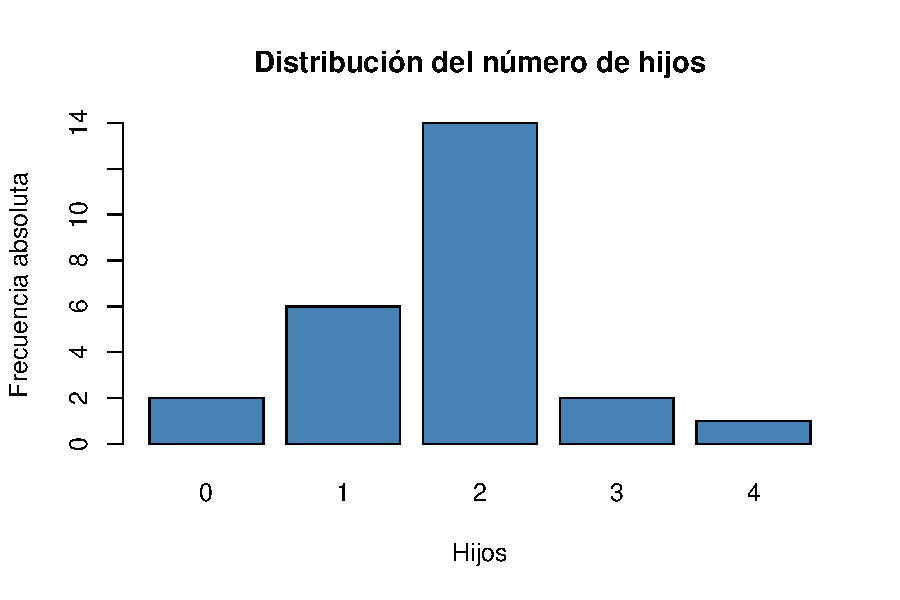
\includegraphics[keepaspectratio]{04-frecuencias-graficos_files/figure-pdf/unnamed-chunk-5-1.pdf}}

\begin{Shaded}
\begin{Highlighting}[]
\CommentTok{\# Diagrama de barras de frecuencias relativas.}
\FunctionTok{barplot}\NormalTok{(fi, }\AttributeTok{col =} \StringTok{"steelblue"}\NormalTok{, }\AttributeTok{main =} \StringTok{"Distribución del número de hijos"}\NormalTok{, }\AttributeTok{xlab =} \StringTok{"Hijos"}\NormalTok{, }\AttributeTok{ylab =} \StringTok{"Frecuencia relativa"}\NormalTok{)}
\end{Highlighting}
\end{Shaded}

  \pandocbounded{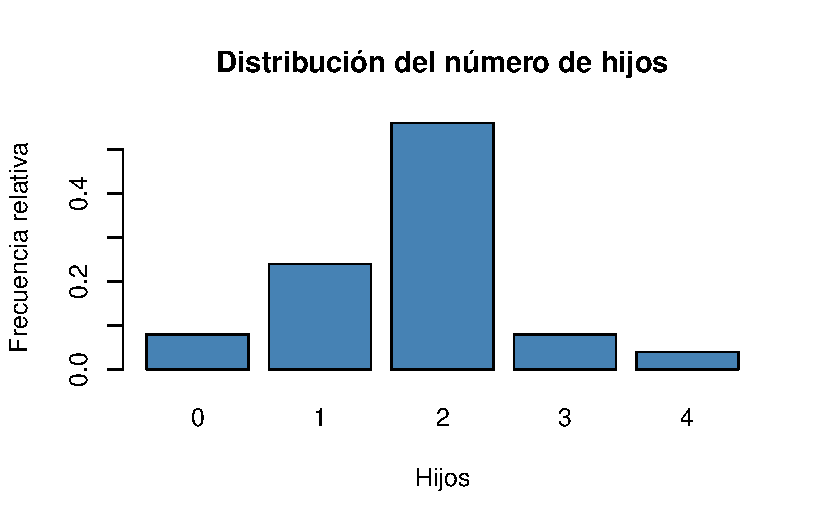
\includegraphics[keepaspectratio]{04-frecuencias-graficos_files/figure-pdf/unnamed-chunk-5-2.pdf}}

\begin{Shaded}
\begin{Highlighting}[]
\CommentTok{\# Diagrama de barras de frecuencias absolutas acumuladas.}
\FunctionTok{barplot}\NormalTok{(Ni, }\AttributeTok{col =} \StringTok{"steelblue"}\NormalTok{, }\AttributeTok{main =} \StringTok{"Distribución acumulada del número de hijos"}\NormalTok{, }\AttributeTok{xlab =} \StringTok{"Hijos"}\NormalTok{, }\AttributeTok{ylab =} \StringTok{"Frecuencia absoluta acumulada"}\NormalTok{)}
\end{Highlighting}
\end{Shaded}

  \pandocbounded{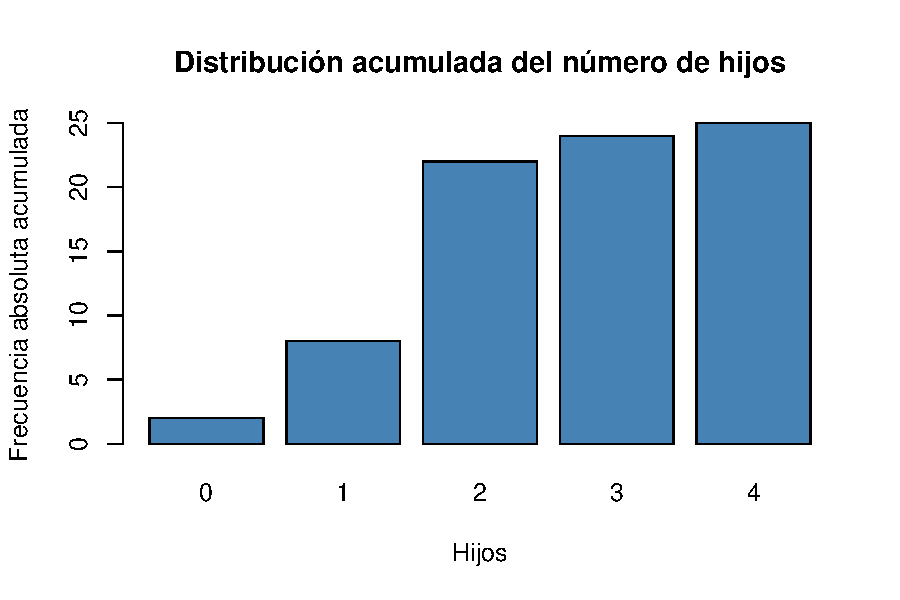
\includegraphics[keepaspectratio]{04-frecuencias-graficos_files/figure-pdf/unnamed-chunk-5-3.pdf}}

\begin{Shaded}
\begin{Highlighting}[]
\CommentTok{\# Diagrama de barras de frecuencias relativas acumuladas.}
\FunctionTok{barplot}\NormalTok{(Fi, }\AttributeTok{col =} \StringTok{"steelblue"}\NormalTok{, }\AttributeTok{main =} \StringTok{"Distribución acumulada del número de hijos"}\NormalTok{, }\AttributeTok{xlab =} \StringTok{"Hijos"}\NormalTok{, }\AttributeTok{ylab =} \StringTok{"Frecuencia relativa acumulada"}\NormalTok{)}
\end{Highlighting}
\end{Shaded}

  \pandocbounded{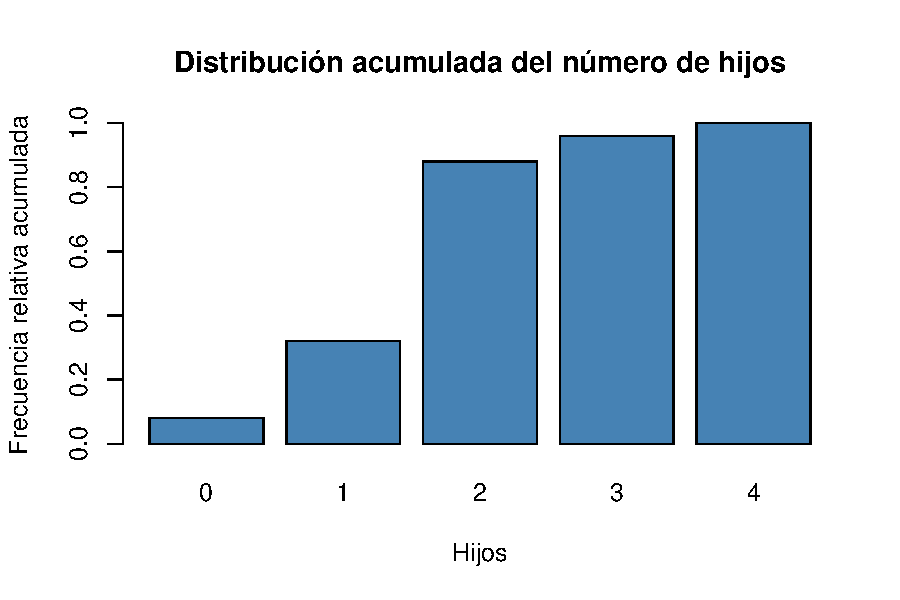
\includegraphics[keepaspectratio]{04-frecuencias-graficos_files/figure-pdf/unnamed-chunk-5-4.pdf}}

  \section{tidyverse}

  Para dibujar un diagrama de barras podemos usar la función
  \href{https://aprendeconalf.es/manual-r/07-graficos.html\#diagramas-de-barras}{\texttt{geom\_bar}}
  del paquete \texttt{ggplot2} de \texttt{tidyverse}. Esta función
  calcula automaticamente las frecuencias absolutas de la columna
  indicada en la dimensión \texttt{x} para barras horizontles o
  \texttt{y} para barras verticales.

  Parámetros:

  \begin{itemize}
  \tightlist
  \item
    color: color del borde de las barras.
  \item
    fill: color de relleno de las barras.
  \item
    width: anchura de las barras (valor entre 0 y 1).
  \end{itemize}

  Para dibujar el diagrama de barras de frecuencias relativas o
  acumuladas, se le pude pasar como parámetro la función
  \href{https://ggplot2.tidyverse.org/reference/geom_bar.html}{\texttt{after\_stat}}
  a la dimensión \texttt{y}:

  \begin{itemize}
  \tightlist
  \item
    \texttt{after\_stat(count/sum(count))}: para las frecuencias
    relativas.
  \item
    \texttt{after\_stat(cumsum(count))}: para las frecuencias absolutas
    acumuladas.
  \item
    \texttt{after\_stat(cumsum(count)/sum(count))}: para las frecuencias
    relativas acumuladas.
  \end{itemize}

\begin{Shaded}
\begin{Highlighting}[]
\CommentTok{\# Diagrama de barras de frecuencias absolutas}
\CommentTok{\# Añadimos la variable a la dimensión x.}
\NormalTok{df }\SpecialCharTok{|\textgreater{}} \FunctionTok{ggplot}\NormalTok{(}\FunctionTok{aes}\NormalTok{(}\AttributeTok{x =}\NormalTok{ hijos)) }\SpecialCharTok{+}
    \CommentTok{\# Añadimos la geometría de barras.}
    \FunctionTok{geom\_bar}\NormalTok{(}\AttributeTok{fill =} \StringTok{"steelblue"}\NormalTok{) }\SpecialCharTok{+}
    \CommentTok{\# Añadimos el título y las etiquetas de los ejes. }
    \FunctionTok{labs}\NormalTok{(}\AttributeTok{title =} \StringTok{"Distribución del número de hijos"}\NormalTok{, }\AttributeTok{y =} \StringTok{"Frecuencia absoluta"}\NormalTok{)}
\end{Highlighting}
\end{Shaded}

  \pandocbounded{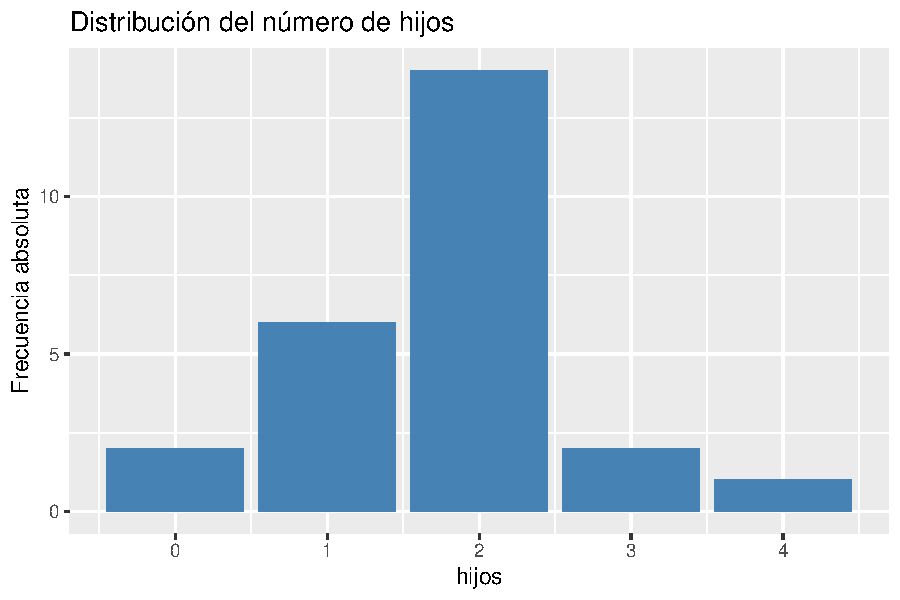
\includegraphics[keepaspectratio]{04-frecuencias-graficos_files/figure-pdf/unnamed-chunk-6-1.pdf}}

\begin{Shaded}
\begin{Highlighting}[]
\CommentTok{\# Diagrama de barras de frecuencias relativas}
\CommentTok{\# Añadimos la variable a la dimensión x.}
\NormalTok{df }\SpecialCharTok{|\textgreater{}} \FunctionTok{ggplot}\NormalTok{(}\FunctionTok{aes}\NormalTok{(}\AttributeTok{x =}\NormalTok{ hijos)) }\SpecialCharTok{+}
    \CommentTok{\# Añadimos la geometría de barras y asignamos a la dimensión y las frecuencias relativas.}
    \FunctionTok{geom\_bar}\NormalTok{(}\FunctionTok{aes}\NormalTok{(}\AttributeTok{y =} \FunctionTok{after\_stat}\NormalTok{(count}\SpecialCharTok{/}\FunctionTok{sum}\NormalTok{(count))), }\AttributeTok{fill =} \StringTok{"steelblue"}\NormalTok{) }\SpecialCharTok{+}
    \CommentTok{\# Añadimos el título y las etiquetas de los ejes.}
    \FunctionTok{labs}\NormalTok{(}\AttributeTok{title =} \StringTok{"Distribución del número de hijos"}\NormalTok{, }\AttributeTok{y =} \StringTok{"Frecuencia relativa"}\NormalTok{)}
\end{Highlighting}
\end{Shaded}

  \pandocbounded{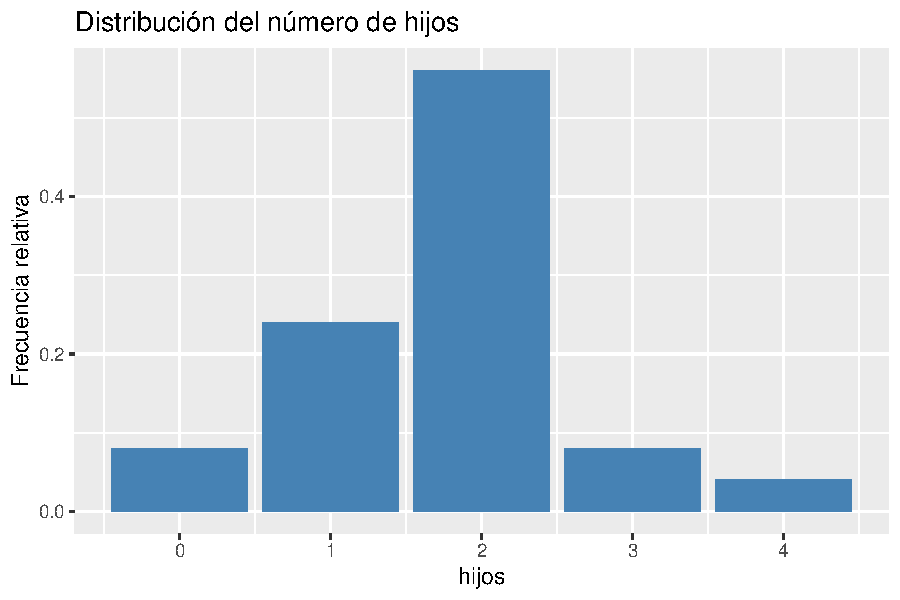
\includegraphics[keepaspectratio]{04-frecuencias-graficos_files/figure-pdf/unnamed-chunk-6-2.pdf}}

\begin{Shaded}
\begin{Highlighting}[]
\CommentTok{\# Diagrama de barras de frecuencias acumuladas}
\CommentTok{\# Añadimos la variable a la dimensión x.}
\NormalTok{df }\SpecialCharTok{|\textgreater{}} \FunctionTok{ggplot}\NormalTok{(}\FunctionTok{aes}\NormalTok{(}\AttributeTok{x =}\NormalTok{ hijos)) }\SpecialCharTok{+}
    \CommentTok{\# Añadimos la geometría de barras y asignamos a la dimensión y las frecuencias absolutas acumuladas.}
    \FunctionTok{geom\_bar}\NormalTok{(}\FunctionTok{aes}\NormalTok{(}\AttributeTok{y =} \FunctionTok{after\_stat}\NormalTok{(}\FunctionTok{cumsum}\NormalTok{(count))), }\AttributeTok{fill =} \StringTok{"steelblue"}\NormalTok{) }\SpecialCharTok{+}
    \CommentTok{\# Añadimos el título y las etiquetas de los ejes.}
    \FunctionTok{labs}\NormalTok{(}\AttributeTok{title =} \StringTok{"Distribución acumulada del número de hijos"}\NormalTok{, }\AttributeTok{y =} \StringTok{"Frecuencia absoluta acumulada"}\NormalTok{)}
\end{Highlighting}
\end{Shaded}

  \pandocbounded{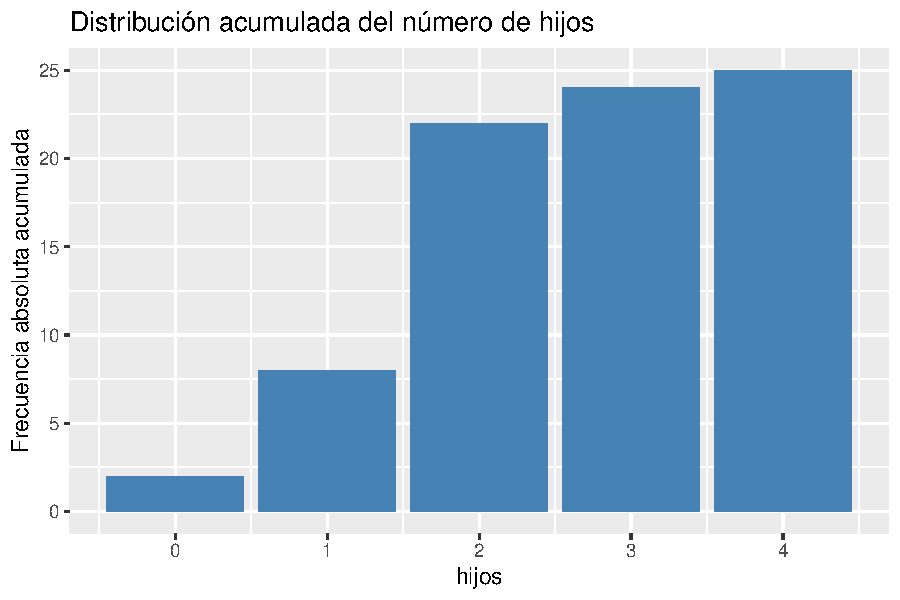
\includegraphics[keepaspectratio]{04-frecuencias-graficos_files/figure-pdf/unnamed-chunk-6-3.pdf}}

\begin{Shaded}
\begin{Highlighting}[]
\CommentTok{\# Diagrama de barras de frecuencias acumuladas}
\CommentTok{\# Añadimos la variable a la dimensión x.}
\NormalTok{df }\SpecialCharTok{|\textgreater{}} \FunctionTok{ggplot}\NormalTok{(}\FunctionTok{aes}\NormalTok{(}\AttributeTok{x =}\NormalTok{ hijos)) }\SpecialCharTok{+}
    \CommentTok{\# Añadimos la geometría de barras y asignamos a la dimensión y las frecuencias relativas acumuladas.}
    \FunctionTok{geom\_bar}\NormalTok{(}\FunctionTok{aes}\NormalTok{(}\AttributeTok{y =} \FunctionTok{after\_stat}\NormalTok{(}\FunctionTok{cumsum}\NormalTok{(count)}\SpecialCharTok{/}\FunctionTok{sum}\NormalTok{(count))), }\AttributeTok{fill =} \StringTok{"steelblue"}\NormalTok{) }\SpecialCharTok{+}
    \CommentTok{\# Añadimos el título y las etiquetas de los ejes.}
    \FunctionTok{labs}\NormalTok{(}\AttributeTok{title =} \StringTok{"Distribución acumulada del número de hijos"}\NormalTok{, }\AttributeTok{y =} \StringTok{"Frecuencia relativa acumulada"}\NormalTok{)}
\end{Highlighting}
\end{Shaded}

  \pandocbounded{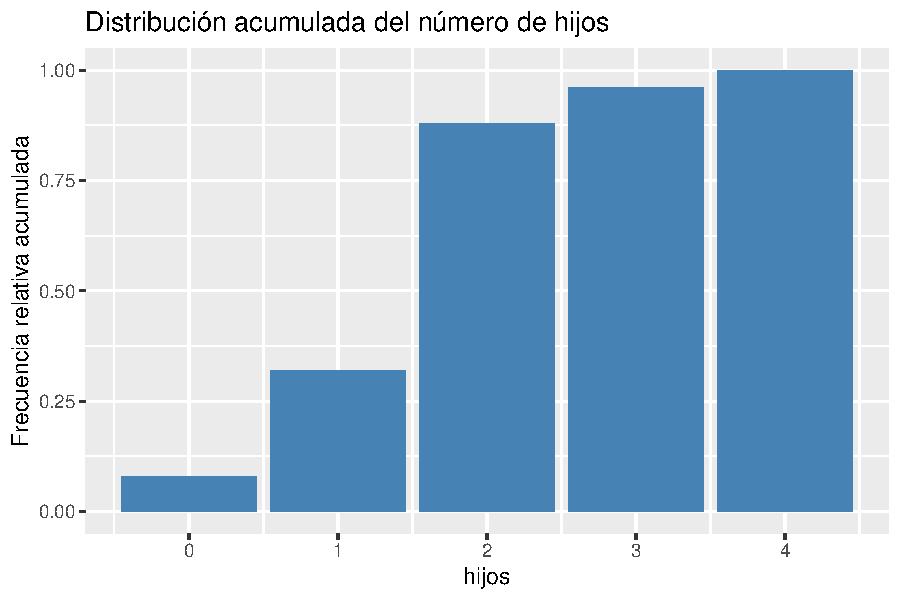
\includegraphics[keepaspectratio]{04-frecuencias-graficos_files/figure-pdf/unnamed-chunk-6-4.pdf}}

  \end{tcolorbox}
\item
  Dibujar el polígono de frecuencias relativas.

  \begin{tcolorbox}[enhanced jigsaw, breakable, leftrule=.75mm, toptitle=1mm, rightrule=.15mm, opacitybacktitle=0.6, left=2mm, colframe=quarto-callout-tip-color-frame, titlerule=0mm, toprule=.15mm, opacityback=0, bottomtitle=1mm, coltitle=black, colbacktitle=quarto-callout-tip-color!10!white, title=\textcolor{quarto-callout-tip-color}{\faLightbulb}\hspace{0.5em}{Solución}, arc=.35mm, bottomrule=.15mm, colback=white]

  \section{Base}

  Para dibujar el polígono de frecuencias podemos usar la función
  \href{https://www.rdocumentation.org/packages/graphics/versions/3.6.2/topics/plot}{\texttt{plot}}
  del paquete \texttt{graphics}.

  Parámetros:

  \begin{itemize}
  \tightlist
  \item
    \texttt{x}: tabla con las frecuencias.
  \item
    \texttt{type}: tipo de gráfico. Para un polígono de frecuencias se
    usa \texttt{"l"} (línea).
  \item
    \texttt{col}: color de la línea.
  \item
    \texttt{main}: título del gráfico.
  \item
    \texttt{xlab}: etiqueta del eje x.
  \item
    \texttt{ylab}: etiqueta del eje y.
  \end{itemize}

\begin{Shaded}
\begin{Highlighting}[]
\CommentTok{\# Frecuencias relativas.}
\FunctionTok{plot}\NormalTok{(fi, }\AttributeTok{type =} \StringTok{"l"}\NormalTok{, }\AttributeTok{col =} \StringTok{"steelblue"}\NormalTok{, }\AttributeTok{main =} \StringTok{"Distribución del número de hijos"}\NormalTok{, }\AttributeTok{xlab =} \StringTok{"Hijos"}\NormalTok{, }\AttributeTok{ylab =} \StringTok{"Frecuencia relativa"}\NormalTok{)}
\end{Highlighting}
\end{Shaded}

  \pandocbounded{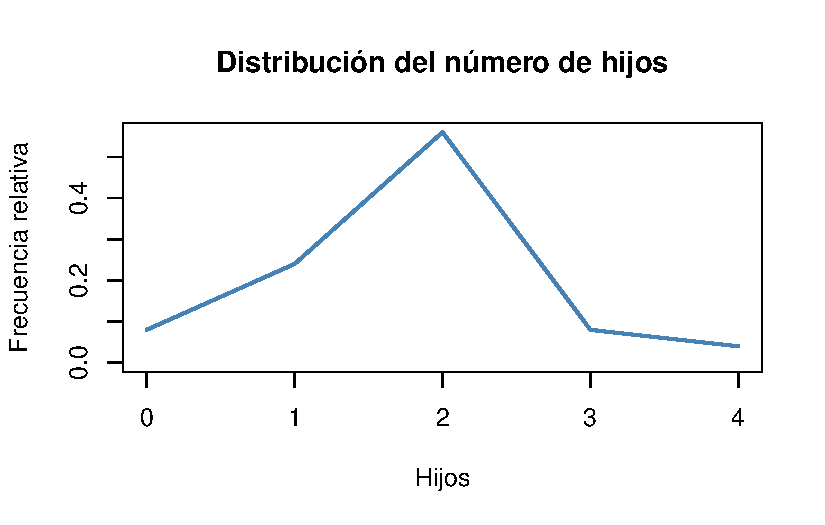
\includegraphics[keepaspectratio]{04-frecuencias-graficos_files/figure-pdf/unnamed-chunk-7-1.pdf}}

  \section{tidyverse}

  Par dibujar el polígono de frecuencias podemos usar la función
  \href{https://aprendeconalf.es/manual-r/07-graficos.html\#diagramas-de-lineas}{\texttt{geom\_line}}
  del paquete \texttt{ggplot2} de \texttt{tidyverse}, que conecta con
  segmentos los puntos con coordenadas pasadas en las dimensiones
  \texttt{x} e \texttt{y}.

  Parámetros:

  \begin{itemize}
  \tightlist
  \item
    \texttt{col}: color de la línea.
  \item
    \texttt{size}: grosor de la línea.
  \item
    \texttt{linetype}: tipo de línea (por ejemplo, ``solid'',
    ``dashed'', ``dotted'').
  \end{itemize}

\begin{Shaded}
\begin{Highlighting}[]
\CommentTok{\# Calculamos las frecuencias absolutas.}
\NormalTok{df }\SpecialCharTok{|\textgreater{}} \FunctionTok{count}\NormalTok{(hijos) }\SpecialCharTok{|\textgreater{}} 
    \CommentTok{\# Añadimos una nueva columna con las frecuencias relativas.}
    \FunctionTok{mutate}\NormalTok{(}\AttributeTok{fi =}\NormalTok{ n}\SpecialCharTok{/}\FunctionTok{sum}\NormalTok{(n)) }\SpecialCharTok{|\textgreater{}}
    \CommentTok{\# Añadimos los hijos a la dimensión x y las frecuencias relativas a la dimensión y.}
    \FunctionTok{ggplot}\NormalTok{(}\FunctionTok{aes}\NormalTok{(}\AttributeTok{x =}\NormalTok{ hijos, }\AttributeTok{y =}\NormalTok{ fi)) }\SpecialCharTok{+}
    \CommentTok{\# Añadimos la geometría de líneas.}
    \FunctionTok{geom\_line}\NormalTok{(}\AttributeTok{col =} \StringTok{"steelblue"}\NormalTok{) }\SpecialCharTok{+}
    \CommentTok{\# Añadimos el título y las etiquetas de los ejes.}
    \FunctionTok{labs}\NormalTok{(}\AttributeTok{title =} \StringTok{"Distribución del número de hijos"}\NormalTok{, }\AttributeTok{y =} \StringTok{"Frecuencia relativa"}\NormalTok{)}
\end{Highlighting}
\end{Shaded}

  \pandocbounded{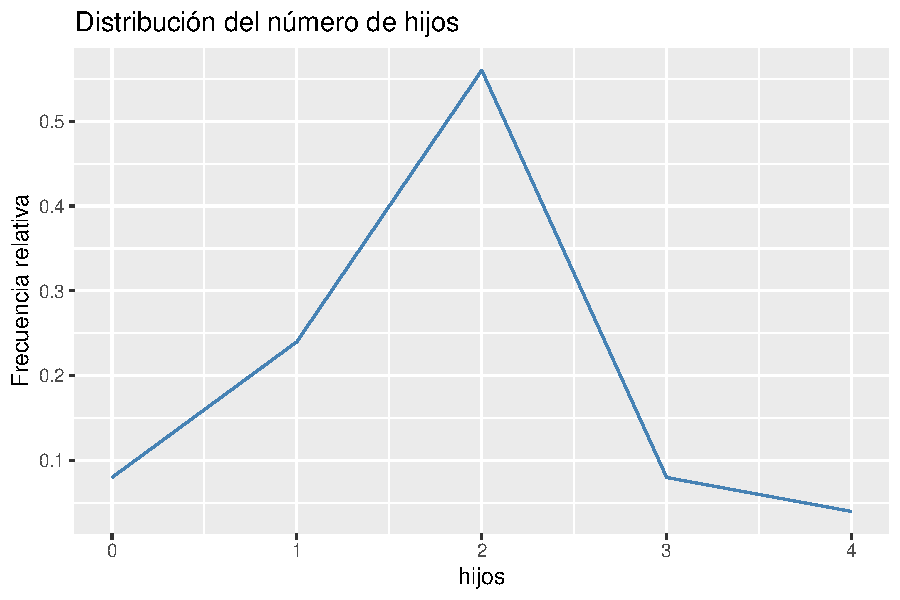
\includegraphics[keepaspectratio]{04-frecuencias-graficos_files/figure-pdf/unnamed-chunk-8-1.pdf}}

  \end{tcolorbox}
\end{enumerate}

\end{exercise}

\begin{exercise}[]\protect\hypertarget{exr-frecuencias-graficos-urgencias}{}\label{exr-frecuencias-graficos-urgencias}

En un hospital se realizó un estudio sobre el número de personas que
ingresaron en urgencias cada día del mes de noviembre. Los datos
observados fueron:

\[
\begin{array}{c}
\mbox{15, 23, 12, 10, 28, 50, 12, 17, 20, 21, 18, 13, 11, 12, 26} \\
\mbox{30, 6, 16, 19, 22, 14, 17, 21, 28, 9, 16, 13, 11, 16, 20}
\end{array}
\]

\begin{enumerate}
\def\labelenumi{\alph{enumi}.}
\item
  Crear un conjunto de datos con la variable \texttt{urgencias}.

  \begin{tcolorbox}[enhanced jigsaw, breakable, leftrule=.75mm, toptitle=1mm, rightrule=.15mm, opacitybacktitle=0.6, left=2mm, colframe=quarto-callout-tip-color-frame, titlerule=0mm, toprule=.15mm, opacityback=0, bottomtitle=1mm, coltitle=black, colbacktitle=quarto-callout-tip-color!10!white, title=\textcolor{quarto-callout-tip-color}{\faLightbulb}\hspace{0.5em}{Solución}, arc=.35mm, bottomrule=.15mm, colback=white]

  \section{Base}

\begin{Shaded}
\begin{Highlighting}[]
\NormalTok{df }\OtherTok{\textless{}{-}} \FunctionTok{data.frame}\NormalTok{(}\AttributeTok{urgencias =} \FunctionTok{c}\NormalTok{(}\DecValTok{15}\NormalTok{, }\DecValTok{23}\NormalTok{, }\DecValTok{12}\NormalTok{, }\DecValTok{10}\NormalTok{, }\DecValTok{28}\NormalTok{, }\DecValTok{50}\NormalTok{, }\DecValTok{12}\NormalTok{, }\DecValTok{17}\NormalTok{, }\DecValTok{20}\NormalTok{, }\DecValTok{21}\NormalTok{, }\DecValTok{18}\NormalTok{, }\DecValTok{13}\NormalTok{, }\DecValTok{11}\NormalTok{, }\DecValTok{12}\NormalTok{, }\DecValTok{26}\NormalTok{, }\DecValTok{30}\NormalTok{, }\DecValTok{6}\NormalTok{, }\DecValTok{16}\NormalTok{, }\DecValTok{19}\NormalTok{, }\DecValTok{22}\NormalTok{, }\DecValTok{14}\NormalTok{, }\DecValTok{17}\NormalTok{, }\DecValTok{21}\NormalTok{, }\DecValTok{28}\NormalTok{, }\DecValTok{9}\NormalTok{, }\DecValTok{16}\NormalTok{, }\DecValTok{13}\NormalTok{, }\DecValTok{11}\NormalTok{, }\DecValTok{16}\NormalTok{, }\DecValTok{20}\NormalTok{))}
\end{Highlighting}
\end{Shaded}

  \section{tidyverse}

\begin{Shaded}
\begin{Highlighting}[]
\FunctionTok{library}\NormalTok{(tidyverse)}
\NormalTok{df }\OtherTok{\textless{}{-}} \FunctionTok{tibble}\NormalTok{(}\AttributeTok{urgencias =} \FunctionTok{c}\NormalTok{(}\DecValTok{15}\NormalTok{, }\DecValTok{23}\NormalTok{, }\DecValTok{12}\NormalTok{, }\DecValTok{10}\NormalTok{, }\DecValTok{28}\NormalTok{, }\DecValTok{50}\NormalTok{, }\DecValTok{12}\NormalTok{, }\DecValTok{17}\NormalTok{, }\DecValTok{20}\NormalTok{, }\DecValTok{21}\NormalTok{, }\DecValTok{18}\NormalTok{, }\DecValTok{13}\NormalTok{, }\DecValTok{11}\NormalTok{, }\DecValTok{12}\NormalTok{, }\DecValTok{26}\NormalTok{, }\DecValTok{30}\NormalTok{, }\DecValTok{6}\NormalTok{, }\DecValTok{16}\NormalTok{, }\DecValTok{19}\NormalTok{, }\DecValTok{22}\NormalTok{, }\DecValTok{14}\NormalTok{, }\DecValTok{17}\NormalTok{, }\DecValTok{21}\NormalTok{, }\DecValTok{28}\NormalTok{, }\DecValTok{9}\NormalTok{, }\DecValTok{16}\NormalTok{, }\DecValTok{13}\NormalTok{, }\DecValTok{11}\NormalTok{, }\DecValTok{16}\NormalTok{, }\DecValTok{20}\NormalTok{))}
\end{Highlighting}
\end{Shaded}

  \end{tcolorbox}
\item
  Dibujar el diagrama de cajas. ¿Existe algún dato atípico? En el caso
  de que exista, eliminarlo y proceder con los siguientes apartados.

  \begin{tcolorbox}[enhanced jigsaw, breakable, leftrule=.75mm, toptitle=1mm, rightrule=.15mm, opacitybacktitle=0.6, left=2mm, colframe=quarto-callout-tip-color-frame, titlerule=0mm, toprule=.15mm, opacityback=0, bottomtitle=1mm, coltitle=black, colbacktitle=quarto-callout-tip-color!10!white, title=\textcolor{quarto-callout-tip-color}{\faLightbulb}\hspace{0.5em}{Solución}, arc=.35mm, bottomrule=.15mm, colback=white]

  \section{Base}

  Para dibujar un diagrama de caja y bigotes podemos usar la función
  \href{https://www.rdocumentation.org/packages/graphics/versions/3.6.2/topics/boxplot}{\texttt{boxplot}}
  del paquete \texttt{graphics}.

  Parámetros:

  \begin{itemize}
  \tightlist
  \item
    \texttt{x}: vector con las alturas de las barras.
  \item
    \texttt{col}: color de la caja.
  \item
    \texttt{horizontal}: orientación horizontal de la caja (True o
    False).
  \item
    \texttt{width}: anchura de la caja (valor entre 0 y 1).
  \item
    \texttt{main}: título del gráfico.
  \item
    \texttt{xlab}: etiqueta del eje x.
  \item
    \texttt{ylab}: etiqueta del eje y.
  \end{itemize}

\begin{Shaded}
\begin{Highlighting}[]
\FunctionTok{boxplot}\NormalTok{(df}\SpecialCharTok{$}\NormalTok{urgencias, }\AttributeTok{col =} \StringTok{"steelblue"}\NormalTok{,  }\AttributeTok{horizontal =}\NormalTok{ T, }\AttributeTok{main =} \StringTok{"Distribución del número de urgencias"}\NormalTok{, }\AttributeTok{xlab =} \StringTok{"Número de urgencias"}\NormalTok{)}
\end{Highlighting}
\end{Shaded}

  \pandocbounded{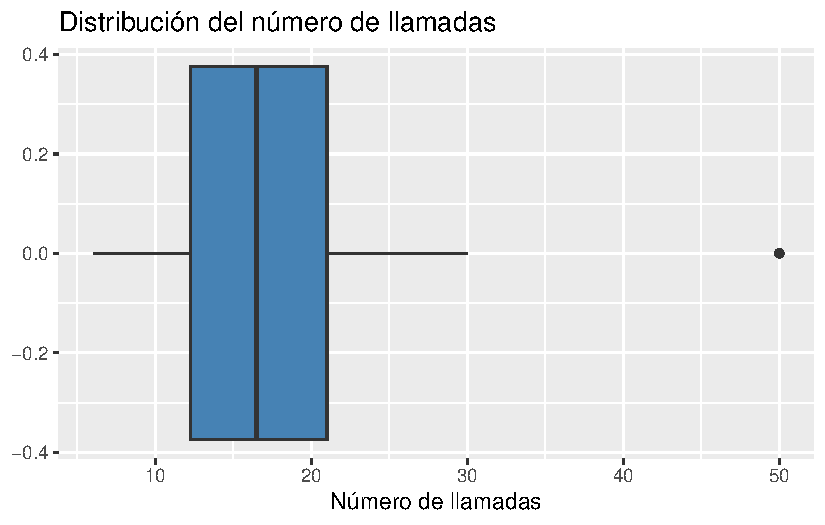
\includegraphics[keepaspectratio]{04-frecuencias-graficos_files/figure-pdf/unnamed-chunk-11-1.pdf}}

  \section{tidyverse}

  Para dibujar un diagrama de caja y bigotes podemos usar la función
  \href{https://aprendeconalf.es/manual-r/07-graficos.html\#diagramas-de-cajas}{\texttt{geom\_boxplot}}
  del paquete \texttt{ggplot2} de \texttt{tidyverse}.

  Parámetros:

  \begin{itemize}
  \tightlist
  \item
    color: color del borde de la caja.
  \item
    fill: color de relleno de la caja.
  \item
    width: anchura de la caja.
  \end{itemize}

\begin{Shaded}
\begin{Highlighting}[]
\CommentTok{\# Añadimos la variable a la dimensión x.}
\NormalTok{df }\SpecialCharTok{|\textgreater{}} \FunctionTok{ggplot}\NormalTok{(}\FunctionTok{aes}\NormalTok{(}\AttributeTok{x =}\NormalTok{ urgencias)) }\SpecialCharTok{+}
    \CommentTok{\# Añadimos la geometría de cajas.}
    \FunctionTok{geom\_boxplot}\NormalTok{(}\AttributeTok{fill =} \StringTok{"steelblue"}\NormalTok{) }\SpecialCharTok{+}
    \CommentTok{\# Eliminamos las marcas del eje y.}
    \FunctionTok{scale\_y\_continuous}\NormalTok{(}\AttributeTok{breaks =} \ConstantTok{NULL}\NormalTok{) }\SpecialCharTok{+}
    \CommentTok{\# Añadimos el título y las etiquetas.}
    \FunctionTok{labs}\NormalTok{(}\AttributeTok{title =} \StringTok{"Distribución del número de urgencias"}\NormalTok{, }\AttributeTok{x =} \StringTok{"Número de urgencias"}\NormalTok{)}
\end{Highlighting}
\end{Shaded}

  \pandocbounded{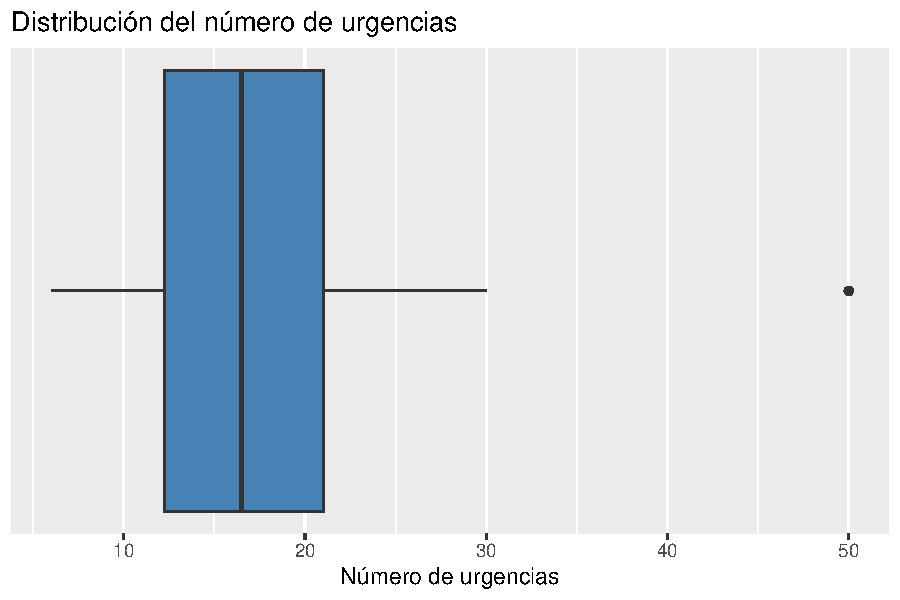
\includegraphics[keepaspectratio]{04-frecuencias-graficos_files/figure-pdf/unnamed-chunk-12-1.pdf}}

  Hay un día con 50 urgencias, que es un valor atípico en comparación
  con el resto de días.

  \section{Base}

  Con las funciones del paquete \texttt{base} de R.

\begin{Shaded}
\begin{Highlighting}[]
\CommentTok{\# Eliminamos el dato atípico.}
\NormalTok{df }\OtherTok{\textless{}{-}}\NormalTok{ df[df}\SpecialCharTok{$}\NormalTok{urgencias }\SpecialCharTok{!=} \DecValTok{50}\NormalTok{, , drop }\OtherTok{=}\NormalTok{ F]}
\end{Highlighting}
\end{Shaded}

  \section{tidyverse}

  Con la función \texttt{filter} del paquete \texttt{dplyr} de
  \texttt{tidyverse}.

\begin{Shaded}
\begin{Highlighting}[]
\CommentTok{\# Eliminamos el dato atípico.}
\NormalTok{df }\OtherTok{\textless{}{-}} \FunctionTok{filter}\NormalTok{(df, urgencias }\SpecialCharTok{!=} \DecValTok{50}\NormalTok{)}
\end{Highlighting}
\end{Shaded}

  \end{tcolorbox}
\item
  Construir la tabla de frecuencias agrupando en 5 clases.

  \begin{tcolorbox}[enhanced jigsaw, breakable, leftrule=.75mm, toptitle=1mm, rightrule=.15mm, opacitybacktitle=0.6, left=2mm, colframe=quarto-callout-tip-color-frame, titlerule=0mm, toprule=.15mm, opacityback=0, bottomtitle=1mm, coltitle=black, colbacktitle=quarto-callout-tip-color!10!white, title=\textcolor{quarto-callout-tip-color}{\faLightbulb}\hspace{0.5em}{Solución}, arc=.35mm, bottomrule=.15mm, colback=white]

  \section{Base}

  Para agrupar los datos en intervalos se puede utilizar la función
  \href{https://www.rdocumentation.org/packages/base/versions/3.6.2/topics/cut}{\texttt{cut}}
  del paquete base de R.

  Parámetros:

  \begin{itemize}
  \tightlist
  \item
    \texttt{breaks}: número de intervalos o un vector con los puntos de
    corte de los intervalos.
  \end{itemize}

  Para contar las frecuencias absolutas y relativas podemos usar las
  funciones
  \href{https://www.rdocumentation.org/packages/base/versions/3.6.2/topics/table}{\texttt{table}},
  y
  \href{https://www.rdocumentation.org/packages/base/versions/3.6.2/topics/prop.table}{\texttt{prop.table}}
  respectivamente.

  Posteriormente, para obtener las frecuencias acumuladas se puede usar
  la función
  \href{https://www.rdocumentation.org/packages/base/versions/3.6.2/topics/cumsum}{\texttt{cumsum}}
  aplicada a las frecuencias absolutas y relativas.

\begin{Shaded}
\begin{Highlighting}[]
\FunctionTok{library}\NormalTok{(knitr)}
\CommentTok{\# Calculamos las frecuencias absolutas agrupando en 5 clases desde 5 hasta 30.}
\NormalTok{ni }\OtherTok{\textless{}{-}} \FunctionTok{table}\NormalTok{(}\FunctionTok{cut}\NormalTok{(df}\SpecialCharTok{$}\NormalTok{urgencias, }\AttributeTok{breaks =} \FunctionTok{seq}\NormalTok{(}\DecValTok{5}\NormalTok{, }\DecValTok{30}\NormalTok{, }\DecValTok{5}\NormalTok{)))}
\CommentTok{\# Frecuencias relativas}
\NormalTok{fi }\OtherTok{\textless{}{-}} \FunctionTok{prop.table}\NormalTok{(ni)}
\CommentTok{\# Frecuencias acumuladas.}
\NormalTok{Ni }\OtherTok{\textless{}{-}} \FunctionTok{cumsum}\NormalTok{(ni)}
\CommentTok{\# Frecuencias relativas acumuladas.}
\NormalTok{Fi }\OtherTok{\textless{}{-}} \FunctionTok{cumsum}\NormalTok{(fi)}
\CommentTok{\# Creación de un data frame con las frecuencias.}
\NormalTok{tabla\_frec }\OtherTok{\textless{}{-}} \FunctionTok{cbind}\NormalTok{(ni, fi, Ni, Fi)}
\FunctionTok{kable}\NormalTok{(tabla\_frec)}
\end{Highlighting}
\end{Shaded}

  \begin{longtable}[]{@{}lrrrr@{}}
  \toprule\noalign{}
  & ni & fi & Ni & Fi \\
  \midrule\noalign{}
  \endhead
  \bottomrule\noalign{}
  \endlastfoot
  (5,10{]} & 3 & 0.1034483 & 3 & 0.1034483 \\
  (10,15{]} & 9 & 0.3103448 & 12 & 0.4137931 \\
  (15,20{]} & 9 & 0.3103448 & 21 & 0.7241379 \\
  (20,25{]} & 4 & 0.1379310 & 25 & 0.8620690 \\
  (25,30{]} & 4 & 0.1379310 & 29 & 1.0000000 \\
  \end{longtable}

  \section{tidyverse}

  Para agrupar los datos en intervalos se puede utilizar la función
  \href{https://www.rdocumentation.org/packages/base/versions/3.6.2/topics/cut}{\texttt{cut}}
  del paquete base de R y añadir una nueva columna al data frame con la
  clase a la que pertenece cada individuo con la función
  \texttt{mutate}.

  Después, podemos obtener la tabla de frecuencias podemos usar la
  función
  \href{https://aprendeconalf.es/manual-r/06-preprocesamiento.html\#conteo-del-n\%C3\%BAmero-de-observaciones}{\texttt{count}}
  del paquete \texttt{dplyr} de \texttt{tidyverse}.

  Posteriormente podemos añadir nuevas columnas a la tabla de
  frecuencias mediante la función \texttt{mutate} y fórmulas para
  calcular las frecuencias relativas (\texttt{n/sum(n)}), frecuencias
  absolutas acumuladas (\texttt{cumsum(n)}) y frecuencias relativas
  acumuladas (\texttt{cumsum(n)/sum(n)}).

\begin{Shaded}
\begin{Highlighting}[]
\FunctionTok{library}\NormalTok{(knitr)}
\CommentTok{\# Añadimos una nueva columna al data frame con la clase a la que pertenece cada individuo.}
\NormalTok{df }\SpecialCharTok{|\textgreater{}} \FunctionTok{mutate}\NormalTok{(}\AttributeTok{urgencias\_int =} \FunctionTok{cut}\NormalTok{(urgencias, }\AttributeTok{breaks =} \FunctionTok{seq}\NormalTok{(}\DecValTok{5}\NormalTok{, }\DecValTok{30}\NormalTok{, }\DecValTok{5}\NormalTok{))) }\SpecialCharTok{|\textgreater{}} 
    \CommentTok{\# Calculamos la tabla de frecuencias absolutas.}
    \FunctionTok{count}\NormalTok{(urgencias\_int) }\SpecialCharTok{|\textgreater{}}
    \CommentTok{\# Añadimos nuevas columnas con la frecuencia relativa, acumulada y relativa acumulada.}
    \FunctionTok{mutate}\NormalTok{(}\AttributeTok{fi =}\NormalTok{ n}\SpecialCharTok{/}\FunctionTok{sum}\NormalTok{(n), }\AttributeTok{Ni =} \FunctionTok{cumsum}\NormalTok{(n), }\AttributeTok{Fi =} \FunctionTok{cumsum}\NormalTok{(n)}\SpecialCharTok{/}\FunctionTok{sum}\NormalTok{(n)) }\SpecialCharTok{|\textgreater{}}
    \FunctionTok{kable}\NormalTok{()}
\end{Highlighting}
\end{Shaded}

  \begin{longtable}[]{@{}lrrrr@{}}
  \toprule\noalign{}
  urgencias\_int & n & fi & Ni & Fi \\
  \midrule\noalign{}
  \endhead
  \bottomrule\noalign{}
  \endlastfoot
  (5,10{]} & 3 & 0.1034483 & 3 & 0.1034483 \\
  (10,15{]} & 9 & 0.3103448 & 12 & 0.4137931 \\
  (15,20{]} & 9 & 0.3103448 & 21 & 0.7241379 \\
  (20,25{]} & 4 & 0.1379310 & 25 & 0.8620690 \\
  (25,30{]} & 4 & 0.1379310 & 29 & 1.0000000 \\
  \end{longtable}

  \end{tcolorbox}
\item
  Dibujar el histograma de frecuencias absolutas, relativas, absolutas
  acumuladas y relativas acumuladas correspondiente a la tabla anterior.

  \begin{tcolorbox}[enhanced jigsaw, breakable, leftrule=.75mm, toptitle=1mm, rightrule=.15mm, opacitybacktitle=0.6, left=2mm, colframe=quarto-callout-tip-color-frame, titlerule=0mm, toprule=.15mm, opacityback=0, bottomtitle=1mm, coltitle=black, colbacktitle=quarto-callout-tip-color!10!white, title=\textcolor{quarto-callout-tip-color}{\faLightbulb}\hspace{0.5em}{Solución}, arc=.35mm, bottomrule=.15mm, colback=white]

  \section{Base}

  Para dibujar un histograma de frecuencias absolutas podemos usar la
  función
  \href{https://www.rdocumentation.org/packages/graphics/versions/3.6.2/topics/hist}{\texttt{hist}}
  del paquete \texttt{graphics}.

  Parámetros:

  \begin{itemize}
  \tightlist
  \item
    \texttt{breaks}: Un vector con los puntos de corte de los intervalos
    de las barras.
  \item
    \texttt{col}: color de las barras.
  \item
    \texttt{main}: título del gráfico.
  \item
    \texttt{xlab}: etiqueta del eje x.
  \item
    \texttt{ylab}: etiqueta del eje y.
  \end{itemize}

  Después se puede cambiar el campo \texttt{counts} del histograma para
  indicar la altura de las barras. Para volver a dibujar el histograma,
  una vez modificadas las alturas de las barras, se tiene que utilizar
  la función \texttt{plot} del paquete \texttt{graphics}.

\begin{Shaded}
\begin{Highlighting}[]
\CommentTok{\# Histograma de frecuencias absolutas.}
\NormalTok{histo }\OtherTok{\textless{}{-}} \FunctionTok{hist}\NormalTok{(df}\SpecialCharTok{$}\NormalTok{urgencias, }\AttributeTok{breaks =} \FunctionTok{seq}\NormalTok{(}\DecValTok{5}\NormalTok{, }\DecValTok{30}\NormalTok{, }\DecValTok{5}\NormalTok{), }\AttributeTok{col =} \StringTok{"steelblue"}\NormalTok{, }\AttributeTok{main =} \StringTok{"Distribución del número de urgencias"}\NormalTok{, }\AttributeTok{xlab =} \StringTok{"urgencias"}\NormalTok{, }\AttributeTok{ylab =} \StringTok{"Frecuencia absoluta"}\NormalTok{)}
\end{Highlighting}
\end{Shaded}

  \pandocbounded{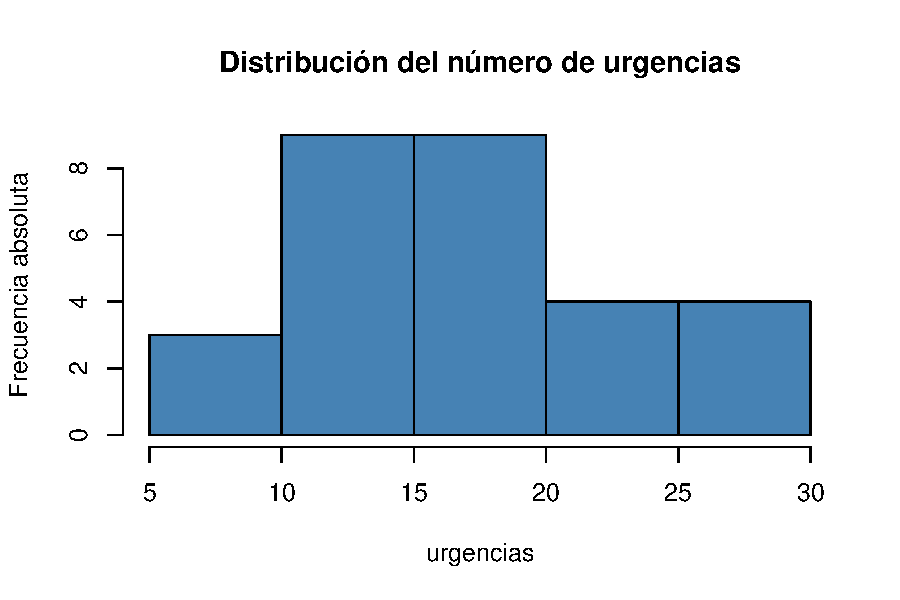
\includegraphics[keepaspectratio]{04-frecuencias-graficos_files/figure-pdf/unnamed-chunk-17-1.pdf}}

\begin{Shaded}
\begin{Highlighting}[]
\NormalTok{ni }\OtherTok{\textless{}{-}}\NormalTok{ histo}\SpecialCharTok{$}\NormalTok{counts}

\CommentTok{\# Histograma de frecuencias relativas.}
\CommentTok{\# Modificamos el campo counts del histograma para que contenga las frecuencias relativas.}
\NormalTok{histo}\SpecialCharTok{$}\NormalTok{counts }\OtherTok{\textless{}{-}}\NormalTok{ ni}\SpecialCharTok{/}\FunctionTok{sum}\NormalTok{(ni)}
\FunctionTok{plot}\NormalTok{(histo, }\AttributeTok{col =} \StringTok{"steelblue"}\NormalTok{, }\AttributeTok{main =} \StringTok{"Distribución del número de urgencias"}\NormalTok{, }\AttributeTok{xlab =} \StringTok{"urgencias"}\NormalTok{, }\AttributeTok{ylab =} \StringTok{"Frecuencia relativa"}\NormalTok{)}
\end{Highlighting}
\end{Shaded}

  \pandocbounded{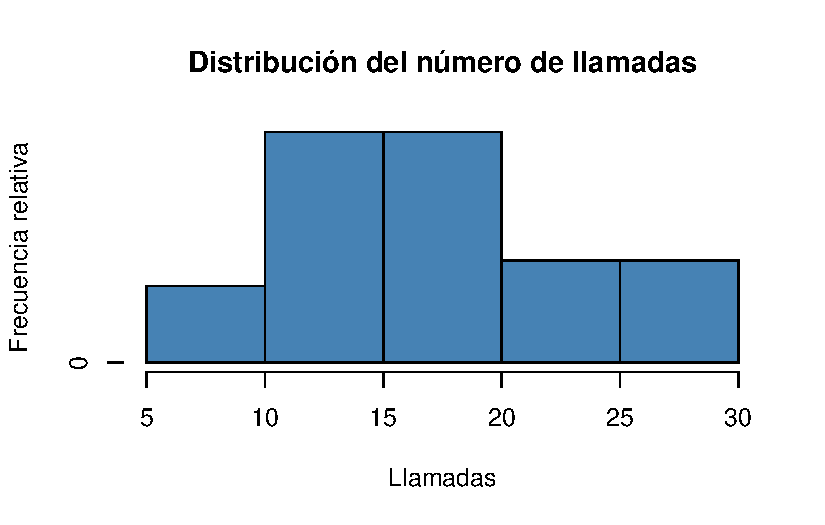
\includegraphics[keepaspectratio]{04-frecuencias-graficos_files/figure-pdf/unnamed-chunk-17-2.pdf}}

\begin{Shaded}
\begin{Highlighting}[]
\CommentTok{\# Histograma de frecuencias absolutas acumuladas.}
\CommentTok{\# Modificamos el campo counts del histograma para que contenga las frecuencias absolutas acumuladas.}
\NormalTok{histo}\SpecialCharTok{$}\NormalTok{counts }\OtherTok{\textless{}{-}} \FunctionTok{cumsum}\NormalTok{(ni)}
\FunctionTok{plot}\NormalTok{(histo, }\AttributeTok{col =} \StringTok{"steelblue"}\NormalTok{, }\AttributeTok{main =} \StringTok{"Distribución acumulada del número de urgencias"}\NormalTok{, }\AttributeTok{xlab =} \StringTok{"urgencias"}\NormalTok{, }\AttributeTok{ylab =} \StringTok{"Frecuencia absoluta acumulada"}\NormalTok{)}
\end{Highlighting}
\end{Shaded}

  \pandocbounded{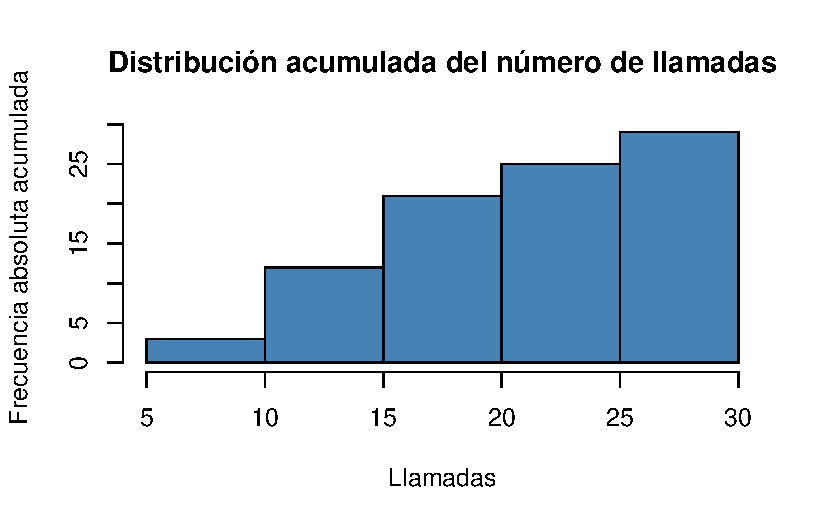
\includegraphics[keepaspectratio]{04-frecuencias-graficos_files/figure-pdf/unnamed-chunk-17-3.pdf}}

\begin{Shaded}
\begin{Highlighting}[]
\CommentTok{\# Histograma de frecuencias relativas acumuladas.}
\CommentTok{\# Modificamos el campo counts del histograma para que contenga las frecuencias relativas.}
\NormalTok{histo}\SpecialCharTok{$}\NormalTok{counts }\OtherTok{\textless{}{-}} \FunctionTok{cumsum}\NormalTok{(ni)}\SpecialCharTok{/}\FunctionTok{sum}\NormalTok{(ni)}
\FunctionTok{plot}\NormalTok{(histo, }\AttributeTok{col =} \StringTok{"steelblue"}\NormalTok{, }\AttributeTok{main =} \StringTok{"Distribución acumulada del número de urgencias"}\NormalTok{, }\AttributeTok{xlab =} \StringTok{"urgencias"}\NormalTok{, }\AttributeTok{ylab =} \StringTok{"Frecuencia relativa acumulada"}\NormalTok{, )}
\end{Highlighting}
\end{Shaded}

  \pandocbounded{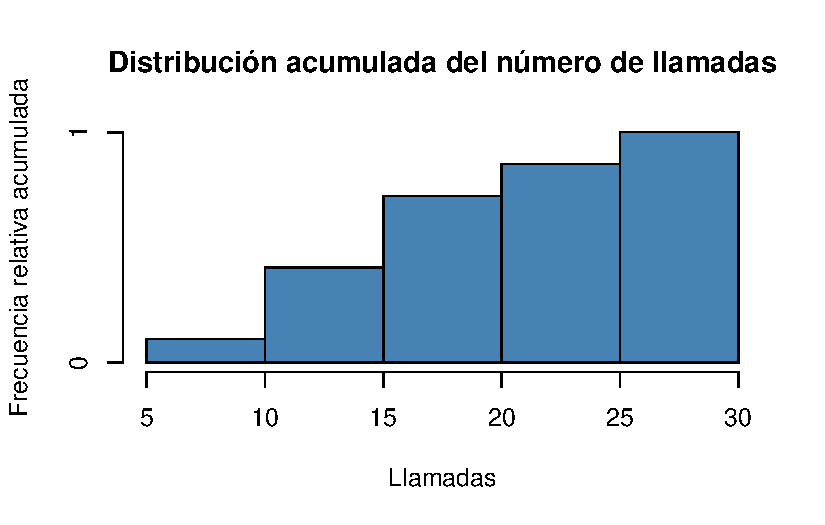
\includegraphics[keepaspectratio]{04-frecuencias-graficos_files/figure-pdf/unnamed-chunk-17-4.pdf}}

  \section{tidyverse}

  Para dibujar un histograma podemos usar la
  función\href{https://aprendeconalf.es/manual-r/07-graficos.html\#histogramas}{\texttt{geom\_histogram}}
  del paquete \texttt{ggplot2} de \texttt{tidyverse}.

  Parámetros:

  \begin{itemize}
  \tightlist
  \item
    \texttt{breaks}: Un vector con los puntos de corte de los intervalos
    de las barras.
  \item
    \texttt{color}: Color del borde de las barras.
  \item
    \texttt{fill}: Color de relleno de las barras.
  \end{itemize}

  Para dibujar el histograma de frecuencias relativas o acumuladas, se
  le pude pasar como parámetro la función
  \href{https://ggplot2.tidyverse.org/reference/geom_bar.html}{\texttt{after\_stat}}
  a la dimesión \texttt{y}.

  \begin{itemize}
  \tightlist
  \item
    \texttt{after\_stat(count/sum(count))}: para las frecuencias
    relativas.
  \item
    \texttt{after\_stat(cumsum(count))}: para las frecuencias absolutas
    acumuladas.
  \item
    \texttt{after\_stat(cumsum(count)/sum(count))}: para las frecuencias
    relativas acumuladas.
  \end{itemize}

\begin{Shaded}
\begin{Highlighting}[]
\CommentTok{\# Histograma de frecuencias absolutas}
\CommentTok{\# Añadimos la variable a la dimensión x.}
\NormalTok{df }\SpecialCharTok{|\textgreater{}} \FunctionTok{ggplot}\NormalTok{(}\FunctionTok{aes}\NormalTok{(}\AttributeTok{x =}\NormalTok{ urgencias)) }\SpecialCharTok{+}
    \CommentTok{\# Añadimos la geometría de histograma creando clases de amplitud 5 desde 5 hasta 30.}
    \FunctionTok{geom\_histogram}\NormalTok{(}\AttributeTok{breaks =} \FunctionTok{seq}\NormalTok{(}\DecValTok{5}\NormalTok{, }\DecValTok{30}\NormalTok{, }\DecValTok{5}\NormalTok{), }\AttributeTok{fill =} \StringTok{"steelblue"}\NormalTok{, }\AttributeTok{col =} \StringTok{"white"}\NormalTok{) }\SpecialCharTok{+} 
    \CommentTok{\# Añadimos el título y las etiquetas de los ejes.}
    \FunctionTok{labs}\NormalTok{(}\AttributeTok{title =} \StringTok{"Distribución del número de urgencias"}\NormalTok{, }\AttributeTok{x =} \StringTok{"Número de urgencias"}\NormalTok{, }\AttributeTok{y =} \StringTok{"Frecuencia absoluta"}\NormalTok{)}
\end{Highlighting}
\end{Shaded}

  \pandocbounded{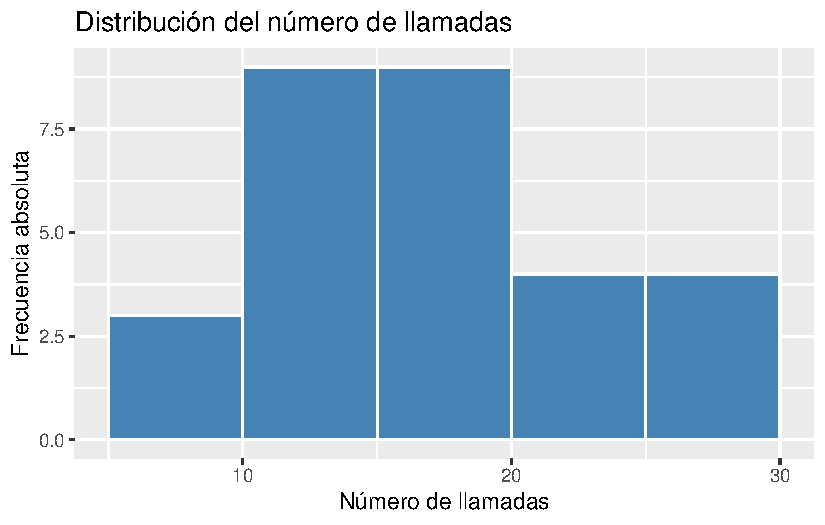
\includegraphics[keepaspectratio]{04-frecuencias-graficos_files/figure-pdf/unnamed-chunk-18-1.pdf}}

\begin{Shaded}
\begin{Highlighting}[]
\CommentTok{\# Histograma de frecuencias relativas}
\CommentTok{\# Añadimos la variable a la dimensión x.}
\NormalTok{df }\SpecialCharTok{|\textgreater{}} \FunctionTok{ggplot}\NormalTok{(}\FunctionTok{aes}\NormalTok{(}\AttributeTok{x =}\NormalTok{ urgencias)) }\SpecialCharTok{+}
    \CommentTok{\# Añadimos la geometría de histograma y asignamos a la dimensión y las frecuencias relativas.}
    \FunctionTok{geom\_histogram}\NormalTok{(}\FunctionTok{aes}\NormalTok{(}\AttributeTok{y =} \FunctionTok{after\_stat}\NormalTok{(count}\SpecialCharTok{/}\FunctionTok{sum}\NormalTok{(count))), }\AttributeTok{breaks =} \FunctionTok{seq}\NormalTok{(}\DecValTok{5}\NormalTok{, }\DecValTok{30}\NormalTok{, }\DecValTok{5}\NormalTok{), }\AttributeTok{fill =} \StringTok{"steelblue"}\NormalTok{, }\AttributeTok{col =} \StringTok{"white"}\NormalTok{) }\SpecialCharTok{+}
    \CommentTok{\# Añadimos el título y las etiquetas de los ejes.}
    \FunctionTok{labs}\NormalTok{(}\AttributeTok{title =} \StringTok{"Distribución del número de urgencias"}\NormalTok{, }\AttributeTok{x =} \StringTok{"Número de urgencias"}\NormalTok{, }\AttributeTok{y =} \StringTok{"Frecuencia relativa"}\NormalTok{)}
\end{Highlighting}
\end{Shaded}

  \pandocbounded{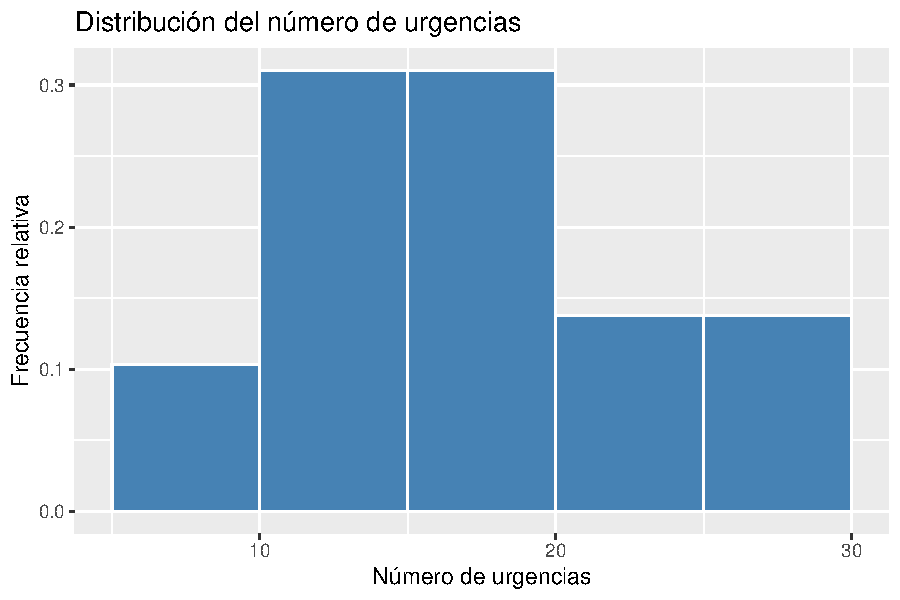
\includegraphics[keepaspectratio]{04-frecuencias-graficos_files/figure-pdf/unnamed-chunk-18-2.pdf}}

\begin{Shaded}
\begin{Highlighting}[]
\CommentTok{\# Histograma de frecuencias acumuladas}
\CommentTok{\# Añadimos la variable a la dimensión x.}
\NormalTok{df }\SpecialCharTok{|\textgreater{}} \FunctionTok{ggplot}\NormalTok{(}\FunctionTok{aes}\NormalTok{(}\AttributeTok{x =}\NormalTok{ urgencias)) }\SpecialCharTok{+}
    \CommentTok{\# Añadimos la geometría de histograma y asignamos a la dimensión y las frecuencias absolutas acumuladas.}
    \FunctionTok{geom\_histogram}\NormalTok{(}\FunctionTok{aes}\NormalTok{(}\AttributeTok{y =} \FunctionTok{after\_stat}\NormalTok{(}\FunctionTok{cumsum}\NormalTok{(count))), }\AttributeTok{breaks =} \FunctionTok{seq}\NormalTok{(}\DecValTok{5}\NormalTok{, }\DecValTok{30}\NormalTok{, }\DecValTok{5}\NormalTok{), }\AttributeTok{fill =} \StringTok{"steelblue"}\NormalTok{, }\AttributeTok{col =} \StringTok{"white"}\NormalTok{) }\SpecialCharTok{+}
    \CommentTok{\# Añadimos el título y las etiquetas de los ejes.}
    \FunctionTok{labs}\NormalTok{(}\AttributeTok{title =} \StringTok{"Distribución acumulada del número de urgencias"}\NormalTok{, }\AttributeTok{x =} \StringTok{"Número de urgencias"}\NormalTok{, }\AttributeTok{y =} \StringTok{"Frecuencia absoluta acumulada"}\NormalTok{)}
\end{Highlighting}
\end{Shaded}

  \pandocbounded{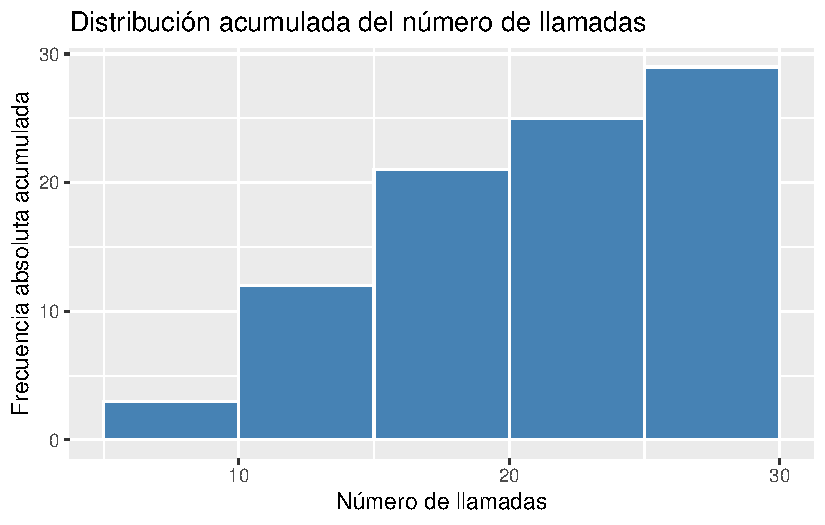
\includegraphics[keepaspectratio]{04-frecuencias-graficos_files/figure-pdf/unnamed-chunk-18-3.pdf}}

\begin{Shaded}
\begin{Highlighting}[]
\CommentTok{\# Histograma de frecuencias relativas acumuladas}
\CommentTok{\# Añadimos la variable a la dimensión x.}
\NormalTok{df }\SpecialCharTok{|\textgreater{}} \FunctionTok{ggplot}\NormalTok{(}\FunctionTok{aes}\NormalTok{(}\AttributeTok{x =}\NormalTok{ urgencias)) }\SpecialCharTok{+}
    \CommentTok{\# Añadimos la geometría de histograma y asignamos a la dimensión y las frecuencias relativas acumuladas. }
    \FunctionTok{geom\_histogram}\NormalTok{(}\FunctionTok{aes}\NormalTok{(}\AttributeTok{y =} \FunctionTok{after\_stat}\NormalTok{(}\FunctionTok{cumsum}\NormalTok{(count)}\SpecialCharTok{/}\FunctionTok{sum}\NormalTok{(count))),  }\AttributeTok{breaks =} \FunctionTok{seq}\NormalTok{(}\DecValTok{5}\NormalTok{, }\DecValTok{30}\NormalTok{, }\DecValTok{5}\NormalTok{), }\AttributeTok{fill =} \StringTok{"steelblue"}\NormalTok{, }\AttributeTok{col =} \StringTok{"white"}\NormalTok{) }\SpecialCharTok{+}

    \FunctionTok{labs}\NormalTok{(}\AttributeTok{title =} \StringTok{"Distribución acumulada del número de urgencias"}\NormalTok{, }\AttributeTok{x =} \StringTok{"Número de urgencias"}\NormalTok{, }\AttributeTok{y =} \StringTok{"Frecuencia relativa acumulada"}\NormalTok{)}
\end{Highlighting}
\end{Shaded}

  \pandocbounded{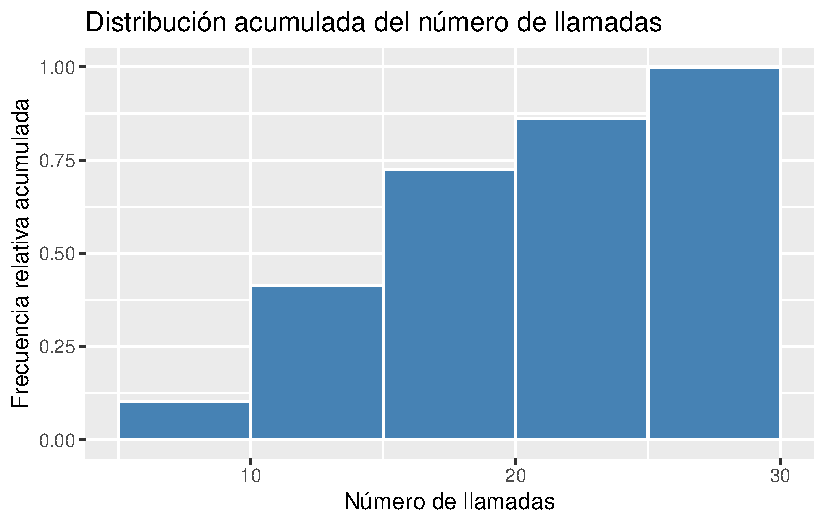
\includegraphics[keepaspectratio]{04-frecuencias-graficos_files/figure-pdf/unnamed-chunk-18-4.pdf}}

  \end{tcolorbox}
\item
  Dibujar el polígono de frecuencias relativas acumuladas (ojiva).

  \begin{tcolorbox}[enhanced jigsaw, breakable, leftrule=.75mm, toptitle=1mm, rightrule=.15mm, opacitybacktitle=0.6, left=2mm, colframe=quarto-callout-tip-color-frame, titlerule=0mm, toprule=.15mm, opacityback=0, bottomtitle=1mm, coltitle=black, colbacktitle=quarto-callout-tip-color!10!white, title=\textcolor{quarto-callout-tip-color}{\faLightbulb}\hspace{0.5em}{Solución}, arc=.35mm, bottomrule=.15mm, colback=white]

  \section{Base}

  Para dibujar el polígono de frecuencias relativas acumuladas podemos
  usar la función
  \href{https://www.rdocumentation.org/packages/graphics/versions/3.6.2/topics/plot}{\texttt{plot}}
  del paquete \texttt{graphics}.

  Parámetros:

  \begin{itemize}
  \tightlist
  \item
    \texttt{x}: vector con las coordenadas x de los vértices del
    polígono.
  \item
    \texttt{y}: vector con las coordenadas y de los vértices del
    polígono.
  \item
    \texttt{type}: tipo de gráfico. Para un polígono de frecuencias se
    usa \texttt{"l"} (línea).
  \item
    \texttt{col}: color de la línea.
  \item
    \texttt{main}: título del gráfico.
  \item
    \texttt{xlab}: etiqueta del eje x.
  \item
    \texttt{ylab}: etiqueta del eje y.
  \end{itemize}

\begin{Shaded}
\begin{Highlighting}[]
\CommentTok{\# Ojiva}
\CommentTok{\# Definimos los puntos de corte de los intervalos.}
\NormalTok{cortes }\OtherTok{=} \FunctionTok{seq}\NormalTok{(}\DecValTok{5}\NormalTok{, }\DecValTok{30}\NormalTok{, }\DecValTok{5}\NormalTok{)}
\CommentTok{\# Calculamos las frecuencias absolutas agrupando en 5 clases.}
\NormalTok{ni }\OtherTok{\textless{}{-}} \FunctionTok{table}\NormalTok{(}\FunctionTok{cut}\NormalTok{(df}\SpecialCharTok{$}\NormalTok{urgencias, }\AttributeTok{breaks =}\NormalTok{ cortes))}
\CommentTok{\# Calculamos las frecuencias relativas acumuladas.}
\NormalTok{Fi }\OtherTok{\textless{}{-}} \FunctionTok{c}\NormalTok{(}\DecValTok{0}\NormalTok{, }\FunctionTok{cumsum}\NormalTok{(ni)}\SpecialCharTok{/}\FunctionTok{sum}\NormalTok{(ni))}
\CommentTok{\# Dibujamos el polígono de frecuencias relativas acumuladas.}
\FunctionTok{plot}\NormalTok{(cortes, Fi, }\AttributeTok{type =} \StringTok{"l"}\NormalTok{, }\AttributeTok{col =} \StringTok{"steelblue"}\NormalTok{, }\AttributeTok{main =} \StringTok{"Distribución acumulada del número de urgencias"}\NormalTok{, }\AttributeTok{xlab =} \StringTok{"Número de urgencias"}\NormalTok{, }\AttributeTok{ylab =} \StringTok{"Frecuencia relativa acumulada"}\NormalTok{)}
\end{Highlighting}
\end{Shaded}

  \pandocbounded{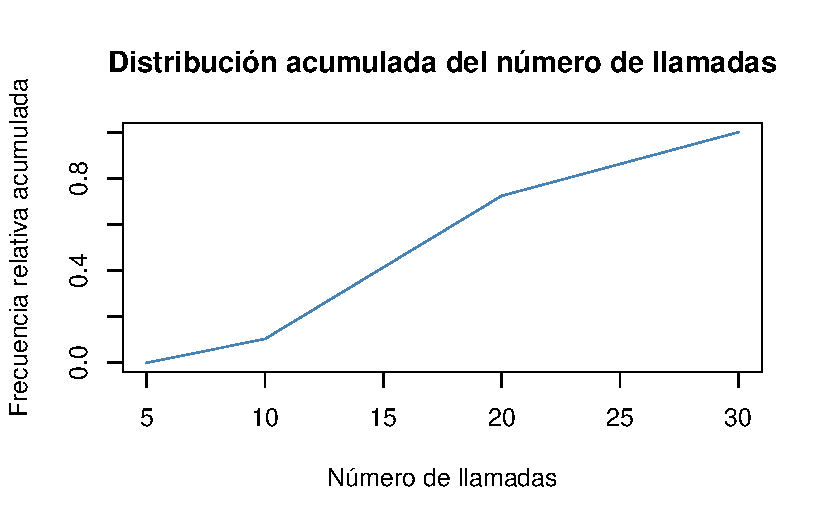
\includegraphics[keepaspectratio]{04-frecuencias-graficos_files/figure-pdf/unnamed-chunk-19-1.pdf}}

  \section{tidyverse}

  Para dibujar el polígono de frecuencias relativas acumuladas podemos
  usar la función
  \href{https://aprendeconalf.es/manual-r/07-graficos.html\#histogramas}{\texttt{geom\_line}}
  del paquete \texttt{ggplot2} de \texttt{tidyverse}.

\begin{Shaded}
\begin{Highlighting}[]
\CommentTok{\# Ojiva}
\CommentTok{\# Definimos los puntos de corte de los intervalos.}
\NormalTok{cortes }\OtherTok{\textless{}{-}} \FunctionTok{seq}\NormalTok{(}\DecValTok{5}\NormalTok{, }\DecValTok{30}\NormalTok{, }\DecValTok{5}\NormalTok{)}
\CommentTok{\# Añadimos una nueva columna al data frame con la clase a la que pertenece cada individuo, tomando 5 intervalos desde 5 hasta 30.}
\NormalTok{tabla\_frec }\OtherTok{\textless{}{-}}\NormalTok{ df }\SpecialCharTok{|\textgreater{}} \FunctionTok{mutate}\NormalTok{(}\AttributeTok{urgencias\_int =} \FunctionTok{cut}\NormalTok{(df}\SpecialCharTok{$}\NormalTok{urgencias, }\AttributeTok{breaks =}\NormalTok{ cortes)) }\SpecialCharTok{|\textgreater{}} 
    \CommentTok{\# Calculamos las frecuencias absolutas de cada clase.}
    \FunctionTok{count}\NormalTok{(urgencias\_int) }\SpecialCharTok{|\textgreater{}}
    \CommentTok{\# Añadimos una nueva columna con las frecuencias relativas acumuladas.}
    \FunctionTok{mutate}\NormalTok{(}\AttributeTok{cortes =}\NormalTok{ cortes[}\SpecialCharTok{{-}}\DecValTok{1}\NormalTok{], }\AttributeTok{Fi =} \FunctionTok{cumsum}\NormalTok{(n)}\SpecialCharTok{/}\FunctionTok{sum}\NormalTok{(n)) }\SpecialCharTok{|\textgreater{}}
    \CommentTok{\# Seleccionamos las columnas que nos interesan.}
    \FunctionTok{select}\NormalTok{(cortes, Fi) }
\CommentTok{\# Añadimos una fila con el primer punto de corte y frecuencia relativa acumulada 0.}
\NormalTok{tabla\_frec }\OtherTok{\textless{}{-}} \FunctionTok{rbind}\NormalTok{(}\FunctionTok{data.frame}\NormalTok{(}\AttributeTok{cortes =}\NormalTok{ cortes[}\DecValTok{1}\NormalTok{], }\AttributeTok{Fi =} \DecValTok{0}\NormalTok{), tabla\_frec)}
\CommentTok{\# Dibujamos el polígono de frecuencias relativas acumuladas.}
\CommentTok{\# Añadimos los cortes a la dimensión x y las frecuencias relativas acumuladas a}
\FunctionTok{ggplot}\NormalTok{(tabla\_frec, }\FunctionTok{aes}\NormalTok{(}\AttributeTok{x =}\NormalTok{ cortes , }\AttributeTok{y =}\NormalTok{ Fi)) }\SpecialCharTok{+}
    \CommentTok{\# Añadimos la geometría de líneas.}
    \FunctionTok{geom\_line}\NormalTok{(}\AttributeTok{col =} \StringTok{"steelblue"}\NormalTok{) }\SpecialCharTok{+}
    \CommentTok{\# Añadimos el título y las etiquetas de los ejes.}
    \FunctionTok{labs}\NormalTok{(}\AttributeTok{title =} \StringTok{"Distribución del número de urgencias"}\NormalTok{, }\AttributeTok{x =} \StringTok{"Número de urgencias"}\NormalTok{, }\AttributeTok{y =} \StringTok{"Frecuencia relativa acumulada"}\NormalTok{)}
\end{Highlighting}
\end{Shaded}

  \pandocbounded{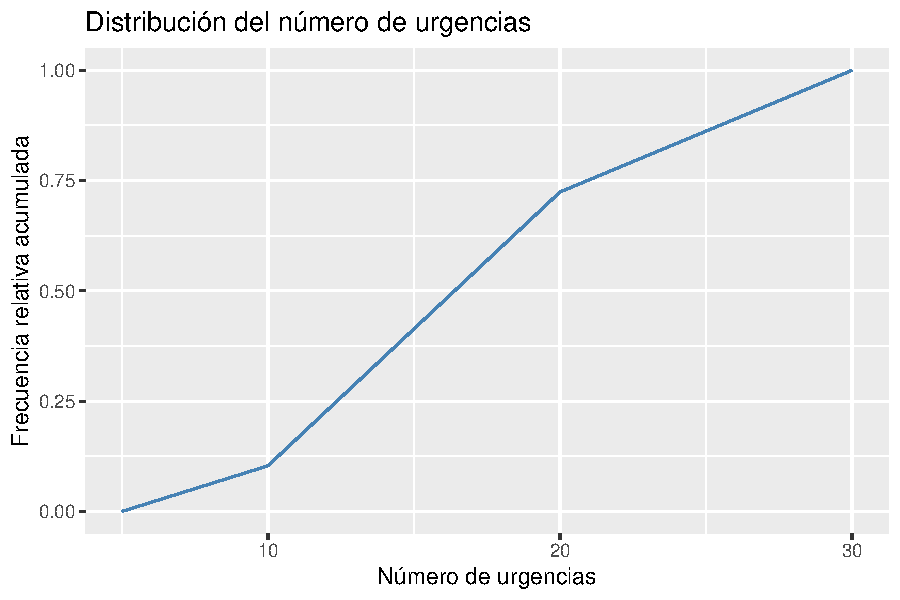
\includegraphics[keepaspectratio]{04-frecuencias-graficos_files/figure-pdf/unnamed-chunk-20-1.pdf}}

  \end{tcolorbox}
\end{enumerate}

\end{exercise}

\begin{exercise}[]\protect\hypertarget{exr-frecuencias-graficos-grupo-sanguineo}{}\label{exr-frecuencias-graficos-grupo-sanguineo}

Los grupos sanguíneos de una muestra de 30 personas son:

\[
\begin{array}{c}
\mbox{A, B, B, A, AB, 0, 0, A, B, B, A, A, A, A, AB, A, A, A, B, 0, B, B, B, A, A, A, 0, A, AB, 0}
\end{array}
\]

\begin{enumerate}
\def\labelenumi{\alph{enumi}.}
\item
  Crear un conjunto de datos con la variable \texttt{grupo\_sanguíneo}.

  \begin{tcolorbox}[enhanced jigsaw, breakable, leftrule=.75mm, toptitle=1mm, rightrule=.15mm, opacitybacktitle=0.6, left=2mm, colframe=quarto-callout-tip-color-frame, titlerule=0mm, toprule=.15mm, opacityback=0, bottomtitle=1mm, coltitle=black, colbacktitle=quarto-callout-tip-color!10!white, title=\textcolor{quarto-callout-tip-color}{\faLightbulb}\hspace{0.5em}{Solución}, arc=.35mm, bottomrule=.15mm, colback=white]

  \section{Base}

\begin{Shaded}
\begin{Highlighting}[]
\NormalTok{df }\OtherTok{\textless{}{-}} \FunctionTok{data.frame}\NormalTok{(}\AttributeTok{grupo\_sanguineo =} \FunctionTok{c}\NormalTok{(}\StringTok{"A"}\NormalTok{, }\StringTok{"B"}\NormalTok{, }\StringTok{"B"}\NormalTok{, }\StringTok{"A"}\NormalTok{, }\StringTok{"AB"}\NormalTok{, }\StringTok{"0"}\NormalTok{, }\StringTok{"0"}\NormalTok{, }\StringTok{"A"}\NormalTok{, }\StringTok{"B"}\NormalTok{, }\StringTok{"B"}\NormalTok{, }\StringTok{"A"}\NormalTok{, }\StringTok{"A"}\NormalTok{, }\StringTok{"A"}\NormalTok{, }\StringTok{"A"}\NormalTok{, }\StringTok{"AB"}\NormalTok{, }\StringTok{"A"}\NormalTok{, }\StringTok{"A"}\NormalTok{, }\StringTok{"A"}\NormalTok{, }\StringTok{"B"}\NormalTok{, }\StringTok{"0"}\NormalTok{, }\StringTok{"B"}\NormalTok{, }\StringTok{"B"}\NormalTok{, }\StringTok{"B"}\NormalTok{, }\StringTok{"A"}\NormalTok{, }\StringTok{"A"}\NormalTok{, }\StringTok{"A"}\NormalTok{, }\StringTok{"0"}\NormalTok{, }\StringTok{"A"}\NormalTok{, }\StringTok{"AB"}\NormalTok{, }\StringTok{"0"}\NormalTok{))}
\end{Highlighting}
\end{Shaded}

  \section{tidyverse}

\begin{Shaded}
\begin{Highlighting}[]
\FunctionTok{library}\NormalTok{(tidyverse)}
\NormalTok{df }\OtherTok{\textless{}{-}} \FunctionTok{tibble}\NormalTok{(}\AttributeTok{grupo\_sanguineo =} \FunctionTok{c}\NormalTok{(}\StringTok{"A"}\NormalTok{, }\StringTok{"B"}\NormalTok{, }\StringTok{"B"}\NormalTok{, }\StringTok{"A"}\NormalTok{, }\StringTok{"AB"}\NormalTok{, }\StringTok{"0"}\NormalTok{, }\StringTok{"0"}\NormalTok{, }\StringTok{"A"}\NormalTok{, }\StringTok{"B"}\NormalTok{, }\StringTok{"B"}\NormalTok{, }\StringTok{"A"}\NormalTok{, }\StringTok{"A"}\NormalTok{, }\StringTok{"A"}\NormalTok{, }\StringTok{"A"}\NormalTok{, }\StringTok{"AB"}\NormalTok{, }\StringTok{"A"}\NormalTok{, }\StringTok{"A"}\NormalTok{, }\StringTok{"A"}\NormalTok{, }\StringTok{"B"}\NormalTok{, }\StringTok{"0"}\NormalTok{, }\StringTok{"B"}\NormalTok{, }\StringTok{"B"}\NormalTok{, }\StringTok{"B"}\NormalTok{, }\StringTok{"A"}\NormalTok{, }\StringTok{"A"}\NormalTok{, }\StringTok{"A"}\NormalTok{, }\StringTok{"0"}\NormalTok{, }\StringTok{"A"}\NormalTok{, }\StringTok{"AB"}\NormalTok{, }\StringTok{"0"}\NormalTok{))}
\end{Highlighting}
\end{Shaded}

  \end{tcolorbox}
\item
  Construir la tabla de frecuencias.

  \begin{tcolorbox}[enhanced jigsaw, breakable, leftrule=.75mm, toptitle=1mm, rightrule=.15mm, opacitybacktitle=0.6, left=2mm, colframe=quarto-callout-tip-color-frame, titlerule=0mm, toprule=.15mm, opacityback=0, bottomtitle=1mm, coltitle=black, colbacktitle=quarto-callout-tip-color!10!white, title=\textcolor{quarto-callout-tip-color}{\faLightbulb}\hspace{0.5em}{Solución}, arc=.35mm, bottomrule=.15mm, colback=white]

  \section{Base}

  Para obtener las frecuencias absolutas se puede usar la función
  \href{https://www.rdocumentation.org/packages/base/versions/3.6.2/topics/table}{\texttt{table}},
  y para las frecuencias relativas la función
  \href{https://www.rdocumentation.org/packages/base/versions/3.6.2/topics/prop.table}{\texttt{prop.table}}
  ambas del paquete base de R.

\begin{Shaded}
\begin{Highlighting}[]
\FunctionTok{library}\NormalTok{(knitr)}
\CommentTok{\# Frecuencias absolutas.}
\NormalTok{ni }\OtherTok{\textless{}{-}} \FunctionTok{table}\NormalTok{(df}\SpecialCharTok{$}\NormalTok{grupo\_sanguineo)}
\CommentTok{\# Frecuencias relativas}
\NormalTok{fi }\OtherTok{\textless{}{-}} \FunctionTok{prop.table}\NormalTok{(ni)}
\NormalTok{tabla\_frec }\OtherTok{\textless{}{-}} \FunctionTok{cbind}\NormalTok{(ni, fi)}
\FunctionTok{kable}\NormalTok{(tabla\_frec)}
\end{Highlighting}
\end{Shaded}

  \begin{longtable}[]{@{}lrr@{}}
  \toprule\noalign{}
  & ni & fi \\
  \midrule\noalign{}
  \endhead
  \bottomrule\noalign{}
  \endlastfoot
  0 & 5 & 0.1666667 \\
  A & 14 & 0.4666667 \\
  AB & 3 & 0.1000000 \\
  B & 8 & 0.2666667 \\
  \end{longtable}

  \section{tidyverse}

  Para obtener la tabla de frecuencias absolutas podemos usar la función
  \href{https://aprendeconalf.es/manual-r/06-preprocesamiento.html\#conteo-del-n\%C3\%BAmero-de-observaciones}{\texttt{count}}
  del paquete \texttt{dplyr} de \texttt{tidyverse}.

  Posteriormente podemos añadir nuevas columnas a la tabla de
  frecuencias mediante la función \texttt{mutate} y la fórmula para
  calcular las frecuencias relativas (\texttt{n/sum(n)}).

\begin{Shaded}
\begin{Highlighting}[]
\FunctionTok{library}\NormalTok{(knitr)}
\CommentTok{\# Calculamos la tabla de frecuencias absolutas.}
\NormalTok{df }\SpecialCharTok{|\textgreater{}} \FunctionTok{count}\NormalTok{(grupo\_sanguineo) }\SpecialCharTok{|\textgreater{}} 
    \CommentTok{\# Añadimos una nueva columna con las frecuencias relativas.}
    \FunctionTok{mutate}\NormalTok{(}\AttributeTok{fi =}\NormalTok{ n}\SpecialCharTok{/}\FunctionTok{sum}\NormalTok{(n)) }\SpecialCharTok{|\textgreater{}}
    \FunctionTok{kable}\NormalTok{()}
\end{Highlighting}
\end{Shaded}

  \begin{longtable}[]{@{}lrr@{}}
  \toprule\noalign{}
  grupo\_sanguineo & n & fi \\
  \midrule\noalign{}
  \endhead
  \bottomrule\noalign{}
  \endlastfoot
  0 & 5 & 0.1666667 \\
  A & 14 & 0.4666667 \\
  AB & 3 & 0.1000000 \\
  B & 8 & 0.2666667 \\
  \end{longtable}

  \end{tcolorbox}
\item
  Dibujar el diagrama de sectores.

  \begin{tcolorbox}[enhanced jigsaw, breakable, leftrule=.75mm, toptitle=1mm, rightrule=.15mm, opacitybacktitle=0.6, left=2mm, colframe=quarto-callout-tip-color-frame, titlerule=0mm, toprule=.15mm, opacityback=0, bottomtitle=1mm, coltitle=black, colbacktitle=quarto-callout-tip-color!10!white, title=\textcolor{quarto-callout-tip-color}{\faLightbulb}\hspace{0.5em}{Solución}, arc=.35mm, bottomrule=.15mm, colback=white]

  \section{Base}

  Para dibujar el diagrama de sectores podemos usar la función
  \href{https://www.rdocumentation.org/packages/graphics/versions/3.6.2/topics/pie}{\texttt{pie}}
  del paquete \texttt{graphics}.

  Parámetros:

  \begin{itemize}
  \tightlist
  \item
    \texttt{x}: vector con las frecuencias.
  \item
    \texttt{col}: vector con los colores de los sectores.
  \item
    \texttt{main}: título del gráfico.
  \end{itemize}

\begin{Shaded}
\begin{Highlighting}[]
\FunctionTok{pie}\NormalTok{(ni, }\AttributeTok{col =} \DecValTok{1}\SpecialCharTok{:}\FunctionTok{length}\NormalTok{(ni), }\AttributeTok{main =} \StringTok{"Distribución de los grupos sanguíneos"}\NormalTok{)}
\end{Highlighting}
\end{Shaded}

  \pandocbounded{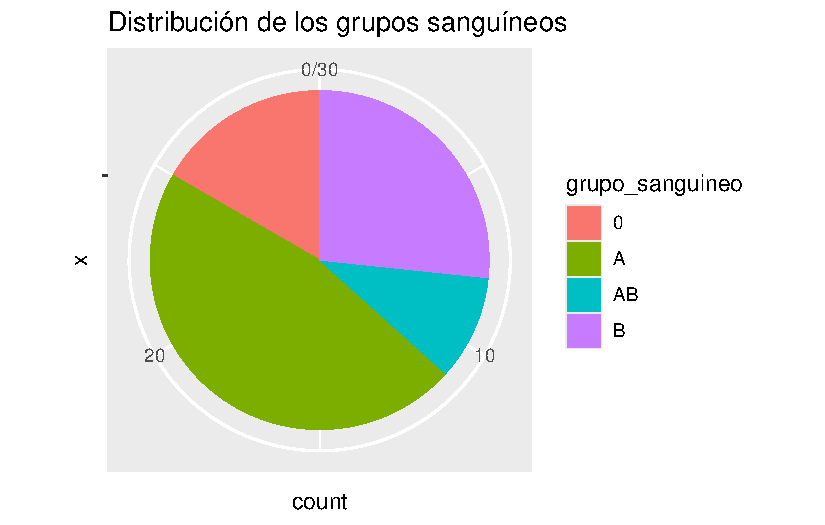
\includegraphics[keepaspectratio]{04-frecuencias-graficos_files/figure-pdf/unnamed-chunk-25-1.pdf}}

  \section{tidyverse}

  Para dibujar el diagrama de sectores podemos usar la función
  \href{https://aprendeconalf.es/manual-r/07-graficos.html\#diagrama-de-sectores}{\texttt{geom\_bar}}
  y después la función \texttt{coor\_polar} del paquete \texttt{ggplot2}
  de \texttt{tidyverse}.

  Parámetros:

  \begin{itemize}
  \tightlist
  \item
    \texttt{theta} = Dimensión que contiene las frecuencias.
  \end{itemize}

\begin{Shaded}
\begin{Highlighting}[]
\CommentTok{\# Añadimos la variable a la dimensión fill, y dejamos la dimensión x vacía.}
\NormalTok{df }\SpecialCharTok{|\textgreater{}} \FunctionTok{ggplot}\NormalTok{(}\FunctionTok{aes}\NormalTok{(}\AttributeTok{x =} \StringTok{""}\NormalTok{, }\AttributeTok{fill =}\NormalTok{ grupo\_sanguineo)) }\SpecialCharTok{+}
    \CommentTok{\# Añadimos la geometría de barras.}
    \FunctionTok{geom\_bar}\NormalTok{(}\AttributeTok{color =} \StringTok{"white"}\NormalTok{) }\SpecialCharTok{+}
    \CommentTok{\# Cambiamos a coordenadas polares.}
    \FunctionTok{coord\_polar}\NormalTok{(}\AttributeTok{theta =} \StringTok{"y"}\NormalTok{) }\SpecialCharTok{+}
    \CommentTok{\# Añadimos el título y las etiquetas de los ejes.}
    \FunctionTok{labs}\NormalTok{(}\AttributeTok{title =} \StringTok{"Distribución de los grupos sanguíneos"}\NormalTok{, }\AttributeTok{fill =} \StringTok{"Grupo sanguíneo"}\NormalTok{) }\SpecialCharTok{+}
    \CommentTok{\# Eliminamos los ejes y el fondo del gráfico.}
    \FunctionTok{theme\_void}\NormalTok{() }
\end{Highlighting}
\end{Shaded}

  \pandocbounded{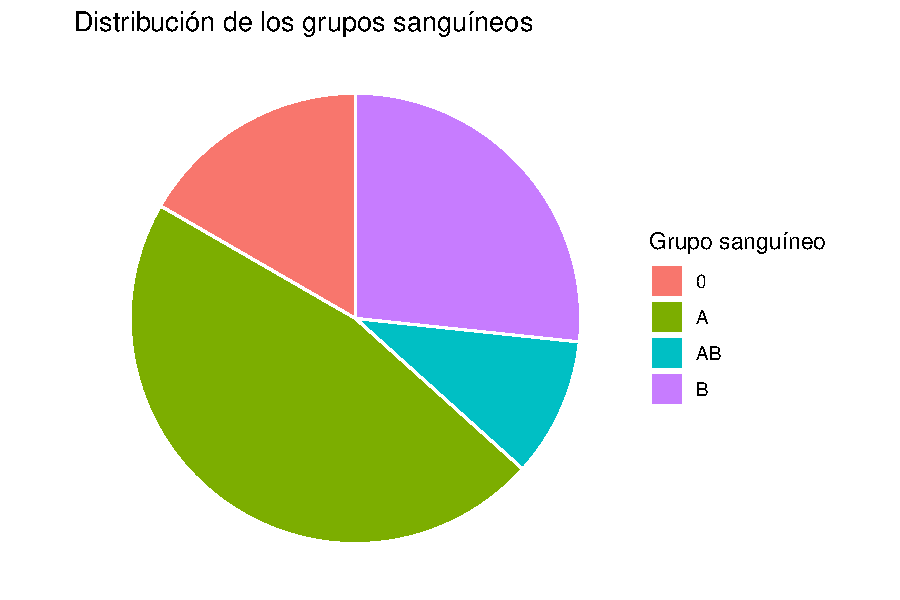
\includegraphics[keepaspectratio]{04-frecuencias-graficos_files/figure-pdf/unnamed-chunk-26-1.pdf}}

  \end{tcolorbox}
\end{enumerate}

\end{exercise}

\begin{exercise}[]\protect\hypertarget{exr-frecuencias-graficos-estado-civil-edades}{}\label{exr-frecuencias-graficos-estado-civil-edades}

En un estudio de población se tomó una muestra de 27 personas, y se les
preguntó por su edad y estado civil, obteniendo los siguientes
resultados:

\begin{longtable}[]{@{}ll@{}}
\toprule\noalign{}
Estado civil & Edad \\
\midrule\noalign{}
\endhead
\bottomrule\noalign{}
\endlastfoot
Soltero & 31, 45, 35, 65, 21, 38, 62, 22, 31 \\
Casado & 62, 39, 62, 59, 21, 62 \\
Viudo & 80, 68, 65, 40, 78, 69, 75 \\
Divorciado & 31, 65, 59, 49, 65 \\
\end{longtable}

\begin{enumerate}
\def\labelenumi{\alph{enumi}.}
\item
  Crear un conjunto de datos con la variables \texttt{estado\_civil} y
  \texttt{edad}.

  \begin{tcolorbox}[enhanced jigsaw, breakable, leftrule=.75mm, toptitle=1mm, rightrule=.15mm, opacitybacktitle=0.6, left=2mm, colframe=quarto-callout-tip-color-frame, titlerule=0mm, toprule=.15mm, opacityback=0, bottomtitle=1mm, coltitle=black, colbacktitle=quarto-callout-tip-color!10!white, title=\textcolor{quarto-callout-tip-color}{\faLightbulb}\hspace{0.5em}{Solución}, arc=.35mm, bottomrule=.15mm, colback=white]

  \section{Base}

\begin{Shaded}
\begin{Highlighting}[]
\NormalTok{df }\OtherTok{\textless{}{-}} \FunctionTok{data.frame}\NormalTok{(}
    \AttributeTok{edad =} \FunctionTok{c}\NormalTok{(}\DecValTok{31}\NormalTok{, }\DecValTok{45}\NormalTok{, }\DecValTok{35}\NormalTok{, }\DecValTok{65}\NormalTok{, }\DecValTok{21}\NormalTok{, }\DecValTok{38}\NormalTok{, }\DecValTok{62}\NormalTok{, }\DecValTok{22}\NormalTok{, }\DecValTok{31}\NormalTok{, }\DecValTok{62}\NormalTok{, }\DecValTok{39}\NormalTok{, }\DecValTok{62}\NormalTok{, }\DecValTok{59}\NormalTok{, }\DecValTok{21}\NormalTok{, }\DecValTok{62}\NormalTok{, }\DecValTok{80}\NormalTok{, }\DecValTok{68}\NormalTok{, }\DecValTok{65}\NormalTok{, }\DecValTok{40}\NormalTok{, }\DecValTok{78}\NormalTok{, }\DecValTok{69}\NormalTok{, }\DecValTok{75}\NormalTok{, }\DecValTok{31}\NormalTok{, }\DecValTok{65}\NormalTok{, }\DecValTok{59}\NormalTok{, }\DecValTok{49}\NormalTok{, }\DecValTok{65}\NormalTok{), }
    \AttributeTok{estado\_civil =} \FunctionTok{rep}\NormalTok{(}\FunctionTok{c}\NormalTok{(}\StringTok{"Soltero"}\NormalTok{, }\StringTok{"Casado"}\NormalTok{, }\StringTok{"Viudo"}\NormalTok{, }\StringTok{"Divorciado"}\NormalTok{), }\FunctionTok{c}\NormalTok{(}\DecValTok{9}\NormalTok{, }\DecValTok{6}\NormalTok{, }\DecValTok{7}\NormalTok{, }\DecValTok{5}\NormalTok{)))}
\end{Highlighting}
\end{Shaded}

  \section{tidyverse}

\begin{Shaded}
\begin{Highlighting}[]
\NormalTok{df }\OtherTok{\textless{}{-}} \FunctionTok{tibble}\NormalTok{(}
    \AttributeTok{edad =} \FunctionTok{c}\NormalTok{(}\DecValTok{31}\NormalTok{, }\DecValTok{45}\NormalTok{, }\DecValTok{35}\NormalTok{, }\DecValTok{65}\NormalTok{, }\DecValTok{21}\NormalTok{, }\DecValTok{38}\NormalTok{, }\DecValTok{62}\NormalTok{, }\DecValTok{22}\NormalTok{, }\DecValTok{31}\NormalTok{, }\DecValTok{62}\NormalTok{, }\DecValTok{39}\NormalTok{, }\DecValTok{62}\NormalTok{, }\DecValTok{59}\NormalTok{, }\DecValTok{21}\NormalTok{, }\DecValTok{62}\NormalTok{, }\DecValTok{80}\NormalTok{, }\DecValTok{68}\NormalTok{, }\DecValTok{65}\NormalTok{, }\DecValTok{40}\NormalTok{, }\DecValTok{78}\NormalTok{, }\DecValTok{69}\NormalTok{, }\DecValTok{75}\NormalTok{, }\DecValTok{31}\NormalTok{, }\DecValTok{65}\NormalTok{, }\DecValTok{59}\NormalTok{, }\DecValTok{49}\NormalTok{, }\DecValTok{65}\NormalTok{), }
    \AttributeTok{estado\_civil =} \FunctionTok{rep}\NormalTok{(}\FunctionTok{c}\NormalTok{(}\StringTok{"Soltero"}\NormalTok{, }\StringTok{"Casado"}\NormalTok{, }\StringTok{"Viudo"}\NormalTok{, }\StringTok{"Divorciado"}\NormalTok{), }\FunctionTok{c}\NormalTok{(}\DecValTok{9}\NormalTok{, }\DecValTok{6}\NormalTok{, }\DecValTok{7}\NormalTok{, }\DecValTok{5}\NormalTok{)))}
\end{Highlighting}
\end{Shaded}

  \end{tcolorbox}
\item
  Calcular las frecuencias absolutas del \texttt{estado\_civil}.

  \begin{tcolorbox}[enhanced jigsaw, breakable, leftrule=.75mm, toptitle=1mm, rightrule=.15mm, opacitybacktitle=0.6, left=2mm, colframe=quarto-callout-tip-color-frame, titlerule=0mm, toprule=.15mm, opacityback=0, bottomtitle=1mm, coltitle=black, colbacktitle=quarto-callout-tip-color!10!white, title=\textcolor{quarto-callout-tip-color}{\faLightbulb}\hspace{0.5em}{Solución}, arc=.35mm, bottomrule=.15mm, colback=white]

  \section{Base}

  Para obtener las frecuencias absolutas se puede usar la función
  \href{https://www.rdocumentation.org/packages/base/versions/3.6.2/topics/table}{\texttt{table}}
  del paquete base de R.

\begin{Shaded}
\begin{Highlighting}[]
\FunctionTok{library}\NormalTok{(knitr)}
\FunctionTok{table}\NormalTok{(df}\SpecialCharTok{$}\NormalTok{estado\_civil) }\SpecialCharTok{|\textgreater{}} \FunctionTok{kable}\NormalTok{()}
\end{Highlighting}
\end{Shaded}

  \begin{longtable}[]{@{}lr@{}}
  \toprule\noalign{}
  Var1 & Freq \\
  \midrule\noalign{}
  \endhead
  \bottomrule\noalign{}
  \endlastfoot
  Casado & 6 \\
  Divorciado & 5 \\
  Soltero & 9 \\
  Viudo & 7 \\
  \end{longtable}

  \section{tidyverse}

  Para obtener la tabla de frecuencias absolutas podemos usar la función
  \href{https://aprendeconalf.es/manual-r/06-preprocesamiento.html\#conteo-del-n\%C3\%BAmero-de-observaciones}{\texttt{count}}
  del paquete \texttt{dplyr} de \texttt{tidyverse}.

\begin{Shaded}
\begin{Highlighting}[]
\FunctionTok{library}\NormalTok{(knitr)}
\CommentTok{\# Calculamos las frecuencias absolutas del estado civil.}
\NormalTok{df }\SpecialCharTok{|\textgreater{}} \FunctionTok{count}\NormalTok{(estado\_civil)}
\end{Highlighting}
\end{Shaded}

  \begin{longtable}[]{@{}lr@{}}
  \toprule\noalign{}
  estado\_civil & n \\
  \midrule\noalign{}
  \endhead
  \bottomrule\noalign{}
  \endlastfoot
  Casado & 6 \\
  Divorciado & 5 \\
  Soltero & 9 \\
  Viudo & 7 \\
  \end{longtable}

  \end{tcolorbox}
\item
  Construir la tabla de frecuencias de la variable \texttt{edad} para
  cada categoría de la variable \texttt{estado\_civil}.

  \begin{tcolorbox}[enhanced jigsaw, breakable, leftrule=.75mm, toptitle=1mm, rightrule=.15mm, opacitybacktitle=0.6, left=2mm, colframe=quarto-callout-tip-color-frame, titlerule=0mm, toprule=.15mm, opacityback=0, bottomtitle=1mm, coltitle=black, colbacktitle=quarto-callout-tip-color!10!white, title=\textcolor{quarto-callout-tip-color}{\faLightbulb}\hspace{0.5em}{Solución}, arc=.35mm, bottomrule=.15mm, colback=white]

  Para dividir el data frame en grupos podemos usar la función
  \href{https://aprendeconalf.es/manual-r/06-preprocesamiento.html\#res\%C3\%BAmenes-por-grupos}{\texttt{group-by}}
  del paquete \texttt{dplyr} de \texttt{tidyverse} indicando la variable
  de agrupación.

  Después podemos usar la función
  \href{https://aprendeconalf.es/manual-r/06-preprocesamiento.html\#conteo-del-n\%C3\%BAmero-de-observaciones}{\texttt{count}}
  del paquete \texttt{dplyr} de \texttt{tidyverse} para obtener la tabla
  de frecuencias absolutas.

\begin{Shaded}
\begin{Highlighting}[]
\CommentTok{\# Añadimos una nueva columna al data frame con la clase a la que pertenece cada individuo, tomando intervalos de amplitud 10 desde 20 hasta 80.}
\NormalTok{df }\SpecialCharTok{|\textgreater{}} \FunctionTok{mutate}\NormalTok{(}\AttributeTok{edad\_int =} \FunctionTok{cut}\NormalTok{(edad, }\AttributeTok{breaks =} \FunctionTok{seq}\NormalTok{(}\DecValTok{20}\NormalTok{, }\DecValTok{80}\NormalTok{, }\DecValTok{10}\NormalTok{))) }\SpecialCharTok{|\textgreater{}}
    \CommentTok{\# Agrupamos por estado civil.}
    \FunctionTok{group\_by}\NormalTok{(estado\_civil) }\SpecialCharTok{|\textgreater{}}
    \CommentTok{\# Calculamos las frecuencias absolutas.}
    \FunctionTok{count}\NormalTok{(edad\_int) }\SpecialCharTok{|\textgreater{}} 
    \CommentTok{\# Añadimos nuevas columnas con las frecuencias relativas, acumuladas y relativas acumuladas.}
    \FunctionTok{mutate}\NormalTok{(}\AttributeTok{fi =}\NormalTok{ n}\SpecialCharTok{/}\FunctionTok{sum}\NormalTok{(n), }\AttributeTok{Ni =} \FunctionTok{cumsum}\NormalTok{(n), }\AttributeTok{Fi =} \FunctionTok{cumsum}\NormalTok{(n)}\SpecialCharTok{/}\FunctionTok{sum}\NormalTok{(n)) }\SpecialCharTok{|\textgreater{}}
    \FunctionTok{kable}\NormalTok{()}
\end{Highlighting}
\end{Shaded}

  \begin{longtable}[]{@{}llrrrr@{}}
  \toprule\noalign{}
  estado\_civil & edad\_int & n & fi & Ni & Fi \\
  \midrule\noalign{}
  \endhead
  \bottomrule\noalign{}
  \endlastfoot
  Casado & (20,30{]} & 1 & 0.1666667 & 1 & 0.1666667 \\
  Casado & (30,40{]} & 1 & 0.1666667 & 2 & 0.3333333 \\
  Casado & (50,60{]} & 1 & 0.1666667 & 3 & 0.5000000 \\
  Casado & (60,70{]} & 3 & 0.5000000 & 6 & 1.0000000 \\
  Divorciado & (30,40{]} & 1 & 0.2000000 & 1 & 0.2000000 \\
  Divorciado & (40,50{]} & 1 & 0.2000000 & 2 & 0.4000000 \\
  Divorciado & (50,60{]} & 1 & 0.2000000 & 3 & 0.6000000 \\
  Divorciado & (60,70{]} & 2 & 0.4000000 & 5 & 1.0000000 \\
  Soltero & (20,30{]} & 2 & 0.2222222 & 2 & 0.2222222 \\
  Soltero & (30,40{]} & 4 & 0.4444444 & 6 & 0.6666667 \\
  Soltero & (40,50{]} & 1 & 0.1111111 & 7 & 0.7777778 \\
  Soltero & (60,70{]} & 2 & 0.2222222 & 9 & 1.0000000 \\
  Viudo & (30,40{]} & 1 & 0.1428571 & 1 & 0.1428571 \\
  Viudo & (60,70{]} & 3 & 0.4285714 & 4 & 0.5714286 \\
  Viudo & (70,80{]} & 3 & 0.4285714 & 7 & 1.0000000 \\
  \end{longtable}

  \end{tcolorbox}
\item
  Dibujar los diagramas de cajas de la edad según el estado civil.
  ¿Existen datos atípicos? ¿En qué grupo hay mayor dispersión?

  \begin{tcolorbox}[enhanced jigsaw, breakable, leftrule=.75mm, toptitle=1mm, rightrule=.15mm, opacitybacktitle=0.6, left=2mm, colframe=quarto-callout-tip-color-frame, titlerule=0mm, toprule=.15mm, opacityback=0, bottomtitle=1mm, coltitle=black, colbacktitle=quarto-callout-tip-color!10!white, title=\textcolor{quarto-callout-tip-color}{\faLightbulb}\hspace{0.5em}{Solución}, arc=.35mm, bottomrule=.15mm, colback=white]

  \section{Base}

  Para dibujar un diagrama de caja y bigotes podemos usar la función
  \href{https://www.rdocumentation.org/packages/graphics/versions/3.6.2/topics/boxplot}{\texttt{boxplot}}
  del paquete \texttt{graphics}.

  Parámetros:

  \begin{itemize}
  \tightlist
  \item
    \texttt{formula}: fórmula que relaciona la variable dependiente con
    la variable independiente (en este caso
    \texttt{edad\ \textasciitilde{}\ estado\_civil}).
  \item
    \texttt{data}: data frame con los datos.
  \item
    \texttt{col}: color de la caja.
  \item
    \texttt{horizontal}: orientación horizontal de la caja (True o
    False).
  \item
    \texttt{width}: anchura de la caja (valor entre 0 y 1).
  \item
    \texttt{main}: título del gráfico.
  \item
    \texttt{xlab}: etiqueta del eje x.
  \item
    \texttt{ylab}: etiqueta del eje y.
  \end{itemize}

\begin{Shaded}
\begin{Highlighting}[]
\FunctionTok{boxplot}\NormalTok{(edad }\SpecialCharTok{\textasciitilde{}}\NormalTok{ estado\_civil, }\AttributeTok{data =}\NormalTok{ df, }\AttributeTok{horizontal =}\NormalTok{ T, }\AttributeTok{col =} \StringTok{"steelblue"}\NormalTok{, }\AttributeTok{main =} \StringTok{"Distribución de la edad según el estado civil"}\NormalTok{, }\AttributeTok{xlab =} \StringTok{"Edad"}\NormalTok{, }\AttributeTok{ylab =} \StringTok{"Estado civil"}\NormalTok{)}
\end{Highlighting}
\end{Shaded}

  \pandocbounded{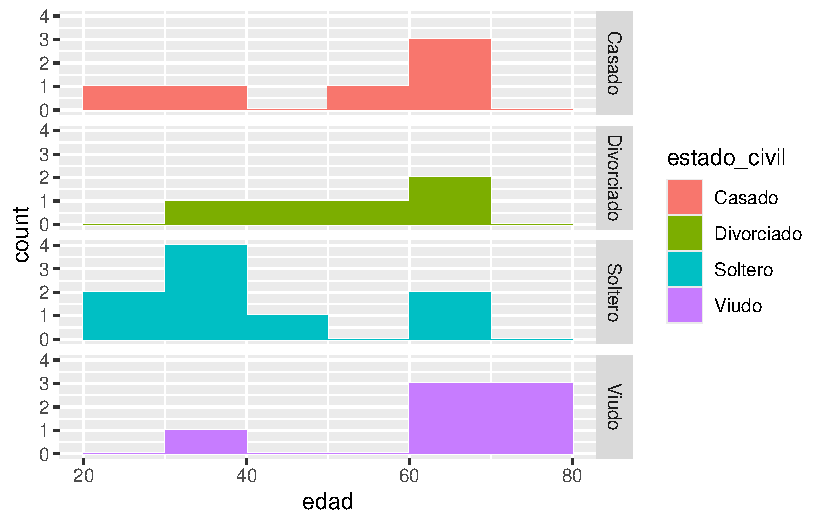
\includegraphics[keepaspectratio]{04-frecuencias-graficos_files/figure-pdf/unnamed-chunk-32-1.pdf}}

  \section{tidyverse}

  Para dibujar un diagrama de caja y bigotes podemos usar la función
  \href{https://aprendeconalf.es/manual-r/07-graficos.html\#diagramas-de-cajas}{\texttt{geom\_boxplot}}
  del paquete \texttt{ggplot2} de \texttt{tidyverse}.

  Parámetros:

  \begin{itemize}
  \tightlist
  \item
    color: color del borde de la caja.
  \item
    fill: factor con las categorías que dividen en grupos las cajas (en
    este caso \texttt{estado\_civil}). Dibuja una caja por cada
    categoría.
  \item
    width: anchura de la caja (valor entre 0 y 1).
  \end{itemize}

\begin{Shaded}
\begin{Highlighting}[]
\CommentTok{\# Añadimos la variable a la dimensión x y el estado civil a la dimensión fill.}
\NormalTok{df }\SpecialCharTok{|\textgreater{}} \FunctionTok{ggplot}\NormalTok{(}\FunctionTok{aes}\NormalTok{(}\AttributeTok{x =}\NormalTok{ edad, }\AttributeTok{fill =}\NormalTok{ estado\_civil)) }\SpecialCharTok{+}
    \CommentTok{\# Añadimos la geometría de cajas.}
    \FunctionTok{geom\_boxplot}\NormalTok{() }\SpecialCharTok{+}
    \CommentTok{\# Eliminamos las marcas del eje y.}
    \FunctionTok{scale\_y\_continuous}\NormalTok{(}\AttributeTok{breaks =} \ConstantTok{NULL}\NormalTok{) }\SpecialCharTok{+}
    \CommentTok{\# Añadimos el título y las etiquetas de los ejes y leyenda.}
    \FunctionTok{labs}\NormalTok{(}\AttributeTok{title =} \StringTok{"Distribución de la edad según el estado civil"}\NormalTok{, }\AttributeTok{x =} \StringTok{"Edad"}\NormalTok{, }\AttributeTok{fill =} \StringTok{"Estado civil"}\NormalTok{) }
\end{Highlighting}
\end{Shaded}

  \pandocbounded{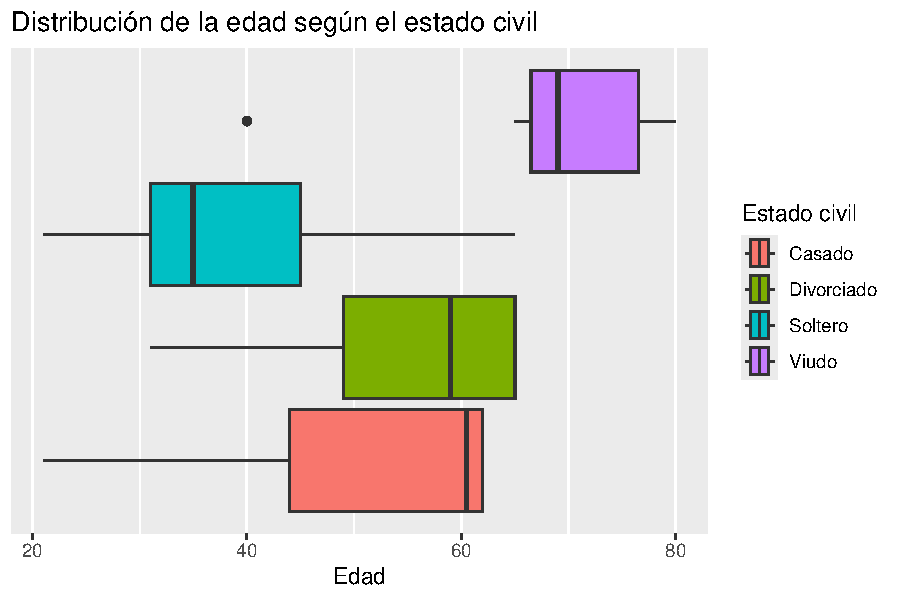
\includegraphics[keepaspectratio]{04-frecuencias-graficos_files/figure-pdf/unnamed-chunk-33-1.pdf}}

  \end{tcolorbox}
\item
  Dibujar los histogramas de la edad según el estado civil.

  \begin{tcolorbox}[enhanced jigsaw, breakable, leftrule=.75mm, toptitle=1mm, rightrule=.15mm, opacitybacktitle=0.6, left=2mm, colframe=quarto-callout-tip-color-frame, titlerule=0mm, toprule=.15mm, opacityback=0, bottomtitle=1mm, coltitle=black, colbacktitle=quarto-callout-tip-color!10!white, title=\textcolor{quarto-callout-tip-color}{\faLightbulb}\hspace{0.5em}{Solución}, arc=.35mm, bottomrule=.15mm, colback=white]

  Para dibujar un histograma podemos usar la
  función\href{https://aprendeconalf.es/manual-r/07-graficos.html\#histogramas}{\texttt{geom\_histogram}}
  del paquete \texttt{ggplot2} de \texttt{tidyverse}.

  Parámetros:

  \begin{itemize}
  \tightlist
  \item
    \texttt{breaks}: Un vector con los puntos de corte de los intervalos
    de las barras.
  \item
    \texttt{color}: Color del borde de las barras.
  \item
    \texttt{fill}: factor con las categorías que dividen en grupos las
    cajas (en este caso \texttt{estado\_civil}). Dibuja una caja por
    cada categoría.
  \item
    \texttt{position}: Posición de las barras (``identity'' para
    superponer las barras, ``stack'' para apilar las barras y ``dodge''
    para que las barras no se superpongan).
  \item
    \texttt{alpha}: Transparencia de las barras (valor entre 0 y 1).
  \end{itemize}

\begin{Shaded}
\begin{Highlighting}[]
\CommentTok{\# Añadimos la variable a la dimensión x y el estado civil a la dimensión fill.}
\NormalTok{df }\SpecialCharTok{|\textgreater{}} \FunctionTok{ggplot}\NormalTok{(}\FunctionTok{aes}\NormalTok{(}\AttributeTok{x =}\NormalTok{ edad, }\AttributeTok{fill =}\NormalTok{ estado\_civil)) }\SpecialCharTok{+}
    \CommentTok{\# Añadimos la geometría de histograma creando clases de amplitud 10 desde 20 hasta 80.}
    \FunctionTok{geom\_histogram}\NormalTok{(}\AttributeTok{breaks =} \FunctionTok{seq}\NormalTok{(}\DecValTok{20}\NormalTok{, }\DecValTok{80}\NormalTok{, }\DecValTok{10}\NormalTok{), }\AttributeTok{position =} \StringTok{"stack"}\NormalTok{) }\SpecialCharTok{+}
    \CommentTok{\# Añadimos el título y las etiquetas de los ejes.}
    \FunctionTok{labs}\NormalTok{(}\AttributeTok{title =} \StringTok{"Distribución de la edad según el estado civil"}\NormalTok{, }\AttributeTok{x =} \StringTok{"Edad"}\NormalTok{, }\AttributeTok{y =} \StringTok{"Frecuencia"}\NormalTok{, }\AttributeTok{fill =} \StringTok{"Estado civil"}\NormalTok{) }
\end{Highlighting}
\end{Shaded}

  \pandocbounded{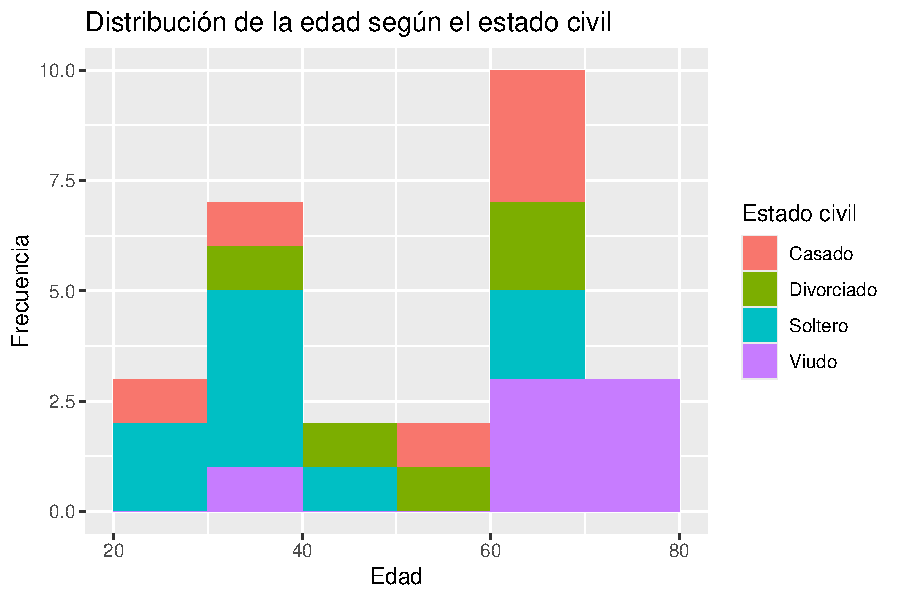
\includegraphics[keepaspectratio]{04-frecuencias-graficos_files/figure-pdf/unnamed-chunk-34-1.pdf}}

  Para dibujar cada histograma por separado se puede usar la función
  \href{https://aprendeconalf.es/manual-r/07-graficos.html\#facetas}{\texttt{facet\_wrap}}
  o \texttt{facet\_grid} del paquete \texttt{ggplot2} de
  \texttt{tidyverse}.

\begin{Shaded}
\begin{Highlighting}[]
\CommentTok{\# Añadimos la variable a la dimensión x y el estado civil a la dimensión fill.}
\NormalTok{df }\SpecialCharTok{|\textgreater{}} \FunctionTok{ggplot}\NormalTok{(}\FunctionTok{aes}\NormalTok{(}\AttributeTok{x =}\NormalTok{ edad, }\AttributeTok{fill =}\NormalTok{ estado\_civil)) }\SpecialCharTok{+}
   \CommentTok{\# Añadimos la geometría de histograma creando clases de amplitud 10 desde 20 hasta 80.}
    \FunctionTok{geom\_histogram}\NormalTok{(}\AttributeTok{breaks =} \FunctionTok{seq}\NormalTok{(}\DecValTok{20}\NormalTok{, }\DecValTok{80}\NormalTok{, }\DecValTok{10}\NormalTok{)) }\SpecialCharTok{+}
    \CommentTok{\# Añadimos facetas el estado civil.}
    \FunctionTok{facet\_wrap}\NormalTok{(}\SpecialCharTok{\textasciitilde{}}\NormalTok{ estado\_civil) }\SpecialCharTok{+}
    \CommentTok{\# Añadimos el título y las etiquetas de los ejes.}
    \FunctionTok{labs}\NormalTok{(}\AttributeTok{title =} \StringTok{"Distribución de la edad según el estado civil"}\NormalTok{, }\AttributeTok{x =} \StringTok{"Edad"}\NormalTok{, }\AttributeTok{y =} \StringTok{"Frecuencia"}\NormalTok{, }\AttributeTok{fill =} \StringTok{"Estado civil"}\NormalTok{) }
\end{Highlighting}
\end{Shaded}

  \pandocbounded{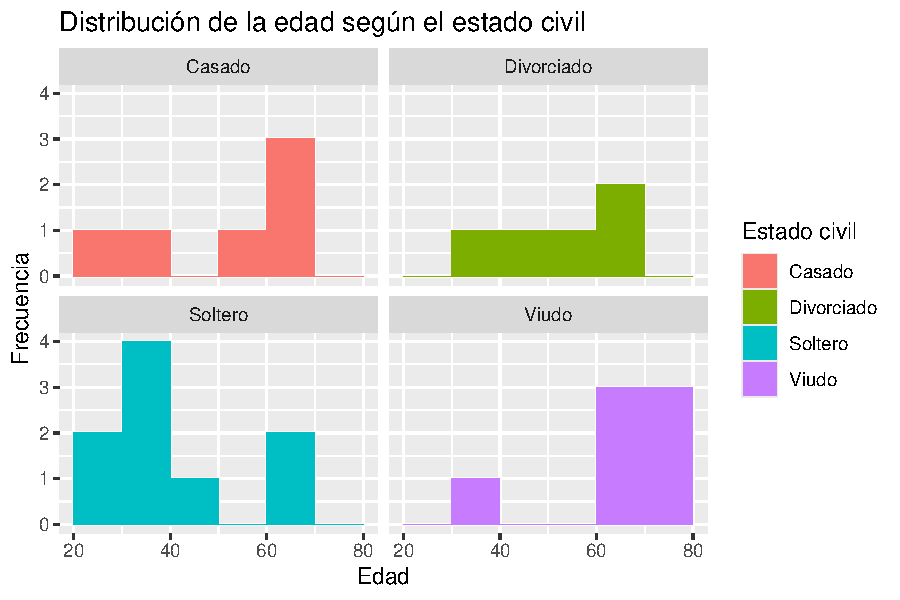
\includegraphics[keepaspectratio]{04-frecuencias-graficos_files/figure-pdf/unnamed-chunk-35-1.pdf}}

  \end{tcolorbox}
\end{enumerate}

\end{exercise}

\section{Ejercicios propuestos}\label{ejercicios-propuestos-2}

\begin{exercise}[]\protect\hypertarget{exr-frecuencias-graficos-neonatos}{}\label{exr-frecuencias-graficos-neonatos}

El conjunto de datos \href{datos/neonatos.csv}{neonatos} contiene
información sobre una muestra de 320 recién nacidos en un hospital
durante un año que cumplieron el tiempo normal de gestación.

\begin{enumerate}
\def\labelenumi{\alph{enumi}.}
\item
  Construir la tabla de frecuencias de la puntuación Apgar al minuto de
  nacer. Si se considera que una puntuación Apgar de 3 o menos indica
  que el neonato está deprimido, ¿qué porcentaje de niños está deprimido
  en la muestra?
\item
  Comparar las distribuciones de frecuencias de las puntuaciones Apgar
  al minuto de nacer según si la madre es mayor o menor de 20 años. ¿En
  qué grupo hay más neonatos deprimidos?
\item
  Construir la tabla de frecuencias para el peso de los neonatos,
  agrupando en clases de amplitud \(0.5\) desde el \(2\) hasta el
  \(4.5\). ¿En qué intervalo de peso hay más neonatos?
\item
  Comparar la distribución de frecuencias relativas del peso de los
  neonatos según si la madre fuma o no. Si se considera como peso bajo
  un peso menor de \(2.5\) kg, ¿En qué grupo hay un mayor porcentaje de
  niños con peso bajo?
\item
  Construir el diagrama de barras de la puntuación Apgar al minuto. ¿Qué
  puntuación Apgar es la más frecuente?
\item
  Construir el diagrama de frecuencias relativas acumuladas de la
  puntuación Apgar al minuto. ¿Por debajo de que puntuación estarán la
  mitad de los niños?
\item
  Comparar mediante diagramas de barras de frecuencias relativas las
  distribuciones de las puntuaciones Apgar al minuto según si la madre
  ha fumado o no durante el embarazo. ¿Qué se puede concluir?
\item
  Construir el histograma de pesos, agrupando en clases de amplitud
  \(0.5\) desde el \(2\) hasta el \(4.5\). ¿En qué intervalo de peso hay
  más niños?
\item
  Comparar la distribución de frecuencias relativas del peso de los
  neonatos según si la madre fuma o no. ¿En qué grupo se aprecia menor
  peso de los niños de la muestra?
\item
  Comparar la distribución de frecuencias relativas del peso de los
  neonatos según si la madre fumaba o no antes del embarazo. ¿Qué se
  puede concluir?
\item
  Construir el diagrama de caja y bigotes del peso. ¿Entre qué valores
  se considera que el peso de un neonato es normal? ¿Existen datos
  atípicos?
\item
  Comparar el diagrama de cajas y bigotes del peso, según si la madre
  fumó o no durante el embarazo y si era mayor o no de 20 años. ¿En qué
  grupo el peso tiene más dispersión central? ¿En qué grupo pesan menos
  los niños de la muestra?
\item
  Comparar el diagrama de cajas de la puntuación Apgar al minuto y a los
  cinco minutos. ¿En qué variable hay más dispersión central?
\end{enumerate}

\end{exercise}




\end{document}
